% ========== Template by IC\M/T Institute of Creative\Media/Technologies =============
% ==========  M. Wagner and K. Blumenstein, N. Thuer 2017 ============= 
% ==========  Based on the LaTeX Thesis Template for the University of Applied Sciences St.Pölten by P. Lechner https://github.com/hrtlacek/ThesisTemplate-FH-StP        ============= 

%----------------------------------------------------------------
% TODO List


%----------------------------------------------------------------

%Dokumentklasse without end dot ;-)
\documentclass[a4paper,twoside,11pt, numbers=noenddot]{scrreprt}
\usepackage[left= 3.5cm,right = 3cm, bottom = 3.5 cm, top = 3 cm]{geometry}
\usepackage[onehalfspacing]{setspace}

% Standard Packages
\usepackage[utf8]{inputenc}

% ============= Settings for the Work =============

\def\workTitle{Isolierte und automatisierte Vernetzung von
Internetdiensten in einer hybriden
Cloud-Infrastruktur}
\def\subTitle{~}
\def\specialization{<Name of Masterclass>}
\def\studentFirstName{Justus}
\def\studentLastName{Mungard}
\def\studentId{931 221}
\def\advisorPreTitle{Dipl.-Inform.}
\def\advisoFirstName{Corina}
\def\advisorLastName{Kopka}
\def\advisorCompanyPreTitle{Dr.}
\def\advisorCompanyFirstName{Roland}
\def\advisorCompanyLastName{Kaltefleiter}
\def\advisorPosTitle{}
\def\assessorPreTitle{}
\def\assessorFirstName{}
\def\assessorLastName{}
\def\assessorPosTitle{}
\def\place{Kiel}
\def\dateDay{20}
\def\dateMonth{05}
\def\dateYear{2021}

\newif\ifuseGermanVersion				    % <== DONT TOUCH THIS!!!
\newif\ifuseMasterInteractiveTechnologies 	% <== CAN'T TOUCH THIS!!! (da da dada)
\newif\ifuseMasterDigitalDesign	            % <== DONT TOUCH THIS!!!
\newif\ifuseMasterDigitalMediaProduction	% <== DONT TOUCH THIS!!!
\newif\ifuseMasterDigitalHealthCare			% <== DONT TOUCH THIS!!!
\newif\ifuseBachelorMediaTechnologiesOne    % <== DONT TOUCH THIS!!!
\newif\ifuseBachelorMediaTechnologiesTwo    % <== DONT TOUCH THIS!!!
\newif\ifuseBachelorSmartEngineeringOne     % <== DONT TOUCH THIS!!!
\newif\ifuseBachelorSmartEngineeringTwo     % <== DONT TOUCH THIS!!!

%***************************************************************************************
% To switch the version please use the comment "%" option :-). After a language change, you have to rebuild the whole project (in Overleaf --> recompile from scratch) 
\useGermanVersiontrue					    % German version
%\useGermanVersionfalse					    % English version
%***************************************************************************************
% To switch between the study programs use the comment option :-) 
% !!!ATTENTION: Only one has to be activated!!!
\useBachelorMediaTechnologiesOnetrue		% Bachelor #1 Media Technology
%\useBachelorMediaTechnologiesTwotrue		% Bachelor #2 Media Technology
%\useMasterInteractiveTechnologiestrue		% Master Interactive Technologies
%\useMasterDigitalDesigntrue		        % Master Digital Design
%\useMasterDigitalMediaProductiontrue		% Master Digital Media Production
%\useMasterDigitalHealthCaretrue			% Master Digital Health Care
% \useBachelorSmartEngineeringOnetrue		% Bachelor #1 Smart Engineering
%\useBachelorSmartEngineeringTwotrue		% Bachelor #2 Smart Engineering
%***************************************************************************************
% Dokumentinformationen
\usepackage[
	pdftitle={\workTitle},
	pdfsubject={},
	pdfauthor={\studentFirstName \studentLastName},
	pdfkeywords={}
	pdftex=true, 
	colorlinks=true,
 	breaklinks=true,
	citecolor=black,
	linkcolor=black,	
	menucolor=black,	
	%urlcolor=black
	urlcolor=magenta
]{hyperref}

\hypersetup{
    bookmarks=true,         % show bookmarks bar?
    unicode=false,          % non-Latin characters in Acrobat’s bookmarks
    pdftoolbar=true,        % show Acrobat’s toolbar?
    pdfmenubar=true,        % show Acrobat’s menu?
    pdffitwindow=false,     % window fit to page when opened
    pdfstartview={FitH},    % fits the width of the page to the window
    pdftitle={My title},    % title
    pdfauthor={Author},     % author
    pdfsubject={Subject},   % subject of the document
    pdfcreator={Creator},   % creator of the document
    pdfproducer={Producer}, % producer of the document
    pdfkeywords={keyword1} {key2} {key3}, % list of keywords
    pdfnewwindow=true,      % links in new window
    colorlinks=false,       % false: boxed links; true: colored links
    linkcolor=black,          % color of internal links (change box color with linkbordercolor)
    citecolor=black,        % color of links to bibliography
    filecolor=black,      % color of file links
    urlcolor=black           % color of external links
}

\usepackage{xurl}
\usepackage{chngcntr}
\usepackage{placeins}
\usepackage{enumitem}
\usepackage[disabled]{todonotes}
\usepackage[toc,acronym]{glossaries}
%https://tex.stackexchange.com/questions/116534/lstlisting-line-wrapping/116572
%https://tex.stackexchange.com/questions/269491/mixing-minted-with-lstlisting
\usepackage[chapter]{minted}
\AtEndEnvironment{listing}{\vspace{-14pt}}

% ============= Packages =============

% Dokumentinformationen
\usepackage[
	pdftitle={\workTitle},
	pdfsubject={},
	pdfauthor={\studentFirstName \studentLastName},
	pdfkeywords={}
	pdftex=true, 
	colorlinks=true,
 	breaklinks=true,
	citecolor=black,
	linkcolor=black,	
	menucolor=black,	
	%urlcolor=black
	urlcolor=magenta
]{hyperref}

\hypersetup{
    bookmarks=true,         % show bookmarks bar?
    unicode=false,          % non-Latin characters in Acrobat’s bookmarks
    pdftoolbar=true,        % show Acrobat’s toolbar?
    pdfmenubar=true,        % show Acrobat’s menu?
    pdffitwindow=false,     % window fit to page when opened
    pdfstartview={FitH},    % fits the width of the page to the window
    pdftitle={My title},    % title
    pdfauthor={Author},     % author
    pdfsubject={Subject},   % subject of the document
    pdfcreator={Creator},   % creator of the document
    pdfproducer={Producer}, % producer of the document
    pdfkeywords={keyword1} {key2} {key3}, % list of keywords
    pdfnewwindow=true,      % links in new window
    colorlinks=false,       % false: boxed links; true: colored links
    linkcolor=black,          % color of internal links (change box color with linkbordercolor)
    citecolor=black,        % color of links to bibliography
    filecolor=black,      % color of file links
    urlcolor=black           % color of external links
}

% Switch the Language
\ifuseGermanVersion
	\usepackage[ngerman]{babel}	% German
\else
	\usepackage[english]{babel} % English
\fi
\usepackage{csquotes}

\usepackage[T1]{fontenc}
%\usepackage{graphicx}
\usepackage{graphicx, subfigure}
%Set path for images
%\graphicspath{{img/}}
\usepackage{fancyhdr}
\usepackage{lmodern}
\usepackage{color}
\usepackage{transparent}

% Zitierstil
% Citation style
%\usepackage[comma,authoryear]{natbib}
%\usepackage{natbib}

%\usepackage[backend=biber, style=apa, citestyle=authoryear, sorting=nyt]{biblatex}

%\ifuseGermanVersion
%    \DeclareLanguageMapping{ngerman}{ngerman-apa}
%\else
%    \DeclareLanguageMapping{english}{english-apa}
%\fi

\usepackage[nottoc]{tocbibind}
%\addbibresource{biblatex.bib}

% zusätzliche Schriftzeichen der American Mathematical Society
\usepackage{amsfonts}
\usepackage{mathtools}

\usepackage[export]{adjustbox}

% BlockDiagram Drawing Package
% ---tikz
\usepackage{tikz}
\usetikzlibrary{positioning}
\usepackage{pgfplots}
\pgfplotsset{compat=1.10}
\usepackage{textcomp}

%====================================================
% Code Block Style Definition
%\documentclass{article}
\usepackage[utf8]{inputenc}

\usepackage{listings}
\usepackage{xcolor}

\definecolor{codegreen}{rgb}{0,0.6,0}
\definecolor{codegray}{rgb}{0.5,0.5,0.5}
\definecolor{codepurple}{rgb}{0.58,0,0.82}
\definecolor{backcolour}{rgb}{0.95,0.95,0.92}

\lstdefinestyle{mystyle}{
    backgroundcolor=\color{backcolour},   
    commentstyle=\color{codegreen},
    keywordstyle=\color{magenta},
    numberstyle=\tiny\color{codegray},
    stringstyle=\color{codepurple},
    basicstyle=\ttfamily\footnotesize,
    breakatwhitespace=false,         
    breaklines=true,                 
    captionpos=b,                    
    keepspaces=true,                 
    numbers=left,                    
    numbersep=5pt,                  
    showspaces=false,                
    showstringspaces=false,
    showtabs=false,                  
    tabsize=2
}

\lstset{style=mystyle}

%Try minted
%https://tex.stackexchange.com/questions/116534/lstlisting-line-wrapping/116572
\usepackage{lmodern} % for bold teletype font
\usepackage{minted}

%====================================================

%Package for using the [H] option on graphics to force them into place
\usepackage{float}

%iPython packages:
%\usepackage{graphicx} % Used to insert images
\usepackage{adjustbox} % Used to constrain images to a maximum size 
\usepackage{color} % Allow colors to be defined
%\usepackage{enumerate} % Needed for markdown enumerations to work
\usepackage{geometry} % Used to adjust the document margins
\usepackage{amsmath} % Equations
\usepackage{amssymb} % Equations
%\usepackage[mathletters]{ucs} % Extended unicode (utf-8) support
% \usepackage[utf8x]{inputenc} % Allow utf-8 characters in the tex document
\usepackage{fancyvrb} % verbatim replacement that allows latex
\usepackage{grffile} % extends the file name processing of package graphics 
                         % to support a larger range 
    % The hyperref package gives us a pdf with properly built
    % internal navigation ('pdf bookmarks' for the table of contents,
    % internal cross-reference links, web links for URLs, etc.)
\usepackage{hyperref}
\usepackage{longtable} % longtable support required by pandoc >1.10

% embedding of audio/video files etc.
% \usepackage{attachfile}
% \usepackage{movie15}
% \usepackage{media9}
% \usepackage{menukeys}

\usepackage[labelfont=it, labelsep=period, format=plain,justification=raggedright, singlelinecheck=false]{caption}
\captionsetup[figure]{justification=centering}
\definecolor{light-gray}{gray}{0.85}

% Switch between German and English based on the Settingx.tex. file
\usepackage{ifthen}

%\captionsetup[listing]{
%  labelsep = newline,
%  textfont = sc, 
%  name = LISTING, 
%  justification=justified,
%  singlelinecheck=false,%%%%%%% a single line is centered by default
%  labelsep=colon,%%%%%%
%  skip = \medskipamount}

% =============== BlockDiagram Drawing Config
\usetikzlibrary{shapes,arrows}

% Definition of blocks:
\tikzset{%
  block/.style    = {draw, thick, rectangle, minimum height = 3em,
    minimum width = 3em},
  sum/.style      = {draw, circle, node distance = 2cm}, % Adder
  input/.style    = {coordinate}, % Input
  output/.style   = {coordinate}, % Output
  mult/.style	  = {draw, isosceles triangle, minimum height=1cm, minimum width =1cm}
}
%mult/.style	  = {isosceles triangle, sharp corners, anchor=center, xshift=-4mm, minimum height=1.5cm, minimum width =0.05cm}
%isosceles triangle, fill=gray!25, minimum width=1.5cm

% Defining string as labels of certain blocks.
\newcommand{\suma}{\Large$+$}
\newcommand{\inte}{$\displaystyle \int$}
\newcommand{\derv}{\huge$\frac{d}{dt}$}
\newcommand{\conv}{\huge$\ast$}

% ============================================

% -- Settings für Code abbildungen
\usepackage{listings,lstautogobble}
\lstset{backgroundcolor=\color{light-gray},frame=single, framerule=0pt, showspaces=false, showtabs=false, numbers=left, numbersep=5pt, breaklines=false, autogobble=true, language=C++}

% Setze arial font
\usepackage[scaled]{helvet}
\renewcommand*{\familydefault}{\sfdefault}

% FH-grünBlau
\definecolor{FH}{rgb}{0.10, 0.57, 0.68}
% FH-grünBlau 2
\definecolor{FH2}{rgb}{0.0392, 0.666, 0.549}

% nicht einrücken nach Absatz
\setlength{\parindent}{0cm}

% Paragraph-Abstand
\setlength{\parskip}{0.3cm}

% ============= Kopf- und Fußzeile =============

%\renewcommand{\headrulewidth}{0.4pt}
%\renewcommand{\footrulewidth}{0pt}

\renewcommand{\chaptermark}[1]{\markboth{\thechapter~ #1}{}}

\fancypagestyle{icmt-fancy}{%
  \fancyhf{}% Clear header and footer
  \fancyhead[L]{\leftmark}
  \fancyfoot[R]{\thepage}% Custom footer
  \renewcommand{\headrulewidth}{0.4pt}% Line at the header visible
  \renewcommand{\footrulewidth}{0.0pt}% Line at the footer visible
}

% Redefine the plain page style
\fancypagestyle{plain}{%
  \fancyhf{}%
  \fancyfoot[R]{\thepage}%
  \renewcommand{\headrulewidth}{0pt}% Line at the header invisible
  \renewcommand{\footrulewidth}{0.0pt}% Line at the footer visible
}

% ============= Package Einstellungen & Sonstiges ============= 


%Besondere Trennungen
\hyphenation{De-zi-mal-tren-nung St-rei-fen-licht-scan-nern}

%römische Aufzählungen mit \RM{Zahl}
\newcommand{\RM}[1]{\MakeUppercase{\romannumeral #1}}


% ============= Dokumentbeginn =============

\begin{document}

% Select the right main page ;-)
\ifuseGermanVersion
	
% setup page dimensions for titlepage
\newgeometry{left=2.4cm,right=2.4cm,bottom=2.5cm,top=2cm}

% force baselineskip and parindent
%\newlength{\tmpbaselineskip}
%\setlength{\tmpbaselineskip}{\baselineskip}
%\setlength{\baselineskip}{13.6pt}
%\newlength{\tmpparindent}
%\setlength{\tmpparindent}{\parindent}
%\setlength{\parindent}{17pt}

% first titlepage
\pagestyle{empty}

\begin{figure}[H]
\vspace*{-2.5cm}
\hspace*{2.5cm}

\includegraphics[keepaspectratio, width=1.31\textwidth, right]{TemplateElements/Fachhochschule_Kiel-logo.svg.png}
\end{figure}



\begin{center}

\vspace{1cm}

\begin{minipage}[t][5cm][s]{\textwidth}%
\centering
\Huge{{\color{FH2}{\fontsize{24}{30} \selectfont \workTitle\\}}}
\vspace{0.5cm}
\LARGE{{\color{FH2}{\fontsize{16}{24} \selectfont \subTitle\\}}}
\end{minipage}

\vspace{1cm}


\ifnum\ifuseBachelorMediaTechnologiesOne 1
\else\ifuseBachelorSmartEngineeringOne 1
\else0
\fi\fi
=1 
   	\LARGE{Bachelorarbeit}
\else
	\ifnum\ifuseBachelorMediaTechnologiesTwo 2
	\else\ifuseBachelorSmartEngineeringTwo 2
\else0
\fi\fi
=2
	\LARGE{Bachelorarbeit}
\else
	\ifuseMasterInteractiveTechnologies
		\LARGE{Masterarbeit}
	\else
	\ifuseMasterDigitalDesign
		\LARGE{Masterarbeit}
	\else
    \ifuseMasterDigitalMediaProduction
		\LARGE{Masterarbeit}
	\else
	\ifuseMasterDigitalHealthCare
		\LARGE{Masterarbeit}
    \else
        \LARGE{YOU HAVE TO CHOOSE THE PROGRAM TYPE IN THE SETTINGS!!!}
    \fi\fi\fi\fi
\fi\fi

% \ifuseBachelorMediaTechnologiesOne
% 	\LARGE{Research Paper}
% \else
% 	\ifuseBachelorSmartEngineeringOne
%     	\LARGE{Research Paper}
% \else
% 	\ifuseBachelorMediaTechnologiesTwo
% 		\LARGE{Bachelorarbeit}
% \else
% 	\ifuseMasterDigitalMediaTechnologies
% 		\LARGE{Masterarbeit}
% \else
% 	\ifuseMasterDigitalHealthCare
% 		\LARGE{Masterarbeit}
%     \else
%         \LARGE{YOU HAVE TO CHOOSE THE PROGRAM TYPE IN THE SETTINGS!!!}
%   	\fi
% \fi
% \fi
% \fi
% \fi




\vspace{1.3cm}
\ifuseBachelorMediaTechnologiesOne
	\fontsize{11pt}{15pt}\selectfont Bachelor Informationstechnologie\\
	Fachbereich Informatik und Elektrotechnik\\
Fachhochschule Kiel University of Applied Sciences\\  
\else
	\ifuseBachelorMediaTechnologiesTwo
		\fontsize{11pt}{15pt}\selectfont Bachelor-Studiengang \\
Fachhochschule Kiel\\  
\else
	\ifuseBachelorSmartEngineeringOne
    	\fontsize{11pt}{15pt}\selectfont Bachelor-Studiengang Smart Engineering\\
Fachhochschule Kiel\\ 
\else
	\ifuseMasterInteractiveTechnologies
		\fontsize{11pt}{15pt}\selectfont Ausgeführt zum Zweck der Erlangung des akademischen Grades\\
		\textbf{Dipl.-Ing. für technisch-wissenschaftliche Berufe}
\else
	\ifuseMasterDigitalDesign
		\fontsize{11pt}{15pt}\selectfont Ausgeführt zum Zweck der Erlangung des akademischen Grades\\
		\textbf{Dipl.-Ing. für technisch-wissenschaftliche Berufe}	
\else
    \ifuseMasterDigitalMediaProduction
		\fontsize{11pt}{15pt}\selectfont Ausgeführt zum Zweck der Erlangung des akademischen Grades\\
		\textbf{Dipl.-Ing. für technisch-wissenschaftliche Berufe}	
\else
	\ifuseMasterDigitalHealthCare
    	\fontsize{11pt}{15pt}\selectfont Ausgeführt zum Zweck der Erlangung des akademischen Grades\\
		\textbf{Master of Science in Engineering (MSc)}
    \else
        \LARGE{YOU HAVE TO CHOOSE THE PROGRAM TYPE IN THE SETTINGS!!!}
\fi\fi\fi\fi\fi\fi\fi

\vspace{4mm}

\ifuseMasterInteractiveTechnologies
	am Masterstudiengang Interactive Technologies an der\\ 
Fachhochschule St. Pölten, Masterklasse \specialization
\else
    \ifuseMasterDigitalDesign
	am Masterstudiengang Digital Design an der\\ 
Fachhochschule St. Pölten, Masterklasse \specialization
\else
    \ifuseMasterDigitalMediaProduction
	am Masterstudiengang Digital Media Production an der\\ 
Fachhochschule St. Pölten, Masterklasse \specialization
\else
	\ifuseMasterDigitalHealthCare
		am Masterstudiengang Digital Healthcare\\ 
an der Fachhochschule St. Pölten
    \else
        
  	\fi\fi\fi\fi

\vspace{1cm}
\ifuseBachelorMediaTechnologiesOne
	Vorgelegt von:
    
\else
	Ausgeführt von:\\ 
\fi
\fontsize{15pt}{15pt}\selectfont
\textbf{\studentFirstName\ \studentLastName} \\
\fontsize{11pt}{15pt}\selectfont
\studentId

\vspace{1cm}
\ifuseBachelorMediaTechnologiesOne
	\begin{tabular}{lll}
    Erstprüferin: & & \advisorPreTitle\ \advisoFirstName\ 		\advisorLastName\\
    Zweitprüfer: & & \advisorCompanyPreTitle\ \advisorCompanyFirstName\ \advisorCompanyLastName\\
    \end{tabular}
\else
	\ifuseBachelorMediaTechnologiesTwo
		\begin{tabular}{lll}
        Betreuer/in: & & \advisorPreTitle\ \advisoFirstName\ \advisorLastName, \advisorPosTitle\\
        %Zweitbegutachter/in: & & [Titel Vorname Zuname]
		\end{tabular}
\else
\begin{tabular}{lll}
Betreuer/in: & \advisorPreTitle\ \advisoFirstName\ \advisorLastName, \advisorPosTitle\\
Zweitbetreuer/in: & \assessorPreTitle\ \assessorFirstName\ \assessorLastName, \assessorPosTitle\\
\end{tabular}

\fi
\fi

\vspace{1cm}


\large{\place, \dateDay.\dateMonth.\dateYear}


\end{center}

\restoregeometry
\else
	
% setup page dimensions for titlepage
\newgeometry{left=2.4cm,right=2.4cm,bottom=2.5cm,top=2cm}

% force baselineskip and parindent
%\newlength{\tmpbaselineskip}
%\setlength{\tmpbaselineskip}{\baselineskip}
%\setlength{\baselineskip}{13.6pt}
%\newlength{\tmpparindent}
%\setlength{\tmpparindent}{\parindent}
%\setlength{\parindent}{17pt}

% first titlepage
\pagestyle{empty}

\begin{figure}[H]
\vspace*{-2.5cm}
\hspace*{2.5cm}
\includegraphics[keepaspectratio, width=1.4\textwidth, right]{TemplateElements/fhLogo3.png}
\end{figure}



\begin{center}

\vspace{1cm}

\begin{minipage}[t][5cm][s]{\textwidth}%
\centering
\Huge{{\color{FH2}{\fontsize{24}{30} \selectfont \workTitle\\}}}
\vspace{0.5cm}
\LARGE{{\color{FH2}{\fontsize{16}{24} \selectfont \subTitle\\}}}
\end{minipage}

\vspace{1cm}

\ifuseBachelorMediaTechnologiesOne
	\LARGE{Research Paper}
\else
	\ifuseBachelorMediaTechnologiesTwo
		\LARGE{Bachelor Thesis}
\else
	\ifuseMasterInteractiveTechnologies
		\LARGE{Master Thesis}
\else
	\ifuseMasterDigitalDesign
		\LARGE{Master Thesis}
\else
    \ifuseMasterDigitalMediaProduction
		\LARGE{Master Thesis}
\else
	\ifuseMasterDigitalHealthCare
		\LARGE{Master Thesis}
    \else
        \LARGE{YOU HAVE TO CHOOSE THE PROGRAM TYPE IN THE SETTINGS!!!}
  	\fi
\fi
\fi
\fi\fi\fi
  
\vspace{1.3cm}
\ifuseBachelorMediaTechnologiesOne
	\fontsize{11pt}{15pt}\selectfont Bachelor Course on Media Technology\\
at St. Pölten University of Applied Sciences\\  
\else
	\ifuseBachelorMediaTechnologiesTwo
		\fontsize{11pt}{15pt}\selectfont Bachelor Course on Media Technology\\
at St. Pölten University of Applied Sciences\\  
\else
	\ifuseMasterInteractiveTechnologies
		\fontsize{11pt}{15pt}\selectfont For attainment of the academic degree of\\
		\textbf{Dipl.-Ing. für technisch-wissenschaftliche Berufe}
\else
    \ifuseMasterDigitalDesign
		\fontsize{11pt}{15pt}\selectfont For attainment of the academic degree of\\
		\textbf{Dipl.-Ing. für technisch-wissenschaftliche Berufe}
\else
    \ifuseMasterDigitalMediaProduction
		\fontsize{11pt}{15pt}\selectfont For attainment of the academic degree of\\
		\textbf{Dipl.-Ing. für technisch-wissenschaftliche Berufe}
\else
	\ifuseMasterDigitalHealthCare
    	\fontsize{11pt}{15pt}\selectfont For attainment of the academic degree of\\
		\textbf{Master of Science in Engineering (MSc)}
    \else
        \LARGE{YOU HAVE TO CHOOSE THE PROGRAM TYPE IN THE SETTINGS!!!}
  	\fi
\fi
\fi
\fi\fi\fi

\vspace{4mm}
 
\ifuseMasterInteractiveTechnologies
	in the Masters Course Interactive Technologies at St. Pölten\\ 
University of Applied Sciences, Masterclass \specialization
\else
    \ifuseMasterDigitalDesign
	in the Masters Course Digital Design at St. Pölten\\ 
University of Applied Sciences, Masterclass \specialization
\else
    \ifuseMasterDigitalMediaProduction
	in the Masters Course Digital Media Production at St. Pölten\\ 
University of Applied Sciences, Masterclass \specialization
\else
	\ifuseMasterDigitalHealthCare
		in the Masters Course Digital Healthcare\\ 
at St. Pölten University of Applied Sciences
    \else
  	\fi
\fi\fi\fi





\vspace{1cm}

Submitted by:\\ 
\fontsize{15pt}{15pt}\selectfont
\textbf{\studentFirstName\ \studentLastName} \\
\fontsize{11pt}{15pt}\selectfont
\studentId

\vspace{1cm}
\ifuseBachelorMediaTechnologiesOne
	\begin{tabular}{lll}
    Advisor: & & \advisorPreTitle\ \advisoFirstName\ 		\advisorLastName, \advisorPosTitle\\
    %Zweitbegutachter/in: & & [Titel Vorname Zuname]
    \end{tabular}
\else
	\ifuseBachelorMediaTechnologiesTwo
		\begin{tabular}{lll}
        Advisor: & & \advisorPreTitle\ \advisoFirstName\ \advisorLastName, \advisorPosTitle\\
        %Zweitbegutachter/in: & & [Titel Vorname Zuname]
		\end{tabular}
\else
  \begin{tabular}{lll}
  Advisor: & \advisorPreTitle\ \advisoFirstName\ \advisorLastName, \advisorPosTitle\\
  Second Advisor: & \assessorPreTitle\ \assessorFirstName\ \assessorLastName, \assessorPosTitle\\
  \end{tabular}

\fi
\fi

\vspace{1cm}


\large{\place, \dateDay.\dateMonth.\dateYear}


\end{center}

\restoregeometry
\fi

% \part im Inhaltsverzeichnis nicht nummerieren
\makeatletter
\let\partbackup\l@part
\renewcommand*\l@part[2]{\partbackup{#1}{}}

%Seitennummerierung neu beginnen, Zahlen [arabic], röm.Zahlen [roman,Roman], Buchstaben [alph,Alph]
\pagenumbering{Roman}

\newpage

\chapter*{Eidesstattliche Erklärung}
\label{ch:erklaerung}

\begin{flushleft}
Ich versichere mit meiner eigenhändigen Unterschrift, dass ich die vorliegende Abschlussarbeit selbständig und ohne unzulässige, fremde Hilfe angefertigt habe und dass ich alle von anderen Autor*innen wörtlich übernommenen Stellen wie auch die an die Gedankengänge und Strukturen anderer Autor*innen eng angelehnten Ausführungen meiner Arbeit besonders gekennzeichnet und die entsprechenden Quellen angegeben habe.
\end{flushleft}

\begin{flushleft}
Weiterhin versichere ich, dass die vorliegende Abschlussarbeit noch keiner Prüfungsbehörde vorgelegen hat.
\end{flushleft}

Ort: \hrulefill\enspace Datum:	\hrulefill\enspace Unterschrift: \hrulefill
\\[3.5cm]
\newpage

%Inhaltsverzeichnis
\pagestyle{plain}
\tableofcontents

\newpage
%Seitennummerierung neu beginnen, Zahlen [arabic], röm.Zahlen [roman,Roman], Buchstaben [alph,Alph]
\pagenumbering{arabic}

% pagestyle für gesamtes Dokument aktivieren
\pagestyle{icmt-fancy}
\newpage


\chapter{Einleitung}

Die NetUSE AG ist ein IT-Dienstleister aus Kiel mit den Schwerpunkten Infrastruktur, Security und Netzwerk. Viele Kunden der NetUSE AG nehmen zunehmend \textit{Public Cloud}-basierte Dienste in Anspruch, um zuvor hausinterne oder bei externen Dienstleistern wie der NetUSE AG gehostete IT-Infrastruktur zu verlagern oder zu erweitern. Die Kunden der NetUSE AG sehen in der Cloud Möglichkeiten für Kosteneinsparungen, vereinfachter Skalierbarkeit und einer hohen Verfügbarkeit.\\
Die NetUSE AG unterstützt ihre Kunden bei der Migration in die Cloud. Hier stehen zwei Public Cloud-Anbieter im Fokus: Amazon Web Services (AWS) und Microsoft Azure (Azure). Weiterhin unterstützt die Firma Kunden beim Aufbau einer \textit{Private Cloud}, bei der Rechenressourcen exklusiv für einen Mandanten zur Verfügung stehen. Für Private Clouds setzt die NetUSE AG auf Red Hat OpenShift.\\
In klassischen \gls{on-premises} IT-Diensten erstreckt sich der Aufbau und Betrieb über mehrere Teams. Für den Aufbau eines einzelnen IT-Dienstes sind bei der NetUSE AG folgende Teams beteiligt: Server-Einbau und -Installation (Team \glqq{Infrastruktur}\grqq{}), Netzwerkanbindung (Team \glqq{Netzwerk}\grqq{}), Pflege von Firewall-Regeln (Team \glqq{Security}\grqq{}).\\
In der Cloud entfallen diese Arbeitschritte meist durch Automatisierung und Self Service, so dass per Knopfdruck (virtuelle) Maschinen und Infrastruktur bereitgestellt werden können\cite{Karlstetter2017a}. Dies passiert in größeren Skalierungen automatisiert, z.B. Skript-gesteuert oder mit Hilfe von Automatisierungs-Frameworks wie Ansible oder Terraform. Hierfür stellen Cloud-Plattformen Schnittstellen zur Verfügung\cite{edelman2018}\cite{Brikman2019}. Typische IT-Prozesse wie die Grundinstallation eines Betriebssystems entfallen.\\
In der Public Cloud existiert keine klassische Netzwerk-Infrastruktur mehr, welche ehemals für einen Rechenzentrumsbetrieb gebraucht wurde: Broadcast-fähige Schicht-2-Domänen zur Findung lokaler Netzwerkteilnehmer (ARP [IPv4] bzw. Neighbor Discovery [IPv6]) werden nicht mehr benötigt. Die Cloud \textit{kennt} naturgemäß alle Teilnehmer und es ist nach Belieben möglich, Konnektivität zwischen diesen zu ermöglichen. Netzwerke in der Cloud sind Software-Defined (SDN)\cite{Seidel2015}. Das hat zur Folge, dass gewohnte Werkzeuge eines Netzwerk-Ingenieurs wegfallen, während gleichzeitig neue dazu gekommen sind.

\section{Ziel}

Es existieren bereits proprietäre Lösungen am Markt, um eine Vernetzung über Cloud-Anbieter hinweg zu ermöglichen. Sie fallen in die Kategorie \textit{Software-Defined Wide Area Network (SD-WAN)} und sind nicht interoperabel zu \gls{SD-WAN}-Lösungen anderer Hersteller.\\
Ziel der Arbeit ist es, ein möglichst herstellerunabhängiges Netzwerk, welches eine Ende-zu-Ende-Konnektivität ermöglicht, zwischen verschiedenen Cloud-Plattformen herzustellen. Es soll gezeigt werden, wie neue Infrastruktur automatisiert und Cloud-übergreifend integriert werden kann, so dass sie anschließend für alle berechtigten Teilnehmer erreichbar ist. Dies soll möglichst mit freier, offener Software und \gls{RFC}-konformen Protokollen geschehen.\\
Interessant ist diese Lösung für Unternehmen, welche die Lizenzkosten für proprietäre Lösungen sparen wollen oder bevorzugt auf offene Systeme und Standards setzen, welche eine hohe Interoperabilität zu anderen (offenen) Systemen versprechen.

\section{Inhalt}
Es sollen verschiedene Use Cases erarbeitet werden, die im Kontext einer Cloud-Vernetzung geeignet erscheinen, um verschiedene Netzwerkdienste (redundant) anzubieten. Grundlegend wird davon ausgegangen, dass ein Kunde Netzwerkdienste bereits \gls{on-premises} nutzt und diese zu AWS und Azure hin erweitern möchte, um eine Hochverfügbarkeit bzw. einen Lastenausgleich zu erreichen.\\
Im ersten Schritt muss dafür ein geeignetes Design für die Vernetzung zwischen den verschiedenen Standorten gefunden werden. Dieses Design soll mit Hilfe geeigneter technischer Werkzeuge umgesetzt werden und dient im Anschluss als Grundlage für die Abbildung der zuvor definierten Use Cases.\\
Diese technisch abgebildeten Use Cases sind im Einzelnen als Proof of Concept (PoC) anzusehen und sollen abschließend in Bezug auf im Voraus formulierte, in der Praxis übliche Anforderungen und Kriterien analysiert und bewertet werden. Es ist davon auszugehen, dass im Rahmen der Umsetzung der Autor mit diversen technischen Problemen konfrontiert sein wird. Die Analyse und Diskussion dieser Problemstellungen soll zu geeigneten Lösungsansätzen führen.

\textbf{\underline{Herausgestellte Aspekte der Bachelorarbeit}}
\begin{itemize}
    \item Keine \textbf{feste} Bindung an einen Cloud-Provider (\glqq Vendor Lock-In\grqq{}), da das Netzwerk über mehrere Cloud-Plattformen gespannt wird.
    \item Möglichkeit der Hochverfügbarkeit und des Lastenausgleichs für Netzwerkdienste über mehrere Cloud-Plattformen hinweg
    \item Projekte oder Dienste, die eine \textit{bestimmte} Cloud-Plattform erfordern, können für weitere (Cloud-)Plattformen verfügbar gemacht werden
    \item Latenz- oder Bandbreitenanforderungen können durch eine Hybrid-Cloud-Strategie u.U. besser eingehalten werden
    \item Neue Cloud-Netzwerke können dynamisch und automatisiert aufgebaut werden und stehen im Anschluss für alle berechtigten Teilnehmer zur Verfügung
\end{itemize}

\textbf{\underline{Beleuchtete Fragestellungen}}
\begin{itemize}
    \item Mit Hilfe welcher Technologien und Systemkomponenten lässt sich so eine Lösung aufbauen?
    \item Welche Schnittstellen werden bei den jeweiligen Cloud-Plattformen angeboten, um eine automatisierte Vernetzung zu bewerkstelligen?
    \item Welche Werkzeuge können mit diesen Schnittstellen genutzt werden?
    \item Welche Netzwerk-Topologie bieten sich an, um mehrere Cloud-Plattformen miteinander zu verbinden?
    \item Auf welche Netzwerk-Protokolle kann zurückgegriffen werden?
    \item Wie kann eine hohe Sicherheit im Netzwerk zwischen den Plattformen gewährleistet werden, um fremde Zugriffe zu verhindern?
    \item Sind Bandbreiten- und Latenzanforderungen in typischen Szenarien erfüllbar? Wie kann u.U. ein Lastenausgleich herbeigeführt werden?
\end{itemize}

\textbf{\underline{Abgrenzungen}}\label{abgrenzung}

\begin{itemize}
\item Es wird herausgearbeitet, wie eine Ende-zu-Ende-Konnektivität zwischen verschiedenen Cloud-Plattform ermöglicht werden kann. Dies soll mit privaten \gls{RFC} 1918-Adressen geschehen und dies automatisiert evtl. unter Zuhilfenahme eines IP Adressmanagements (IPAM).
\item IPv6-Adressierung wird in dieser Arbeit nicht berücksichtigt: IPv6-Unterstützung ist auf den Cloud-Plattformen teilweise eingeschränkt und Kunden nutzen meist noch IPv4 für interne Adressierungen\cite{azureipv6_2020}.
\item Broadcast- und Multicast-Anwendungen werden in den Use Cases nicht berücksichtigt. Auch hier gibt es nur eingeschränkte Unterstützung seitens der Cloud-Provider.
\item Typische \gls{on-premises} (Private) Cloud-Lösungen wie OpenStack oder OpenShift werden auf Grund ihrer hohen Komplexität in der Bachelor-Arbeit nicht berücksichtigt. Solche Plattformen sollen in der Bachelor-Arbeit durch eine Abstraktion dargestellt werden.
\item Weitere Cloud-Anbieter wie Google oder IBM werden nicht berücksichtigt. Das Hauptaugenmerk liegt auf AWS, Azure und der Integration einer Private Cloud.
\item Verschlüsselungsparameter zur Absicherung von Verbindungen werden nicht tiefergehend beleuchtet, sondern ein \textit{vorgegebener} Verschlüsselungsgrad der Cloud-Provider als ausreichend angenommen.
\item Es werden vereinzelte Bandbreitenmessungen zwischen den Standorten erwogen und auf Plausibilität geprüft. Sie sind jedoch nicht Fokus dieser Arbeit, da zu viele Faktoren einen negativen Einfluss darauf haben können. Es werden Überlegungen zur Optimierung im Ausblick (s. \ref{ausblick}) angestellt.
\item Entgegen des initialen Proposals zielt die Arbeit nicht mehr auf kleine und mittelständische Unternehmen, sondern auf kleine bis mittelgroße \textbf{Skalierungen} ab. Es hat sich während der praktischen Bearbeitung der Use Cases herausgestellt, dass die genutzten Technologien so robust sind, dass ein Einsatz auch im \glqq größeren \textbf{technischen} Rahmen\grqq{} machbar ist. Aus technischer Sicht stellt sich nicht die Frage, wie \glqq groß\grqq{} ein Kunde ist, sondern welche Anforderungen (Latenz, Bandbreite, Uptime, etc.) in der Praxis tatsächlich vorherrschen. Es wird daher zum Ende der Arbeit noch ein Ausblick gegeben, wie beliebig große Skalierungen mit schärferen Performance-Kriterien, neben den erarbeiteten Lösungsvorschlägen, auch bedient werden können.
\end{itemize}

\iffalse
Serifen Schrit für Programmnamen?
Teilweise gekürzt mit [...] oder Funktionsnamen der Einfachheit umbenannt oder vereinfacht dargestellt
Todo: \gls{RFC} 5737 in Einleitung (Documentation IPs)
Getestet mit Terraform Version...
Abkürzungen AWS, \gls{VPC} werden einmal erläutert, danach Schicht im Schacht
Rein technischer Natur, es wird nicht auf Kostenoptimierung eingangen -> dafür ist Cloud-Costs zu komplex
Abgrenzung: alle Public-IP und Private-IP beziehen sich auf IPv3!!!
Kommandos sind mit Dollar markiert. Sie werden genutzt, wenn ein Filterausdruck erkennbar sein soll, oftmals mit grep
Typische Schalter in dieser Arbeit:
-A n: Zeige auch die nächsten n Zeilen nach einem Treffer
-B n: Zeige auch die vorherigen n Zeilen vor einem Treffer
-o Zeige ausschließlich den Treffer, nicht die komplette Zeile, oftmals im Zusammenspiel mit -E
-E Suche mit Hilfe von regulären Ausdrücken (Regex)
-v ignoriere Zeilen, die das Pattern beinhalten (invertiere)
Linux-Grundlagen werden vorausgesetzt, iptables, cat, head, tail, 
Alle Zeichnungen wurden draw.io gemacht. Auch die Shapes entstammen draw.io
Monospace für Programmaufrufe
Unterstrichen für Dateinamen
Alle Codebeispiele finden sich im Github
\fi

\chapter{Technische Grundlagen} \label{Technische_Grundlagen}
In diesem Kapitel werden technische Grundlagen erläutert, welche für ein weiteres Verständnis der Kapitel \ref{Defintion der Use-Cases} und \ref{Umsetzung der Use-Cases und Evaluation} erforderlich sind.
\todo{1 Satz pro Section. Und warum.}

\section{Internet Protocol Version 4 (IPv4)} \label{ipv4}
\subsection{Allgemeines und Adressierungsschema}
Das Internet Protocol Version 4 ist im \gls{OSI-Schichtenmodell} auf Schicht 3 (Network-Layer) angesiedelt\cite{itu1994}. Es dient der \textit{Paketierung} von Daten und anschließenden Ende-zu-Ende-Vermittlung dieser \textit{Pakete} zwischen Netzwerk-Systemen. Dafür notwendig ist eine Adressierung: eine IPv4-Adresse besteht aus einer 32 Bit-Zahl, welche typischerweise dezimal dargestellt wird in so genannter \glqq dotted decimal\grqq{}-Schreibweise. Dafür wird die Binärzahl in vier Oktette mit einem Punkt aufgeteilt und die jeweiligen Oktette in dezimal umgerechnet.

{\centering 32 Bit Integer:\\
\textbf{00000001 0000001 000000011 00000100}\\
$\Downarrow$\\
\glqq Dotted Binary\grqq{}:\\
\textbf{00000001.00000010.00000011.00000100}\\
$\Downarrow$\\
Dotted Decimal (bekannte Schreibweise):\\
{\textbf{1.2.3.4}}\par}

Mit Hilfe von (Sub-)Netzmasken wird die Netzwerkgröße bestimmt. Ein Host mit der IP-Adresse 1.2.3.4 habe eine Netzmaske von 255.255.255.0. Diese Netzmaske entspricht in dotted binary:

{\centering\textbf{11111111.11111111.11111111.00000000}\par}

Die ersten 24 Bit sind für das Netzwerk reserviert (Network bits), die letzte 8 Bit sind Host bits. Dieses Netzwerk kann somit theoretisch aus $2^8 = 256$ Hosts bestehen, wobei die erste und letzte Adresse reserviert sind (Netzwerk- und Broadcast-Adresse).

Heutzutage üblich ist die so genannte Classless Inter-Domain Routing-Notation (\gls{CIDR}), welche IP-Addresse und Netzmaske vereint. Wenn man die genannten Beispiele aus Adresse und Subnetzmaske zusammenführt, erhält man die IP-Adresse in CIDR-Notation: 1.2.3.4/24. /24 entspricht dabei den gesetzten Network bits.

Mit Hilfe der IP-Adresse und Netzmaske lässt sich ermitteln, ob sich ein anderer Host im gleichen \textit{Subnetz} befindet. Dafür berechnet das Betriebssystem die eigene Netzwerkadresse per Bitwise-AND aus eigener IP und Netzmaske. In Listing \ref{own-ip-address-AND-subnet} wird die Netzwerkadresse für die IP-Adresse 1.2.3.4 mit der Netzmaske 255.255.255.0 ermittelt.
%TC:ignore
\begin{listing}[h]
\begin{minted}[breaklines,frame=single]{text}
    00000001.00000010.00000011.00000100
AND 11111111.11111111.11111111.00000000
  = 00000001.00000010.00000011.00000000
  => Netzwerkadresse: 1.2.3.0/24
\end{minted}
\caption{Ermittlung der Netzwerkadresse für 1.2.3.4}
\label{own-ip-address-AND-subnet}
\end{listing}\FloatBarrier
%TC:endignore
Hat man nun zwei Hosts 1.2.3.240 und 8.9.10.23, mit denen eine IP-Verbindung aufgebaut werden soll, so prüft der Initiator zuerst, ob das jeweilige Netz \textit{link-lokal} erreichbar ist, also im gleichen Subnetz liegt. Es verhält sich gleich zum vorherigen Beispiel, nur dass an dieser Stelle die IP der Gegenstelle genutzt wird.\\
Dies passiert analog für die IP-Adresse 1.2.3.240 (s. Listing \ref{local-ip-address-AND-subnet}). Dabei ist die resultierende Netzwerkadresse die gleiche, daher kann das Paket link-lokal zum Ziel gesendet werden.

%TC:ignore
\begin{listing}[h]
\begin{minted}[breaklines,frame=single]{text}
    00000001.00000010.00000011.11110000
AND 11111111.11111111.11111111.00000000
  = 00000001.00000010.00000011.00000000
  => Netzwerkadresse: 1.2.3.0/24
\end{minted}
\caption{Ermittlung der Netzwerkadresse für 1.2.3.240}
\label{local-ip-address-AND-subnet}
\end{listing}\FloatBarrier
%TC:endignore

Für die IP-Adresse 8.9.10.23\label{ip_ausserhalb} hingegen liegt die Netzwerkadresse außerhalb der eigenen (s. Listing \ref{remote-ip-address-AND-subnet}), daher muss das Paket \textit{geroutet} werden:
%TC:ignore
\begin{listing}[h]
\begin{minted}[breaklines,frame=single]{text}
    00001000.00001001.00001010.00010111
AND 11111111.11111111.11111111.00000000
  = 00001000.00001001.00001010.00010111
  => Netzwerkadresse: 8.9.10.0/24
\end{minted}
\caption{Ermittlung der Netzwerkadresse für 8.9.10.23}
\label{remote-ip-address-AND-subnet}
\end{listing}\FloatBarrier
%TC:endignore

\subsection{RFC 1918-Adressen}
Ein Großteil der IP-Adressen werden \textit{blockweise} an Provider, Firmen und Forschungseinrichtungen herausgegeben und können fortan im Internet genutzt werden. Mit RFC 1918 wurden Blöcke durch die Internet Assigned Numbers Authority (IANA) reserviert, welche ausschließlich für private und firmeninterne Nutzung vorgesehen sind\cite{rfc1918}. Sie werden im Internet nicht geroutet. Es handelt sich dabei um die Blöcke:
\begin{itemize}
\item 10.0.0.0/8
\item 172.16.0.0/12
\item 192.168.0.0/16
\end{itemize}

Auf diese Blöcke wird auch in der Bachelorarbeit zurückgegriffen, um Zugriff auf \textit{interne}, vom Internet \textit{isolierte} Ressourcen zu ermöglichen.

\subsection{IPv4-Routing}

Wie in \ref{ip_ausserhalb} für die IP 8.9.10.23 gefolgert, müssen Pakete, die Ziele in anderen Subnetzen haben, geroutet werden. Dafür besitzen alle Netzwerkteilnehmer eine Routing-Tabelle, um herauszufinden, an welchen \textit{Next-Hop} ein Paket adressiert werden muss.\\
In Abb. \ref{grafik: next_hop_routing} besteht das Netzwerk aus vier Teilnehmern: einem Client, einem Server und zwei Routern (R1 und R2). Alle Geräte verwalten eine Routing-Tabelle, in denen die Zielnetze und Next-Hops hinterlegt sind.
Damit weiß der Client, dass Pakete für das Netzwerk 192.168.200.0/24 über R1 mit der IP-Adresse 192.168.0.1 geschickt werden müssen. R1 nimmt das Paket an, schaut wiederum in der eigenen Routing-Tabelle nach und schickt das Paket dann weiter an R2, usw. (Rück-)Pakete vom Server zum Client durchlaufen die gleiche Prozedur pro Hop.\\
%TC:ignore
\begin{figure}[h]
  \centering
  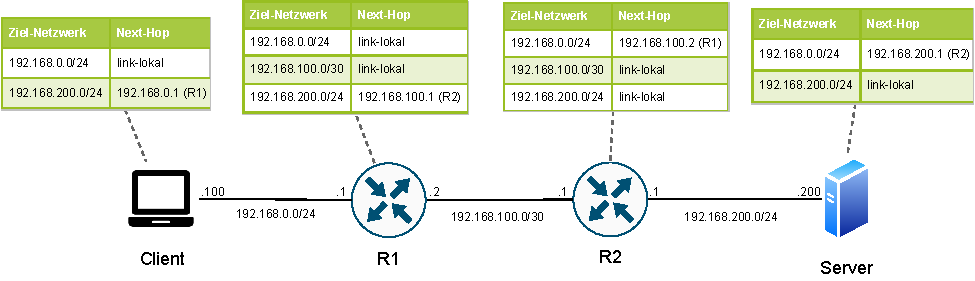
\includegraphics[scale=0.9]{Figures/next_hop_routing_specific_table.pdf}
  \caption{Next Hop Routing}
  \label{grafik: next_hop_routing}
\end{figure}\FloatBarrier
%TC:endignore
Client und Server müssen im Übrigen das Netzwerk 192.168.100.0/30 \textbf{nicht} in ihrer Routing-Tabelle pflegen. Dieses Netzwerk hat ausschließlich eine Relevanz zur Übertragung von Daten zwischen R1 und R2: Man spricht auch von Transfernetzwerken.\\
Dieses Beispiel bringt ein Skalierungsproblem mit sich: Umso mehr Subnetze existieren, in denen Server zu erreichen sind, desto mehr Routen muss der Client in der Routing-Tabelle, u.U. manuell gepflegt, vorhalten. Das gleiche gilt für Server, insofern eine Server-zu-Server-Kommunikation erfolgen soll.\\
In der Praxis sieht man kaum noch Endsysteme (darunter fallen Client und Server), welche mit solchen \textit{spezifischen} Routen arbeiten. Man überlässt die komplexe Verwaltung von Routing-Tabellen den Routern, während die Endsysteme neben der link-lokalen nur noch die \textit{Default}-Route besitzen. In diese Route 0.0.0.0/0 fallen alle Zielnetzwerke, abgesehen vom link-lokalen Subnetz, und sie zeigt immer auf den lokal erreichbaren Router.\\
Das Setzen der Default Route garantiert allerdings nicht, dass ein Ziel auch wirklich erreicht werden kann, z.B. weil es gar nicht existiert oder das Zielnetzwerk nicht in der Routing-Tabelle eines (Next-Hop-)Routers vorhanden ist. Ein Hilfsprotokoll zur Signalisierung von Erreichbarkeit ist dabei das Internet Control Message Protocol (ICMP). Das bekannte Werkzeug \texttt{ping} nutzt Nachrichten in Form von ICMP Echo Request und ICMP Echo Response, um die Erreichbarkeit via IP eines Endsystems zu prüfen.
\begin{figure}[h]
  \centering
  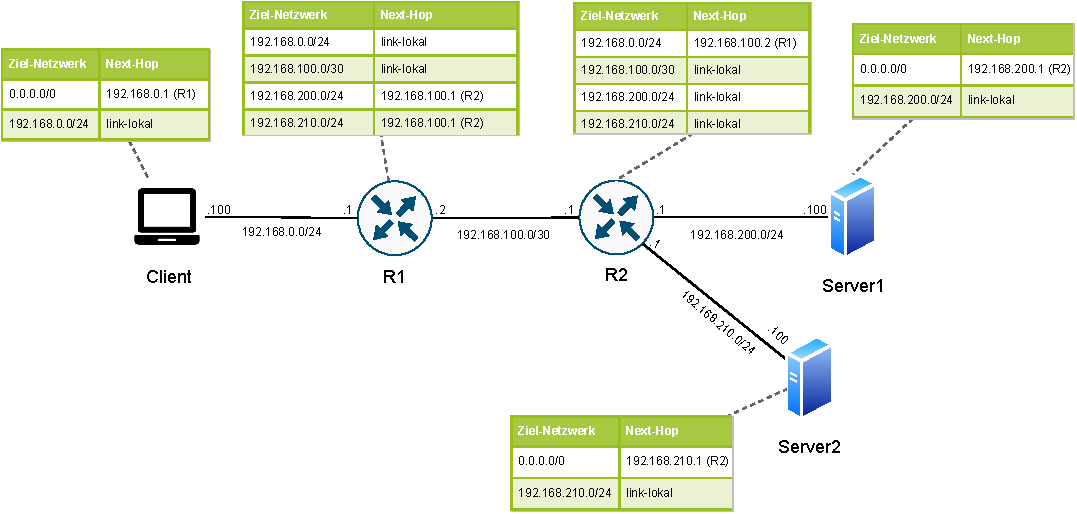
\includegraphics[scale=0.85]{Figures/next_hop_routing_default_route.pdf}
  \caption{Next Hop Routing mit Default Route}
  \label{grafik: next_hop_routing_with_default_route}
\end{figure}\FloatBarrier

Prinzipiell spielen im IPv4-Routing viele weitere Mechanismen eine zentrale Rolle: Zu nennen wären an dieser Stelle bspw. MAC-Adressen (Ethernet), Address Resolution Protocol (ARP), administrative Distanz und Time-To-Live (TTL). Für diese Ausarbeitung haben die Themen allerdings keine besondere Relevanz.\\

\textbf{\underline{Statisches IP-Routing}}\\
Bei nochmaliger Betrachtung der Abbildung \ref{grafik: next_hop_routing_with_default_route} erkennt man zwei Next-Hop Typen: link-lokal und \glqq IP-Adresse\grqq{}. Die link-lokale Route wird automatisch angelegt, sobald eine Netzwerkschnittstelle mit den entsprechenden Adressparametern konfiguriert wird.\\
Routen hingegen, die als Next-Hop eine IP-Adresse beinhalten, müssen entweder als statische oder dynamische Route den Weg in die Routing-Tabelle finden. Statische Routen sind Routen, bei denen ein Administrator Ziel-Netzwerk und Next-Hop manuell auf den Geräten pflegt.\\
Bis zu einer gewissen Netzwerkgröße lassen sich die Routing-Einträge statisch pflegen. Ab größeren Skalierungen mit vielen Routern und Zielnetzwerken wird die Administration jedoch problematisch. So kann es passieren, dass Router in der Konfiguration vergessen werden oder Routing-Einträge fehlen: dies macht eine Weiterleitung dann unmöglich und die Pakete werden verworfen.\\
Weiterhin bieten statische Routen wenig Flexibilität, wenn Verbindungen ausfallen: Es ist zwar möglich, Backup-Routen zu definieren, die zum gleichen Ziel über einen anderen Next-Hop führen mit Hilfe einer schlechteren \textit{Routing-Metrik}. Allerdings kann man nicht alle \textit{Fallback-Szenarien} des Routings vorab durchdenken.

\textbf{\underline{Dynamisches IP-Routing}}\\
IP-Routing auf Basis von dynamischen Routing-Protokollen kann geschilderte Probleme umgehen, indem manuelle Administrationsaufwände verringert bzw. nicht erforderlich werden. Router, die ein dynamisches Routing-Protokoll nutzen, können gegenüber benachbarten Routern Erreichbarkeit für bestimmte Netzwerke signalisieren. Diese Information wird kaskadiert durch das gesamte Netzwerk getragen und es erhalten alle berechtigten Router einer \textit{Routing-Domäne} die Information, \textit{welche} Netzwerke erreichbar sind und \textit{wie} sie erreicht werden können. Auch Fallback-Szenarien sind durch dynamische Routing-Protokolle abgedeckt. Meist werden Backup-Routen schon im Speicher vorgehalten, um bei Ausfall einer Verbindung das Routing zu \textit{schwenken}. Man spricht auch von \textit{Routing-Konvergenz}.

\textbf{\underline{Border Gateway Protocol v4 (BGP)}}\\
Im Folgenden soll das Routing-Protokoll BGP betrachet werden. Dieses ist durch die Public Cloud-Provider vorgegeben, wenn dynamisches Routing gewünscht ist. Es ist ein so genanntes AS-Pfadvektorprotokoll. AS steht dabei für Autonomous System: Ein AS kann als eine administrative \glqq Grenze\grqq{} für eine Gruppe von Routern aufgefasst werden. Tauschen Router per BGP Routing-Informationen aus, spricht man auch von einem \textit{BGP-Peering}. Man unterscheidet an dieser Stelle zwischen internal BGP (iBGP) und external BGP (eBGP): Peerings innerhalb eines AS sind iBGP-Peerings, Peerings über AS-Grenzen hinweg sind eBGP-Peerings. iBGP dient dem Zweck, per eBGP gelernte Routen (\textit{(BGP-)Präfixe}) innerhalb eines AS weiterzutragen.

\begin{figure}[h]
  \centering
  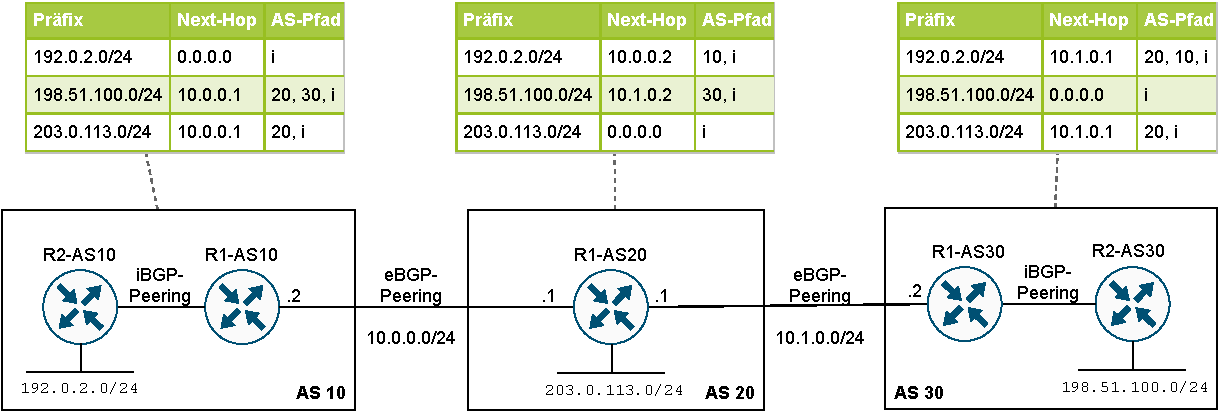
\includegraphics[scale=0.75]{Figures/ebgp_peerings.pdf}
  \caption{Verschiedene AS signalisieren Erreichbarkeit für Präfixe}
  \label{grafik: ebgp_peerings}
\end{figure}\FloatBarrier

Wie man auf der Abbildung \ref{grafik: ebgp_peerings} erkennt, werden drei Präfixe aus drei verschiedenen AS bekannt gemacht. Der AS-Pfad zeigt an, über welche AS ein Präfix erreicht werden kann. \textit{i} steht dabei für internal und stellt den Ursprung des Präfixes dar. Der Pfad wird von rechts (Ursprung) nach links gelesen.\cite{odom2010}\\
\textit{Anmerkung}: R2-AS10 kann mit dem Next-Hop 10.0.0.1 aus der Tabelle nichts anfangen: Dieser ist nur für R1-AS10 erreichbar. Im iBGP nutzt man daher das Attribut \textit{Next-Hop-Self}, womit iBGP-Nachbarn signalisiert wird, dass Next-Hop-Erreichbarkeit für ein Präfix \textit{über einen selbst} gegeben ist.\cite[S.468-471]{odom2010}\\
Die Next-Hop IP für Präfixe anderer AS zeigt bei R2-AS10 somit auf die IP von R1-AS10.

\begin{figure}[h]
  \centering
  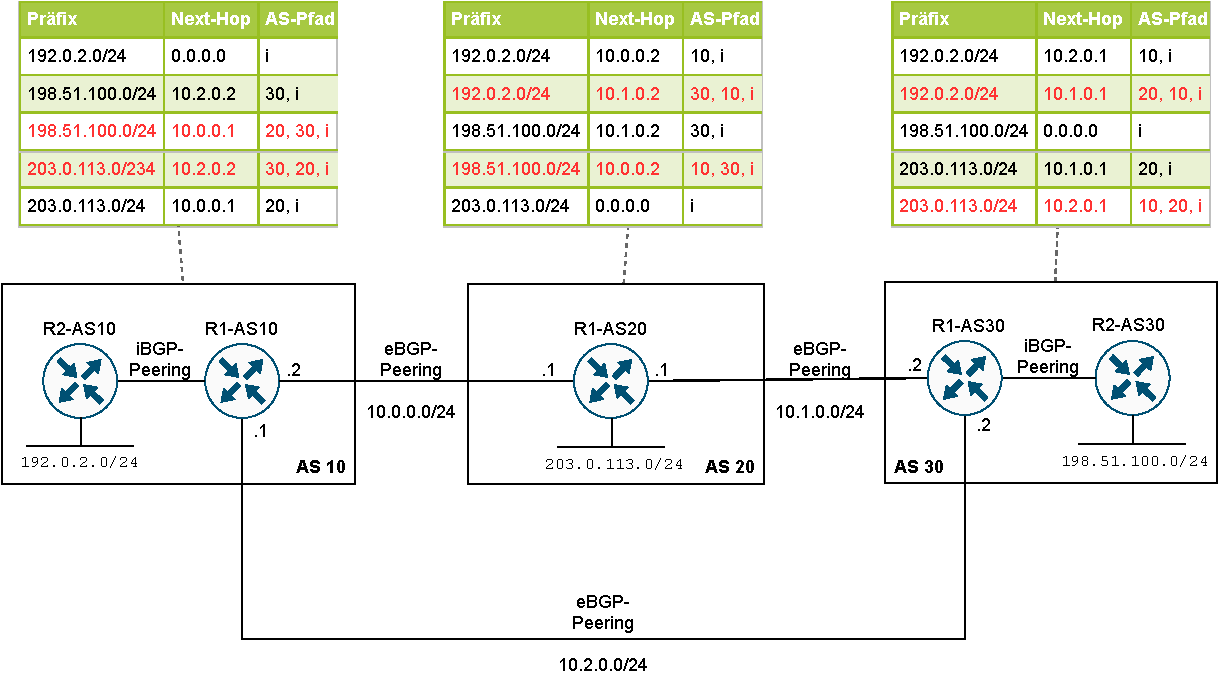
\includegraphics[scale=0.75]{Figures/ebgp_peerings_additional_connection.pdf}
  \caption{Gleicher Grundaufbau wie in Listing \ref{grafik: ebgp_peerings} mit zusätzlicher Verbindung}
  \label{grafik: ebgp_peerings_additional_connection}
\end{figure}\FloatBarrier

In Listing \ref{grafik: ebgp_peerings_additional_connection} wurde noch eine Verbindung zwischen AS 10 und AS 30 hinzugefügt. Damit werden alle Präfixe, bis auf die eigenen, doppelt sichtbar, da sie nun über verschiedene Pfade erreicht werden können. Im Standardfall wird das Präfix mit dem kürzeren AS-Pfad bevorzugt.\\
Die Präfixe mit roter Schrift sind dabei allerdings nicht wertlos. Sie können als Backup-Pfad dienen, falls der bessere Pfad wegfallen sollte. Falls bspw. die Verbindung zwischen AS 10 und AS 30 ausfällt, \textit{konvergiert} das BGP auf allen Routern wieder hin zum Beispiel aus Abbildung \ref{grafik: ebgp_peerings}.\\
BGP-Router ignorieren AS-Pfade, in denen die eigene AS-Nummer bereits vorkommt. Pakete werden dann gemäß RFC 4271 verworfen. Dadurch werden effektiv Routing-Schleifen verhindert\cite{rfc4271}.\\
BGP sieht analog zu RFC 1918-Adressen Bereiche für AS-Nummern vor, die privat, also nicht im Internet, verwendet werden dürfen. Diese Nummern sind in RFC 6996 gelistet und gehen von einschließlich 64512 bis 65534\cite{rfc6996}.

\subsection{Network Address Translation (NAT)}
Grundlegend geht es bei NAT darum, eine IP-Adresse \textit{umzuschreiben}. Dies ist sowohl für die Absender- als auch die Ziel-Adresse möglich. Dies kann verschiedene Gründe haben, oftmals geht es aber darum, IPv4-Adressen einzusparen.\\
Dies ist dem Umstand geschuldet, dass IPv4 nur einen Adressraum von 32 Bit hat, was $2^{32} \approx 4*10^9$ Adressen entspricht. Wenn man dagegen hält, dass die Weltbevölkerung zum Zeitpunkt der Arbeit knapp $8*10^9$ Menschen beträgt und viele Menschen bereits mehr als ein Endgerät besitzen, reicht der Adressraum bei weitem nicht mehr aus \cite{weltbevoelkerung2020dsw}.\\
Langfristig soll IPv6 mit einem Adressraum aus $2^{128}$ Bit IPv4 ablösen, doch selbst im Jahr 2021 fehlt weiterhin die \textbf{vollständige Unterstützung} einiger Hersteller für IPv6. Dies gilt ebenso für Public Cloud-Plattformen.\\
Der häufigste NAT-Mechanismus ist Network Address Port Translation (NAPT). Dabei können $n$ Clients hinter einer einzigen IPv4-Adresse \glqq verborgen\grqq{} und so IP-Adressen eingespart werden. Dafür werden neben der IP-Adresse bspw. noch Information der Transport-Schicht (Layer 4) wie Ports herangezogen, um NAPT-Sessions zuordnen zu können. Ein Router verwaltet diese Sessions in Form einer NAPT-Tabelle. Diese wird notwendig, wenn Rückpakete die verborgenen Clients erreichen sollen.\\
In dieser Ausarbeitung ist, wenn von NAT oder NATting gesprochen wird und keine anderweitigen Aussagen getroffen werden, der NAPT-Mechanismus gemeint.\\
Im Beispiel von Abbildung \ref{grafik: napt} werden drei Clients hinter einem Router geNATtet. Alle eingehenden Pakete werden auf die Quell-IP 10.1.0.1 umgeschrieben und es wird ein neuer Quell-Port vergeben. Wenn nun eine Verbindung von einem Client initiiert wird, sieht der Webserver lediglich die Quell-IP und den Quell-Port des Routers, welche durch das NAT vergeben wurden.\\
Rückpakete vom Webserver zu einem Client werden folgerichtig an den Router adressiert, welcher wiederum in der NAT-Tabelle nachschlägt, um den ursprünglichen Client (interne Absender-IP 10.0.0.x und Quell-Port) herauszufinden. Bevor Pakete also nach intern weitergeschickt werden können, werden sie auf das ursprüngliche Tupel aus Quell-IP und Quell-Port umgeschrieben.\\

\begin{figure}[h]
  \centering
  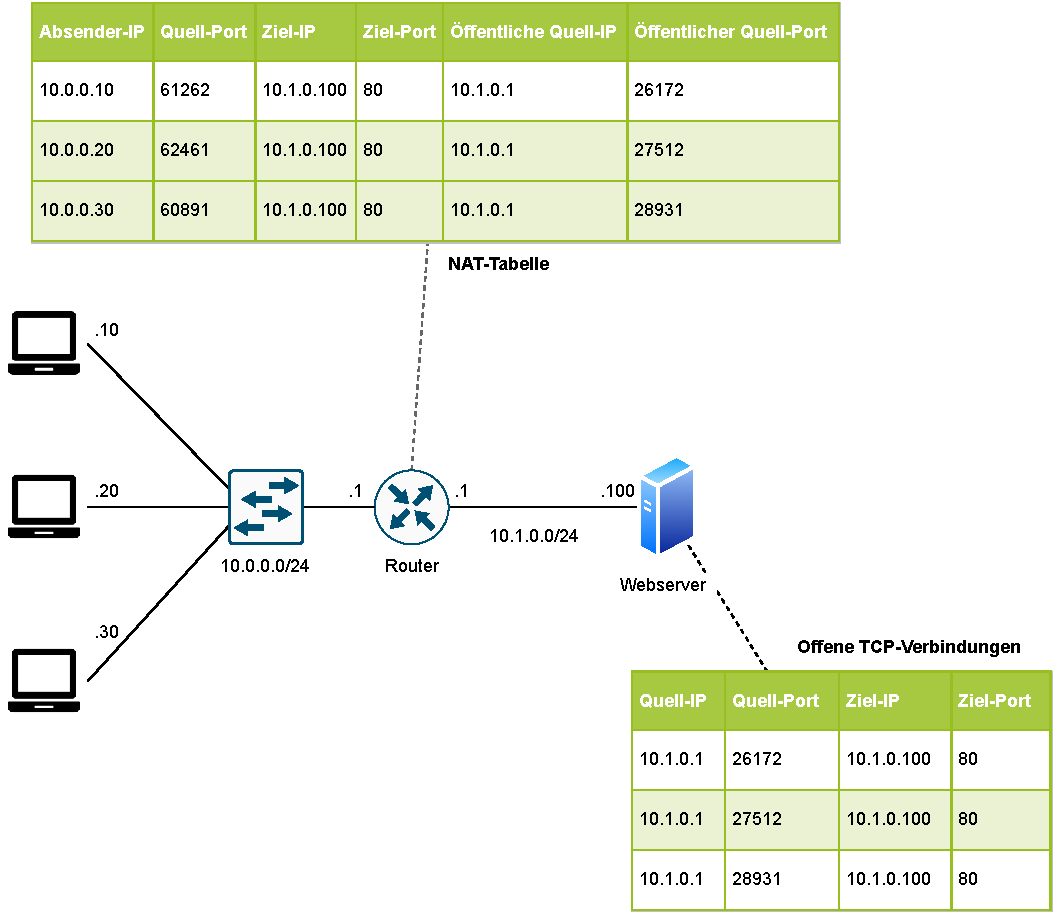
\includegraphics[scale=0.90]{Figures/napt.pdf}
  \caption{Beispiel für Network Address Translation}
  \label{grafik: napt}
\end{figure}\FloatBarrier

NAT\label{nat-bad} verletzt das Prinzip der Ende-zu-Ende-Konnektivität: Findet sich für ein \textbf{vom Webserver kommendes} Paket in der NAT-Tabelle kein Eintrag, wird das Paket verworfen. Dies ist bei einer Client-zu-Server-Kommunikation oftmals kein Problem, da Verbindungen ohnehin vom Client initiiert werden und sich daraufhin ein State in der NAT-Tabelle des Routers befindet.\\
Wenn allerdings eine Client-zu-Client-Kommunikation stattfinden soll, ist man auf aufwändige Mechanismen wie z.B. Hole Punching angewiesen \cite[S.317]{Fall2011}.\\
Auf NAT soll daher in dieser Arbeit verzichtet werden, wenn dies möglich ist und es soll eine vollwertige Ende-zu-Ende-Konnektivität gewährleistet werden.

\subsection{Maximum Transmission Unit / Maximum Segment Size}\label{mtumss}
Die maximale Paketgröße auf einem Netzwerkmedium wird durch die Maxmimum Transmission Unit (MTU) beschrieben. Im Ethernet ist die \textit{Default}-MTU 1500 Byte.\cite[S.86]{Fall2011} Ethernet ist im Internet inzwischen das meistgenutzte Medium, daher haben sich auch hier diese 1500 Byte manifestiert.\\
Da die MTU auf dem Weg vom Empfänger zum Ziel variieren und auch mal geringer als 1500 Byte ausfallen kann, kann ein IPv4-Paket \textit{fragmentiert} werden. Dieser Prozess fordert Rechenzeit für Aufteilung und (Wieder-)Zusammensetzung in Fragmente und kann sich negativ auf die Performance (Latenz und Datendurchsatz) auswirken.\\
Man nutzt optimalerweise Path MTU Discovery oder beeinflusst die Maximum Segment Size für TCP (\glqq MSS-Clamping\grqq{}) bei Initiierung der Verbindung, um Fragmentierung (bestmöglich) zu umgehen.

\subsection{GeoIP}
Mit Hilfe von GeoIP-Datenbanken ist es möglich, den (ungefähren) Standort anhand der Absender-IP-Adresse eines Clients zu bestimmen. Verwendung finden solche Datenbanken häufig bei Internet-Streaming-Anbietern, um Zugriffe auf ein Videoangebot aus dem Ausland zu verhindern. Die Firma MaxMind ist dabei führender Anbieter für solche GeoIP-Datenbanken \cite{maxmind2021geoip}.

\section{Domain Name System (DNS)}\label{DNS}
Das DNS ermöglicht, Server im Internet anhand eines Namens, dem Fully Qualified Domain Name (FQDN), zu erreichen. Somit muss sich ein Benutzer einer Webseite keine IP-Adresse merken, sondern lediglich den dazugehörigen FQDN. Die IP-Adresse wird über die \textit{DNS-Auflösung} herausgefunden. Das DNS ist ein hierarchisches Modell, welches mit Domains arbeitet. Diese unterliegen unterschiedlichen Autoritäten. 
\begin{figure}[h]
  \centering
  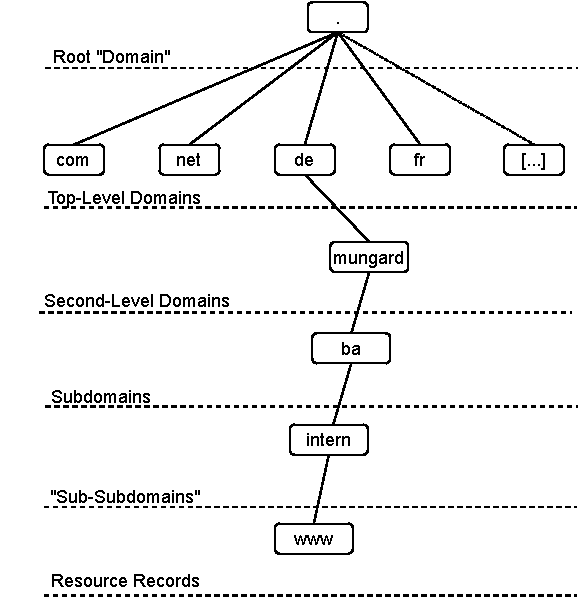
\includegraphics{Figures/dns_autoritative.pdf}
  \caption{DNS-Hierarchie}
  \label{grafik: dns-hierarchy}
\end{figure}\FloatBarrier

Soll z.B. der FQDN www.intern.ba.mungard.de. aufgelöst werden (s. Abb. \ref{grafik: dns-hierarchy}), muss der \textit{Baum} von der Wurzel \glqq .\grqq{} über die Knoten \glqq de\grqq{}, \glqq mungard\grqq{}, ... bis zum Blatt \glqq www\grqq{} durchlaufen werden. Man spricht von einer iterativen Auflösung. Pro Hierarchie-Ebene sind \textit{autoritative Nameserver} verantwortlich für die richtige Delegation des auflösenden Clients.\\
Das Blatt \glqq www\grqq{} wird auch als Resource Record bezeichnet. Für diese Arbeit sind lediglich A-Records relevant, welche FQDN nach IPv4-Adresse auflösen. Viele weitere DNS-Records existieren, z.B. für IPv6-Adressen (AAAA) oder um Mailserver (MX) für eine Domain anzugeben \cite[S.528]{Fall2011}.\\
Ein Beispiel für einen autoritativen Nameserver ist Bind \cite{liu2006dns}. Innerhalb des Nameservers werden Domains anhand von \textit{Zonen(-Dateien)} verwaltet.
\newpage
\subsection{DNS-Resolver}
Clients machen diese iterative Namensauflösung typischerweise nicht selbst, sondern leiten ihre Anfragen an einen DNS-Resolver weiter (\textit{Forwarding}). Dieser sucht \textit{iterativ} zu einem FQDN eine IPv4-Adresse und liefert sie dem Client aus (s. Abb. \ref{grafik: dns-resolver}). Wenn ein Nameserver für eine gesuchte Domain nicht autoritativ ist, wird der Resolver per NS Record weiterdelegiert.\\
Weiterhin kann ein Resolver Einträge \textit{cachen}, um auf erneute Anfragen für gleiche FQDN schneller zu antworten.%Der letzte Punkt eines FQDN, welcher die Root-Domain repräsentiert, wird üblicherweise ausgelassen.
\begin{figure}[h]
  \centering
  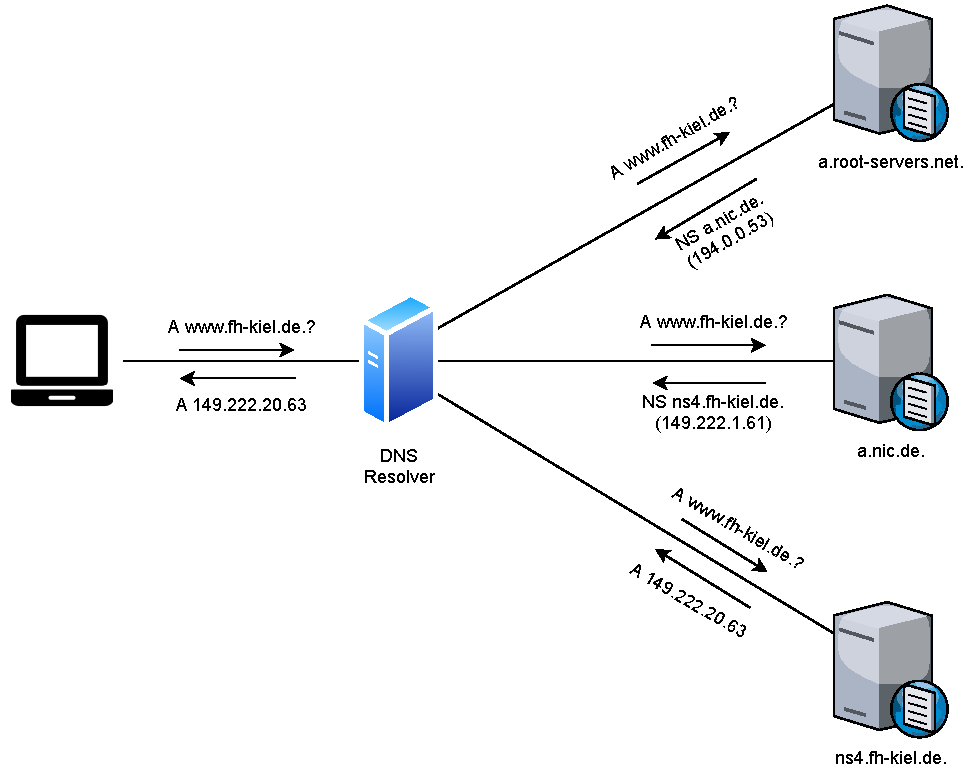
\includegraphics[scale=0.7]{Figures/dns_recursion.pdf}
  \caption{DNS-Resolver}
  \label{grafik: dns-resolver}
\end{figure}\FloatBarrier
%TC:ignore
In Listing \ref{dig-example-fh-kiel} wird ein A-Record für die Domain www01.fh-kiel.de gegen den Resolver von Google (8.8.8.8) mit dem Werkzeug \texttt{dig} aufgelöst.
\begin{listing}[h]
\begin{minted}[breaklines,frame=single]{bash}
$ dig www01.fh-kiel.de @8.8.8.8 | grep -v '^$'
; <<>> DiG 9.11.9 <<>> www01.fh-kiel.de @8.8.8.8
;; global options: +cmd
;; Got answer:
;; ->>HEADER<<- opcode: QUERY, status: NOERROR, id: 11777
;; flags: qr rd ra ad; QUERY: 1, ANSWER: 1, AUTHORITY: 0, ADDITIONAL: 1
;; OPT PSEUDOSECTION:
; EDNS: version: 0, flags:; udp: 512
;; QUESTION SECTION:
;www01.fh-kiel.de.              IN      A
;; ANSWER SECTION:
www01.fh-kiel.de.       21599   IN      A       149.222.20.63
;; Query time: 60 msec
;; SERVER: 8.8.8.8#53(8.8.8.8)
;; WHEN: Tue May 18 22:21:45 CEST 2021
;; MSG SIZE  rcvd: 61
\end{minted}
\caption{DNS-Auflösung für einen A-Record gegen den Resolver von Google}
\label{dig-example-fh-kiel}
\end{listing}\FloatBarrier
%TC:endignore

\subsection{Split DNS}
Split DNS ist die Möglichkeit, verschiedene Resource Records anhand der Absender-IP auszuliefern. Dafür pflegen autoritative Nameserver Access Control Lists (ACL) mit verschiedenen IP-Präfixen, um eine Fallunterscheidung treffen zu können\cite[S.565-567]{Fall2011}. Dies ist z.B. relevant, wenn eine Firma zwischen internen und externen Anfragen unterscheiden muss, um den (richtigen) Zugriff auf Ressourcen zu gewährleisten.

\begin{figure}[h]
  \centering
  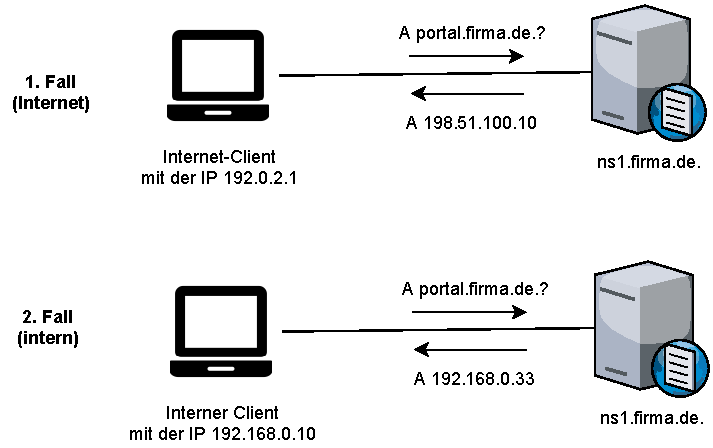
\includegraphics{Figures/dns_split_view.pdf}
  \caption{Split DNS für portal.firma.de.}
  \label{grafik: split-dns}
\end{figure}\FloatBarrier

\subsection{DNS UPDATE}
Die Methode DNS UPDATE ist in RFC 2136 definiert und erlaubt es, autoritative Zonen eines Nameserver zur Laufzeit zu verändern\cite{rfc2136}. Somit müssen keine Zonen-Dateien manuell angepasst werden. Außerdem muss der Nameserver nicht neugestartet werden, um die editierten Zonen-Dateien neu einzulesen.\\
Clients werden über eine ACL ermächtigt, diese Updates zu tätigen. Dabei kann die Absender-IP zur Authentifizierung genutzt werden: Allerdings ist diese Methode unsicher, da sich IPs \textit{spoofen}, d.h. fälschen, lassen\cite[S.70-71]{Fall2011}. Sicherer ist es, mit Hilfe eines vorab ausgetauschten Schlüssels (\textit{Pre-Shared Key}) eine DNS UPDATE-Nachricht zu signieren. Dies passiert mit Hilfe von Transaction Signatures (TSIG) \cite[S.911-914]{Fall2011}.

\section{Virtual Private Network (VPN)}\label{vpn}
VPNs werden genutzt, um private Netzwerke über eine öffentlich genutzte Infrastruktur abbilden zu können. Dies erfolgt zwischen VPN-Endpunkten über gängige Enkapsulierungen, z.B. Generic Routing Encapsulation (GRE), Encapsulating Security Payload (ESP) oder OpenVPN.\\
In Abbildung \ref{grafik: vpn-example} werden Daten von Client A zu Client B über das Internet zwischen Router R1 und Router R2 enkapsuliert. R2 empfängt das Datenpaket, packt es aus und sendet es in der ursprünglichen Form weiter an Client B.\\
Das Diagramm ist dabei nicht spezifisch für eine bestimmte VPN-Technologie. Es können, je nach Technologie, Nutzdaten verschlüsselt werden. 
\begin{figure}[h]
  \centering
  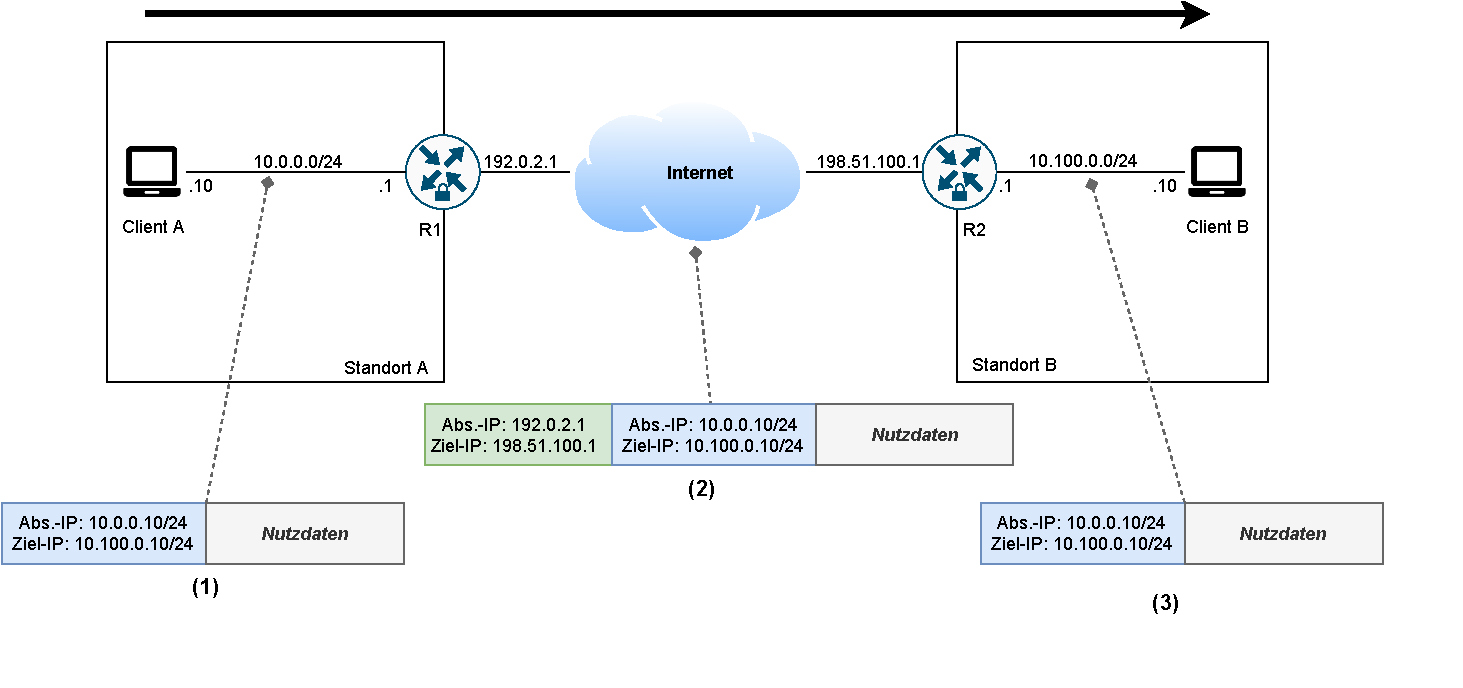
\includegraphics[scale=0.65]{Figures/vpn-example.pdf}
  \caption{Übertragung eines IP-Pakets über einen VPN-Tunnel}
  \label{grafik: vpn-example}
\end{figure}\FloatBarrier

Die in dieser Arbeit verwendeten VPN-Technologien sind IPsec und OpenVPN. IPsec wird u.a. für die Vernetzung von (Cloud-)Standorten, auch Site-to-Site (S2S) genannt, genutzt und arbeitet auf OSI-Schicht 3. Ebenso dient es zur \textit{Einwahl} in (Firmen-)Netzwerke. IPsec wird meist im Geschäftsumfeld genutzt und es exisitieren viele herstellerabhängige Implementationen.\\
OpenVPN ist ein Open Source-Projekt und es nutzt \textit{Transport Layer Security} (TLS) für die verschlüsselte Übertragung von Daten via UDP oder TCP. Das Protokoll ist auf OSI-Schicht 7 zu finden und es wird vor allem für Client-to-Site-Verbindungen genutzt (C2S): Passende Software ist für viele verschiedene Plattformen verfügbar (u.a. Windows, Linux, Mac, Android) und sowohl Client- als auch Server-Applikation sind kostenfrei erhältlich.\\
Angesprochene MTU-Probleme (s. \ref{mtumss}) können sich bei einer getunnelten Verbindung auf Grund des zusätzliches \textit{Overheads} auf Grund der Enkapsulierung zeigen. Eine IP-Fragmentierung sollte optimalerweise verhindert werden.

\section{Cloud}\label{cloud}
Der Cloud-Begriff kann je nach Literatur variieren. Diese Arbeit verweist an dieser Stelle auf die Definition des \textit{National Institute of Standards and Technology (NIST)}. Ebenso werden dort die drei typischen \textit{Cloud Delivery}-Modelle Software as a Service (SaaS), Platform as a Service (PaaS) und Infrastructure as a Service (IaaS) definiert, welche fortan als bekannt vorausgesetzt werden.\cite{mell2011}

\subsection{Public und Private Cloud}
Auch für die so genannten \textit{Cloud \gls{Deployment}}-Modelle wird auf die Definition des NIST verwiesen.\cite{mell2011}\\
Allerdings soll an dieser Stelle auf ein häufiges Missverständnis hingewiesen werden: Eine Private Cloud existiert nicht zwingend \textit{on-premises} einer Organisation, also bspw. im eigenen Rechenzentrum. Sie kann ebenso über Public Cloud-Plattformen abgebildet werden. Allerdings ist die Voraussetzung, dass alle genutzten Ressourcen dann exklusiv für die Organisation zur Verfügung stehen (\textit{exclusive use by a single organization}). Sie werden nicht mit weiteren Parteien geteilt (\textit{open use by the general public}).\\
Die Public Cloud-Provider, welche in dieser Arbeit genutzt werden, sind Amazon Web Services (AWS) und Microsoft Azure. Rechenzentren stehen weltweit zur Verfügung, um eine schnelle und latenzarme Anbindung für die Kunden zu ermöglichen. Eine Private Cloud lässt sich bspw. mit OpenStack abbilden\cite{sefraoui2012openstack}.

\subsection{Multi und Hybrid Cloud}
Eine Multi Cloud vernetzt \textbf{gleiche} Cloud \gls{Deployment}s miteinander, z.B. Public Cloud 	$\leftrightarrow$ Public Cloud oder Private Cloud $\leftrightarrow$ Private Cloud.\\
Bei einer Hybrid Cloud werden unterschiedliche Bausteine zusammengefasst. In dieser Arbeit soll eine Hybrid Cloud aus AWS, Azure (Public) und Private Cloud bereitgestellt (\glqq {Deployment}\grqq{}) werden.

\section{Public Cloud-Netzwerke}\label{public-cloud-networking}
In diesem Kapitel wird näher auf die verschiedenen Netzwerk-\textit{Building Blocks} der Public Cloud-Plattformen AWS und Azure eingegangen. Beide bringen oftmals ähnliche Bausteine mit. Es wird daher stets versucht, im jeweiligen Kontext auf beide Plattformen zugleich einzugehen, um die Grundfunktionalität zu erläutern.
Dieses Kapitel vermittelt lediglich Grundlagen, die für das Verständnis der Use-Cases in Kapitel \ref{Defintion der Use-Cases} und Kapitel \ref{Umsetzung der Use-Cases und Evaluation} notwendig sind. Besonderheiten und Constraints, die sich im Verlauf der Bearbeitung ergeben haben, werden im jeweiligen Use-Case unter \glqq Probleme und Lösungsfindung\grqq{} zusammengefasst.

\subsection{AWS VPC / Azure VNET}
AWS Virtual Private Cloud (VPC) und Azure Virtual Network (VNET) bilden private Netzwerke innerhalb eines Cloud-Mandanten ab. Die hier hinterlegten Präfixe bilden eine Menge an möglichen IP-Adressen innerhalb von VPC und VNET ab. Es können sowohl Public IP-Präfixe als auch IPs nach RFC 1918 benutzt werden. Diese Menge an IP-Adressen wird in AWS \textit{CIDR} bzw. Azure \textit{Address Space} als Container zusammengefasst.\\
AWS gibt /16 als minimale und /28 als maximale Größe des CIDR vor \cite[S.100]{awsug2020}. Azure VNET ist da großzügiger und es darf eine Größe zwischen /8 und /29 gewählt werden\cite[S.10]{Toroman2019}. 
\subsection{Subnets}
Innerhalb von VPC und VNET können Subnets angelegt werden. In diesen Subnets können bspw. virtuelle Maschinen mit IPs ausgestattet werden. Wenn also ein VPC ein CIDR-Präfix von 10.0.0.0/16 besitzt, kann z.B. ein Subnet 10.0.1.0/24 \glqq herausgeschnitten\grqq{} werden. Mit Subnets können weitere Objekte verknüpft werden wie z.B. Route Tables, welche das Routing für das Subnet steuern.

\subsection{Route Tables}
Route Tables ermöglichen es, den Fluss von IP-Pakete innerhalb eines Subnets zu steuern. So können z.B. statische Routen auf Ziele innerhalb eines Subnets angelegt werden. VNET kann dies, wie aus dem klassischen Netzwerk gewohnt, über Next-Hop IPs abbilden. VPC hingegen unterstützt als Next-Hop virtuelle Maschinen (Instances) und Interfaces von virtuellen Maschinen. Es existieren noch weitere spezielle Ziele, die genutzt werden können wie z.B. VPN Gateways, um entfernte Netzwerke zu erreichen.\\
Subnets in Azure erfordern keine Route Tables: Alle Maschinen eines VNET erreichen sich untereinander standardmäßig und erreichen Ressourcen im Internet. Sollte ein granulareres Routing notwendig sein, werden Azure Route Tables erforderlich.\\
Subnets in VPC erhalten immer eine Route Table: Ohne weitere Konfigurationen wird einem Subnet die Main Route Table zugewiesen. Diese kann vorab editiert werden, so dass z.B. kein Internet-Traffic für virtuelle Maschinen möglich ist. \textit{Non-Main} Route Tables können für spezielle Anforderungen erstellt und Subnets zugewiesen werden.

\subsection{Security Groups}
AWS Security Groups (SG) bzw. Azure Network Security Groups (NSG) bilden \textit{stateful Firewalling} ab \cite{wool2006packet}. Dabei können sowohl ingress (eingehende), als auch egress (ausgehende) Firewall-Regeln definiert und darauf basierend Pakete gefiltert werden. Typische Protokolle anhand derer Regeln definiert werden können sind UDP, TCP und ICMP.\\
AWS SGs können einer Instanz zugewiesen werden. Wird keine SG explizit für eine Instanz definiert, kommt eine Default SG zu Einsatz, die vom VPC vorgegeben ist.\\
Azure NSGs können sowohl Subnets als auch VMs direkt zugewiesen werden. NSGs für Subnets wirken sich global für alle VMs eines Subnets aus. Wenn granularer Zugriff auf bestimmte VMs gewünscht ist, nutzt man zusätzliche NSGs \glqq auf\grqq{} den jeweiligen Instanzen.

\subsection{VPN}
AWS bringt in Form von Virtual Private Gateway und Transit Gateway Möglichkeiten mit, IPsec-basierte S2S-Verbindungen zu terminieren. Ersteres kann Verbindungen nur innerhalb eines VPC terminieren. Transit Gateway bietet die Möglichkeit, verschiedene VPCs miteinander zu \textit{peeren}. VPN-Verbindungen können auf Transit Gateway terminiert werden und Pakete, die über VPN reinkommen, können alle gepeerten VPCs erreichen.\\
Azure Virtual network gateway kann analog zu AWS Virtual Private Gateway IPsec-Tunnel in einem VNET terminieren.\\
AWS und Azure ermöglichen innerhalb der Tunnel die Nutzung von BGP, um dynamische Routing-Informationen miteinander auszutauschen.


\section{Automatisierung}\label{automatisierung}

Diverse Automatisierungswerkzeuge ermöglichen es, gewünschte Endzustände von Systemen zu definieren. Mit heutigen Werkzeugen wie z.B. \textit{Ansible} muss ein Administrator wenig Programmiererfahrungen mitbringen und schreibt die gewünschten Parameter in eine Konfigurationsdatei, die zu einem gewünschten Zeitpunkt auf Systemen ausgerollt werden. Viele Probleme wurden bereits von anderen Community-Mitgliedern gelöst. Für komplexere Sachverhalte existieren Plugins.\\
Man muss bei Automatisierungswerkzeugen zwischen \textit{Configuration Management} (CM) und \textit{Provisioning} unterscheiden. Provisioner dienen der grundsätzlichen Erstellung einer Infrastruktur, während CM-Werkzeuge diese Infrastruktur als vorhanden annehmen und weitere Konfigurationen auf den jeweiligen Komponenten tätigen\cite[S.20]{Brikman2019}.\\
Eine Analogie wäre: Provisioner setzen das Haus an eine Straße und das CM macht daraufhin die Innenaustattung. Auf die IT angewendet bedeutet dies, dass Provisioner dafür sorgen, dass Ubuntu-Maschinen aufgesetzt werden und zu erreichen sind. Das CM macht daraufhin Paket-Updates und installiert z.B. einen Apache-Webserver.\\
Es gibt keine eindeutige Linie zwischen den beiden Typen von Werkzeugen. So können viele CM-Werkzeuge auch ein Provisioning von Infrastruktur abbilden, während Provisioner auch grundlegendes Configuration Management leisten können\cite[S.20]{Brikman2019}. Das bereits angesprochene Ansible ist ein CM-Tool mit eingeschränkter Provisioning-Funktionalität.\\
Passende Schnittstellen, z.B. in Form einer REST-API, sind Voraussetzung, um Automatisierungswerkzeuge mit entsprechenden Komponenten nutzen zu können.

\subsection{Terraform}
Das Werkzeug, das hauptsächlich für Automatisierungs-Schritte in dieser Arbeit verwendet wird, ist \textit{Terraform} der Firma Hashicorp. Es ist ein Provisioner mit begrenzten Möglichkeiten für Configuration Management. Es besitzt eine Vielzahl an \textit{Resources}, welche es ermöglichen, Infrastruktur-Komponenten reproduzierbar bereitzustellen. Es wird eine deklarativer Sprachstil genutzt, um gewünschte Zustände der Infrastruktur zu beschreiben. Man spricht auch von \textit{Infrastructure as Code} (IaC).

\textbf{\underline{Provider}}\label{tf-provider}\\
Provider sind die Grundvoraussetzung, um die Automatisierung einer Plattform mit Terraform bewerkstelligen zu können. Sie ermöglichen es, mit entsprechenden Schnittstellen der Anbieter, z.B. REST, zu interagieren. Provider liefern meist diverse \textit{Resources} mit, welche Veränderungen tätigen können und \textit{Data Sources}, welche \glqq lesend\grqq{} auf die Infrastruktur zugreifen, um Informationen zurückzuliefern. Diese Informationen können dann anderen \textit{Modulen} zur Verfügung gestellt werden.\cite{Brikman2019}\\
Terraform arbeitet stateful: Nach jedem \texttt{terraform apply}, welches zur Erstellung der gewünschten Infrastruktur führt, werden Referenzen aller Infrastrukturkomponenten in der Datei \underline{terraform.tfstate} gespeichert: Ein erneuter Aufruf von \texttt{terraform apply} würde, insofern keine Konfigurationsänderungen gemacht wurden, die Infrastruktur so belassen und sie nicht nochmals bereitstellen bzw. erweitern. Per \texttt{terraform destroy} kann die Infrastruktur wieder zurückgebaut werden.\\
In Listing \ref{tf-aws-provider-example} wird der Provider \textit{aws} in einer spezifischen Version eingebunden. Der Constraint \glqq $\sim$>\grqq{} sorgt dafür, dass nur Versionen des Providers innerhalb des 3.35.x Branches benutzt werden (\glqq Minor Patches\grqq{}).
%TC:ignore
\begin{listing}[h]
\begin{minted}[breaklines,frame=single]{tf}
terraform {
    required_providers {
        aws = {
            source = "hashicorp/aws"
            version = "~> 3.35.0"
        }
    }
}
\end{minted}
\caption{Terraform AWS Provider}
\label{tf-aws-provider-example}
\end{listing}
%TC:endignore

\textbf{\underline{Resources}}\\
Resources erstellen Infrastuktur-Komponenten und statten diese mit den richtigen Parametern aus. In Listing \ref{deployment_aws_tf} wird ein VPC mit dem CIDR-Block 10.0.0.0/16 und ein darunterliegendes Subnet 10.0.1.0/24 erstellt.
%TC:ignore
\begin{listing}[h]
\begin{minted}[breaklines,frame=single]{tf}
resource "aws_subnet" "example_subnet" {
    vpc_id            = aws_vpc.example_vpc.id
    cidr_block        = "10.0.1.0/24"
    availability_zone = "eu-central-1"
}
resource "aws_vpc" "example_vpc" {
    cidr_block = "10.0.0.0/16"
}
\end{minted}
\caption{Deployment der Resources \glqq example\_vpc\grqq{} und \glqq example\_subnet\grqq{}}
\label{deployment_aws_tf}
\end{listing}
%TC:endignore
Dabei zeigt sich auch der deklarative Aspekt von Terraform. Die Resource \glqq aws\_subnet\grqq{} mit dem Namen \glqq example\_subnet\grqq{} kommt als erstes im Code vor, referenziert jedoch das VPC \glqq example\_vpc\grqq{}. Durch diese impliziete Abhängigkeit wird die Resource \glqq example\_vpc\grqq{} als erstes erstellt. Man beschreibt also, \textit{was} benötigt wird. \textit{Wie} und in welcher Reihenfolge das Rollout gemacht wird, obliegt Terraform.

\textbf{\underline{Module}}\\
Terraform Module sind \textit{Container}, die mehrere Resources in *.tf-Dateien zusammenfassen \cite{tfmodule2021}. Es ist zwar möglich, alle notwendigen Resources in einer einzigen *.tf-Datei zu konfigurieren, allerdings ist es \textit{best practice}, verschiedene Resources der Übersichtlichkeit wegen aufzuteilen und in einer geeigneten Ordnerstruktur unterzubringen. Die jeweiligen Dateien innerhalb eines Ordners heißen dann \underline{main.tf}. Um Attribute an andere Module weiterzugeben, werden \textit{Outputs} genutzt. 

\textbf{\underline{Data Sources und Outputs}}\\
Data Sources führen keine Änderung herbei, sondern werden genutzt, um detaillierte Informationen zu Infrastruktur-Komponenten zurückzugeben oder um etwas zu finden. In Listing \ref{data-source-find-output-id} wird nach einem Amazon Machine Image (AMI) für Ubuntu gesucht. Die ID (image\_id) für das \textit{most recent} Release kann per Output an andere Module weitergegeben werden. Diese können die ID dann z.B. nutzen, um per Resource eine virtuelle Maschine mit dem gewünschten Ubuntu-Image bereitzustellen.
%TC:ignore
\begin{listing}[h]
\begin{minted}[breaklines,frame=single]{tf}
data "aws_ami" "ubuntu" {
  most_recent = true
  filter {
    name   = "name"
    values = ["ubuntu/images/hvm-ssd/ubuntu-focal-20.04-amd64-server-*"]
  }
  filter {
    name   = "virtualization-type"
    values = ["hvm"]
  }
  owners = ["099720109477"] # Canonical
}
output "ubuntu_ami_id" {
  value = data.aws_ami.ubuntu.image_id
}
\end{minted}
\caption{Die Data Source \glqq ubuntu\grqq{} sucht nach dem passenden Ubuntu Image und Output macht die ID global für andere Module verfügbar}
\label{data-source-find-output-id}
\end{listing}\FloatBarrier
%TC:endignore
\subsection{IP Address Management (IPAM)}
Ein IPAM ist wichtig, insofern die Adressverwaltung automatisiert werden soll. Statisch konfigurierte CIDR-Blöcke im Code sorgen für eine schlechte Wiederverwendbarkeit und Skalierbarkeit von Modulen: IP-Blöcke müssten dann jedes Mal händisch reserviert und in den gewünschten Modulen untergebracht werden.\\
Einfacher ist es, im Modul lediglich festzulegen, welche Subnetzgröße erforderlich ist: ein IPAM gibt dann den nächsten freien Block in der passenden Größe zurück. Es wird lediglich ein großer Block vorreserviert, aus dem die freien Blöcke entnommen werden können.

\begin{figure}[h]
  \centering
  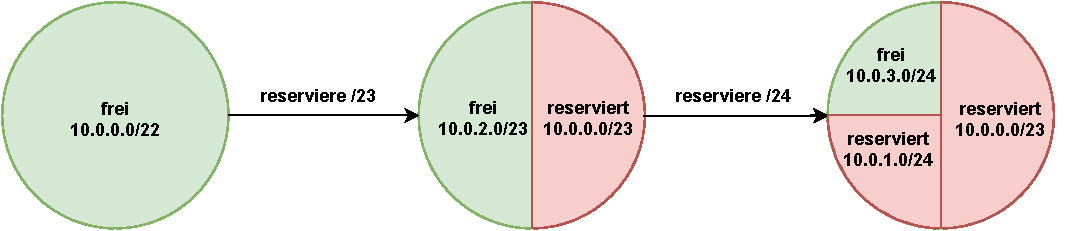
\includegraphics[scale=0.8]{Figures/ipam_cake.pdf}
  \caption{IPAM-Reservierung von CIDR-Blöcken}
  \label{grafik: ipam_ip_reservation}
\end{figure}\FloatBarrier

% \include{Chapters/02_Recherche_und_Auswahl_der_Komponenten}
\chapter{Definition der Use Cases} \label{Defintion der Use-Cases}
In diesem Kapitel werden die Use Cases für ein Hybrid Cloud-\gls{Deployment} vorgestellt und näher erläutert. Es findet eine Vorauswahl über geeignete technische Komponenten statt, welche anschließend in Kapitel \ref{Umsetzung der Use-Cases und Evaluation} genutzt werden. Weiterhin werden messbare Evaluationskriterien für eine erfolgreiche Umsetzung genannt. Bei Vorauswahl und Evaluationskriterien handelt es sich um in der Praxis übliche Anforderungen im Unternehmensumfeld. Grundlegende Kenntnisse v.a. über IPv4(-Routing), \gls{VPN} und Building Blocks der Public Cloud-Plattformen aus dem vorangegangenen Kapitel \ref{Technische_Grundlagen} werden vorausgesetzt.

\section{Use Case 1: Basis Deployment mit Ende-zu-Ende-Konnektivität}\label{base-deployment}
Es wird ein Basis \gls{Deployment} benötigt, um eine grundlegende Integration in die Firmeninfrastruktur zu ermöglichen. So ist die Grundannahme, dass der Kunde bereits Rechenressourcen in Selbstverwaltung (\glqq Private Cloud\grqq{}) besitzt. Weiterhin hat die Integration von Public Cloud-Diensten noch gar nicht oder nur testweise stattgefunden: Es wurden ein paar Maschinen hochgefahren und bestimmte Internetdienste installiert. Über eine tiefergehende Koppelung mit bestehender Infrastruktur hat der Kunde bisher keine Überlegungen angestellt.\\
Eine Hybrid Cloud besteht, wie bereits beschrieben, aus Public und Private Cloud. Da mit den beiden Public Clouds AWS und Azure gearbeitet wird, wäre hier bereits eine Fallunterscheidung notwendig: Private Cloud $\leftrightarrow$ Azure bzw. Private Cloud $\leftrightarrow$ AWS. Um sich diese Fallunterscheidung sparen zu können, soll ein Dreieck ausgerollt werden, bei dem jeder Punkt eine Cloud-Plattform darstellt.
Optimalerweise wird durch dieses \gls{Deployment} auch die Redundanz erhöht: Fällt eine Verbindung aus bspw. zwischen AWS und Azure, so können Datenpakete weiterhin über die Private Cloud geroutet werden.
Der Use Case soll als Grundaufbau für alle weiteren Use Cases dienen und eine Ende-zu-Ende-Konnektivität für alle Teilnehmer garantieren. Das Dreieck aus AWS, Azure und Private Cloud (s. Abb. \ref{grafik:Use-Case-1_Basis_Deployment}) wird fortan als \textit{Backbone} bezeichnet.

\begin{figure}[h]
  \centering
  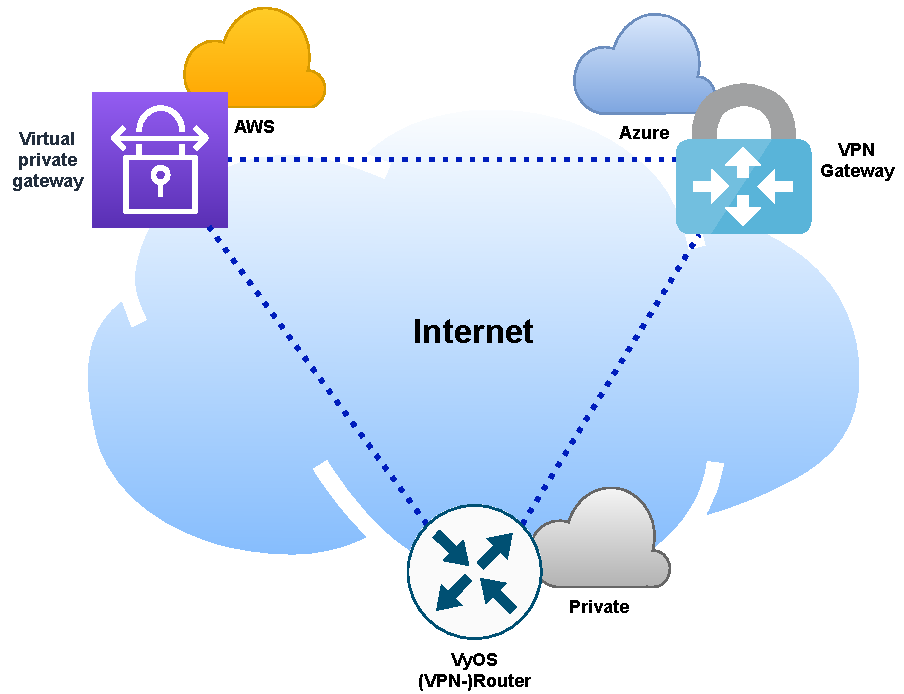
\includegraphics{Figures/Use-Case-1_Basis_Deployment.pdf}
  \caption{Use Case 1: Dreiecks-Topologie für die Hybrid-Cloud (\glqq Backbone\grqq{})}
  \label{grafik:Use-Case-1_Basis_Deployment}
\end{figure}\FloatBarrier

\subsection{Vorauswahl geeigneter technischer Komponenten}
AWS und Azure bieten auf ihren Plattformen Unterstützung für Route-Based \gls{IPsec}-Tunnel\cite[S.32]{awsvpn2021}. Darüber kann eine virtuelle Punkt-zu-Punkt zwischen zwei Standorten hergestellt werden und es kann innerhalb der Tunnel \gls{BGP} gesprochen werden, um ein dynamisches Routing zu ermöglichen\cite[S. 18]{AlShawi2020} \cite[S. 74-79]{Toroman2019}. Gleichzeitig werden übertragene Daten verschlüsselt und dadurch Integrität und Vertraulichkeit geschützt.\\
Das dynamische Routing bietet den Vorteil, dass IPv4-Routen nicht manuell bei allen Gateways des Netzwerks bekannt gemacht werden müssen: Sobald ein Teilnehmer ein neues Netzwerk kennt, wird dies via \gls{BGP} den restlichen Teilnehmern bekannt gegeben.\\
Für das automatisierte \gls{Deployment} der Infrastruktur eignet sich Terraform der Firma Hashicorp. Es besitzt eine Vielzahl an \textit{Resources} (u.a. Azure und AWS), welche es ermöglichen, Infrastrukturkomponenten \textit{reproduzierbar} bereitzustellen.\\
Darüber hinaus wird ein \gls{IPAM} benötigt zur IPv4-Adressverwaltung. Die automatische Zuteilung von Adressbereichen darf nicht dazu führen, dass Adressbereiche mehrfach verteilt werden oder sich Adressbereiche überlappen. Gewählt wurde hier das Werkzeug phpIPAM\cite{phpipam2020}: Es lässt sich sehr gut mit Terraform integrieren, da ein entsprechender Provider zur Verfügung steht\cite{phpipamtf2020}.\\
Die \gls{VPN-Gateway}s, die das Backbone aufspannen, sind mit \textit{Virtual private gateway} bei AWS und \textit{VPN Gateway} bei Azure gesetzt. Dies sind die typischen \textit{Building-Blocks}, die von den Cloud-Providern für \gls{VPN}-Verbindungen angeboten werden. Nur wenn sich im Laufe der Arbeit herausstellen sollte, dass diese Systeme nicht interoperabel sein sollten, wird versucht, Alternativen zu finden.\\
Als Router, der die Private Cloud repräsentiert, wurde ein VyOS Router gewählt. Dieser steht als Open Source zur Verfügung, es gibt allerdings auch bezahlten Support für Produktionsumgebungen. Der Router hat \gls{IPsec}- und \gls{BGP}-Unterstützung und besitzt ein Command Line Interface (CLI), über das Konfigurationen getätigt werden können. Eine REST-API steht ebenso zur Verfügung, aber diese ist zum Stand der Bachelor-Arbeit \textit{cutting edge} und wenig dokumentiert\cite{vyosapi2021}. Ein nativer Terraform Provider steht nicht zur Verfügung.\\
Es soll pro Public Cloud eine virtuelle Maschine bereitgestellt werden, um die Ende-zu-Ende-Konnektivität zwischen den Standorten zu verifizieren.
Die Annahme ist, dass der VyOS-Router, das \gls{IPAM} und eine virtuelle Maschine zum Testen in der Private Cloud bereits vorhanden sind. Diese Komponenten sind nicht Teil des (Terraform-)Deployments. Allerdings müssen Konfigurationsänderungen zum \gls{Deployment} geschehen.\\
Prinzipiell lassen sich viele Router-Modelle nutzen, insofern die Unterstützung für genannte Techniken (Route-based \gls{IPsec}, \gls{BGP}) vorhanden ist, bspw. CSR 1000V der Firma Cisco\cite{Durai2016}. Der offene VyOS Router bietet den Vorteil, dass keine Lizenzen für die Nutzung hinterlegt werden müssen, was in vielen Fällen manuelle Konfigurationen erfordert. Außerdem hätten erst einmal passende Lizenzen beschafft werden müssen, was u.U. zu Verzögerungen der Arbeit geführt hätte.
\subsection{Evaluationskriterien}\label{eval-kriterien-uc1}
Nach der Umsetzung wird evaluiert, ob das \gls{Deployment} folgender Kriterien erfolgreich war:
\begin{enumerate}
    \item IPv4-Adressbereiche werden im \gls{IPAM} reserviert und mit AWS \gls{VPC} und Azure \gls{VNET} assoziiert. Test-Szenario: Zur Verifizierung werden die reservierten Adressbereiche mit den assoziierten verglichen.
    \item \gls{IPsec}-Verbindungen werden zwischen allen \gls{VPN-Gateway}s aufgebaut. Test-Szenario: Dies kann mit einem Blick in die verschiedenen \textit{Dashboards} der Cloud-Plattformen bzw. CLI-Kommando (VyOS) verifiziert werden.
    \item \gls{BGP}-Sessions werden etabliert und Präfixe zwischen den Teilnehmern ausgetauscht. Die Routen müssen in der Routing-Tabelle sichtbar sein. Test-Szenario: Eine Testmaschine pro Cloud-Standort und Ping-Tests zwischen den Standorten veranlassen.
    \item Die Präfixe sollten im Normalfall über verschiedene \gls{AS}-Pfade sichtbar sein. Nur bei Verbindungsverlust sind Präfixe ausschließlich über einen \gls{AS}-Pfad zu sehen. Test-Szenario analog zu Punkt 2.
    \item Verifizierung der Ende-zu-Ende-Konnektivität und einfache Bandbreitenmessungen. Test-Szenario: Ping-Tests und iPerf3-Messungen zwischen den Standorten.
\end{enumerate}

\section{Use Case 2: \gls{Roadwarrior}-VPN}
In diesem Use-Case soll erarbeitet werden, inwiefern sich Mitarbeiter via VPN - im Folgenden \gls{Roadwarrior} genannt - mit den zuvor ausgerollten Cloud-Infrastrukturen verbinden können. Ralf Spenneberg definiert diesen Begriff wie folgt:\\
\glqq Der Begriff \gls{Roadwarrior} bezeichnet Personen, die mit unbestimmter IP-Adresse auf ein \gls{VPN-Gateway} zugreifen wollen. Typischerweise handelt es sich hierbei zum Beispiel um Außendienstmitarbeiter, die von unterwegs Zugriff auf die Datenbanken ihres Mutterunternehmens benötigen. Aber auch alle anderen Konstellation, bei denen Rechner mit dynamischen IP-Adressen eine VPN-Verbindung mit einem \gls{VPN-Gateway} aufbauen möchten, sind denkbar. Hierbei ist die Anzahl der \gls{Roadwarrior} nicht beschränkt. Theoretisch und auch praktisch sind mehrere Hundert gleichzeitiger Tunnel möglich.\grqq{} \cite[S. 199]{Spenneberg2010}\\
Gerade die Corona-Krise hat das Ausweichen auf das Home-Office für einige Branchen unverzichtbar gemacht. Einige prophezeien bereits eine neue Arbeitswelt \textit{New Work}, die \glqq flexible Arbeitsgestaltung, zum Beispiel durch Vertrauensarbeitszeit und -orte sowie Verzicht auf standardisierte Kernarbeitszeiten\grqq{} mit sich bringt \cite{Umbs2020}.
Klassischerweise verbindet sich der \gls{Roadwarrior} mit dem Hauptstandort, um von dort aus weitere interne Ressourcen zu erreichen - in diesem Falle die Private Cloud. Dieses klassische Design bringt insbesondere unter der Annahme, dass sich Dienste in die Cloud verlagern lassen, diverse Probleme mit sich:
\begin{itemize}
\item Der Hauptstandort muss Bandbreite für alle $n$ \gls{Roadwarrior} zur Verfügung stellen. V.a. zu Beginn der Corona-Krise durften viele Unternehmen und öffentliche Einrichtungen erfahren, dass sie hier zu schwach aufgestellt sind \cite{tufreiberg2021}.
\item Der Hauptstandort ist u.U. weit entfernt. Der Mitarbeiter nimmt auf Grund von hohen Latenzen und eventuellen Paketverlusten eine schlechte Applikations-Performance wahr. Dazu wird oftmals über Smartphone-Hotspot, Hotel-WLAN, o.ä. gearbeitet, welche häufig eine unterdurchschnittliche Internetanbindung anbieten.
\item Latenzen erhöhen sich zusätzlich, falls bestimmte Applikations-Server gar nicht am Hauptstandort vorhanden sind, z.B. weil sie in die Public Cloud verlagert wurden.
\end{itemize}
Optimalerweise wird das Design also diese genannten Punkte in Angriff nehmen:
\begin{itemize}
\item Ein Load Balancing der Bandbreiten wird ermöglicht, indem $n$ \gls{Roadwarrior} über $m$ Clouds verteilt werden.
\item Der \gls{Roadwarrior} verbindet sich im günstigsten Fall mit dem Standort, der die geringste Entfernung zu ihm aufweist.
\item Häufig genutzte Applikationen sind am jeweiligen Cloud-Standort, mit dem sich der \gls{Roadwarrior} verbunden hat, verfügbar, um eine gute Usability für den Anwender zu gewährleisten.
\item Weiterhin sollen genannte Maßnahmen für den Anwender möglichst transparent und ohne manuelle Interaktion erfolgen. Er soll keine Wahl haben, mit welchem Cloud-Standort er sich zu verbinden hat: Die Annahme ist, dass dieser über geeignete Automatisierungsmechanismen mit dem \textit{besten} Standort verbunden wird.
\end{itemize}
Das Szenario baut auf Use-Case 1 auf. So wird weiterhin von dem Backbone-Grundaufbau ausgegangen. Es soll gezeigt werden, wie ein \gls{Roadwarrior}-Setup aufgebaut werden kann, bei dem sich der jeweilige Mitarbeiter mit dem nächstgelegen \textit{Hop} verbindet, um die beste Performance erreichen zu können. Weiterhin soll an jedem Cloud-Standort ein (interner) Server stehen, welcher einen internen Netzwerk-Dienst anbietet. Das Ziel ist es, dass ausschließlich der Server genutzt wird, der an dem Standort zur Verfügung steht. Ansonsten würden sich der Latenzgewinn durch die nahe VPN-Gegenstelle durch die \textit{interne} Latenz wieder aufheben.\\
Die Infrastruktur-Komponenten aus Use-Case 1 werden als vorhanden und funktionierend angenommen und in Abbildung \ref{grafik:Use-Case-2_Vereinfacht} nicht mehr dargestellt. Die \gls{Roadwarrior}-\gls{Client}s verbinden sich immer mit dem nächstgelegenen \gls{VPN-Konzentrator}.
\begin{figure}[h]
  \centering
  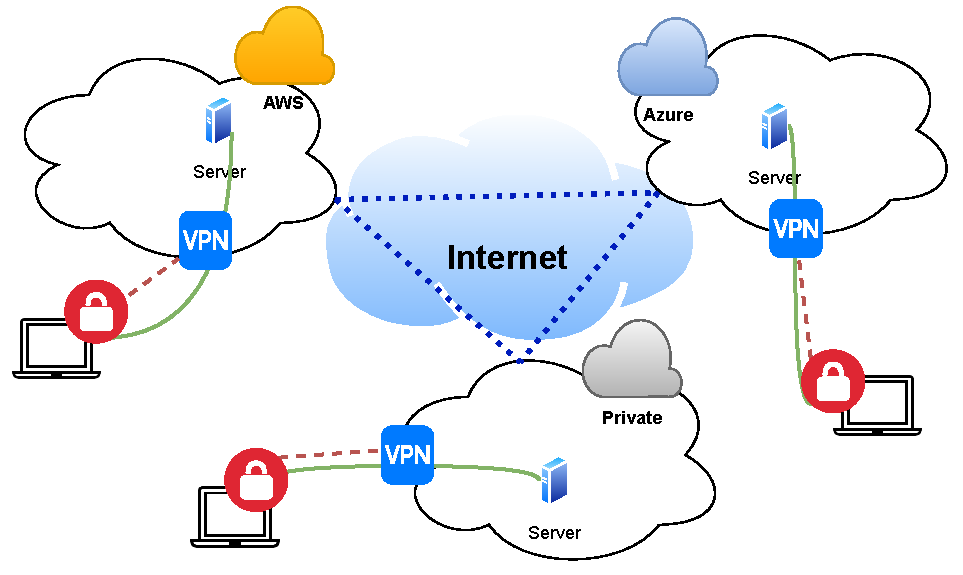
\includegraphics[scale=0.75]{Figures/Use-Case_2_Vereinfacht_1.pdf}
  \caption{Use-Case 2: \gls{Roadwarrior}}
  \label{grafik:Use-Case-2_Vereinfacht}
\end{figure}\FloatBarrier

\subsection{Vorauswahl geeigneter technischer Komponenten}\label{uc1-vorauswahl}
Zur Terminierung der \gls{Roadwarrior}-\gls{Client}s muss pro Cloud-Standort ein \gls{VPN-Konzentrator} zur Verfügung stehen. Mit \textit{\gls{Client} VPN Endpoint} (AWS) bzw. \textit{Point-to-site} Azure bieten bereits Lösungen, um \gls{Roadwarrior}-\gls{Client}s zu terminieren. Nach längerer Evaluation dieser Building Blocks erwiesen sich diese Lösungen für das Ziel der Arbeit als nicht tauglich:
\begin{itemize}
\item Bei AWS werden \gls{\gls{Client}-to-Site}-Verbindungen eingehend geNATted (\textit{NAT Masquerading}). Damit sind alle \gls{Client}s intern mit der gleichen Absender-IP zu sehen. Dies verletzt den Anspruch der Arbeit, eine Ende-zu-Ende-Konnektivität zu ermöglichen.
\item Obwohl Azure als auch AWS OpenVPN für \gls{Roadwarrior}-VPNs benutzen, sind die \gls{\gls{Client}-to-Site}-Konfigurationen nicht \glqq deckungsgleich\grqq{} zu bekommen. Um den sich mit dem nächstgelegenen \gls{VPN-Konzentrator} zu verbinden, wäre eine manuelle Interaktion des Benutzers notwendig, was mit den Evaluationskriterien nicht vereinbar ist. Weiterhin kann der Benutzer nicht immer wissen, wo der nächstgelegene Standort ist. Man kann nicht von jedem Mitarbeiter tiefe Kenntnisse der Netzwerktopologie abverlangen.
\end{itemize}
AWS benutzt bspw. eine \textit{remote-random-hostname}-Direktive (s. Listing \ref{ovpn-client-config-remote}), welche dafür sorgt, dass bei Verbindungsversuch eine Zufallszeichenkette an den Domainnamen angehangen wird, um DNS Caching zu verhindern.
%TC:ignore
\begin{listing}[h]
\begin{minted}[breaklines,frame=single]{bash}
$ grep remote *-client-vpn.ovpn
aws-client-vpn.ovpn:remote cvpn-endpoint-08345.prod.clientvpn.eu-central-1.amazonaws.com 443
aws-client-vpn.ovpn:remote-random-hostname
aws-client-vpn.ovpn:remote-cert-tls server
azure-client-vpn.ovpn:remote azuregateway-61820068.vpn.azure.com 443
azure-client-vpn.ovpn:remote-cert-tls server

\end{minted}
\caption{Auszüge aus den OpenVPN-\gls{Client}-Konfigurationen für AWS und Azure.}
\label{ovpn-client-config-remote}
\end{listing}\FloatBarrier
%TC:endignore
Weiterhin sind die unterschiedlichen Authentifizierungsmechanismen nur schwierig miteinander zu kombinieren. Auch hier wäre eine Benutzerinteraktion notwendig.\\
Daher wurde für weitere Überlegungen von den offiziellen Building-Blocks abgesehen und entschieden, pro Standort einen eigenen OpenVPN-Server hochzufahren: OpenVPN ist freie Software und man muss sich daher nicht mit Lizenzierungen beschäftigen analog zu VyOS.\\
Aus den Erfahrungen aus Use-Case 1 wurde dafür ebenso die Router-Distribution VyOS gewählt. Diese kann nicht nur für \gls{Site-to-Site}-Tunnel genutzt werden, sondern kann auch für \gls{\gls{Client}-to-Site}-Tunnel terminieren, um den Zugang für \gls{Roadwarrior} zu ermöglichen.\\
Denkbar wäre ebenso eine simple Linux-Distribution mit dem Paket OpenVPN: VyOS bietet den Vorteil, dass sich die notwendigen Konfigurationen ebenso über CLI erledigen lassen und somit per Terraform-Template \textit{automatisiert} ausgebracht werden können\cite{vyosopenvpn2021}. VyOS ist im AWS als auch im Azure Marketplace zu beziehen.\\
Ein Problem ergibt sich aus der Authentifizierung und Autorisierung der \gls{Roadwarrior}-\gls{Client}s. Wenn Protokolle wie RADIUS\cite{rfc2865} als Authentifizierungsmechanismus mit Benutzerkennung und Passwort, muss man entweder
\begin{enumerate}[label=(\alph*)]
\item \label{radius-decentralized} einen zentralen RADIUS-Server pro Standort verwalten oder
\item \label{radius-centralized} einen zentralen RADIUS-Server für alle Standorte zur Verfügung stellen.
\end{enumerate}
\ref{radius-decentralized} bringt ein Skalierungsproblem mit sich: So müssen bspw. Benutzerkennungen und Passwörter lokal auf allen Systemen gepflegt werden, was die Komplexität des Use-Cases deutlich erhöhen würde und auch in Realität schwierig zu warten wäre. Mit \ref{radius-centralized} hätte man einen Single-Point-of-Failure, scheidet also auch aus. Hätte der \textit{zentrale} Authentifizierungsserver ein technisches Problem, wären alle \gls{VPN-Konzentrator}en betroffen und \gls{Roadwarrior} könnten sich nicht mehr einwählen.\\
Lightweight Directory Access Protocol (LDAP)\cite{rfc4511} als verteilte Datenbank wäre eine Lösung für genannte Probleme: man müsste pro Standort einen LDAP-Server bereitstellen und durchgehend mit allen weiteren LDAP-Servern synchronisieren. Als Authentifizierungsmechanismus könnte man dann bspw. RADIUS\cite{rfc2865} oder gleich LDAP benutzen. \textit{Windows Domänen Controller} implementieren den LDAP-Verzeichnisdienst in Form von \textit{Active Directory} und wären ein Beispiel für solch ein verteiltes Szenario.\cite[S.603-604]{Tanenbaum2003}\\
In dieser Arbeit wird von der Implementation abgesehen, da die Komplexität deutlich erhöht und es für den Proof-of-Concept an sich keine gewinnbringenden Erkenntnisse liefern würde.\\
Der Lösungsansatz wäre an dieser Stelle, auf eine Zertifikat-basierte Authentifizierung zu setzen. Eine Publik-Key-Infrastruktur benötigt zur Authentifizierung keine Verbindungen zu anderen (Authentifizierungs-)Services. Es reicht, auf dem VPN-Server vertrauenswürdige Root-Zertifikate zu hinterlegen. Diese \textit{vertrauenswürdigen Stellen} signieren mit dem privaten Schlüssel dann die Zertifikate der \gls{Roadwarrior}-\gls{Client}s, wodurch das Vertrauensverhältnis zwischen VPN-Server und -\gls{Client} hergestellt ist.\\ 
Auf Prüfung der Gültigkeit von Zertifikaten mittels Certificate Revocation Lists (CRLs) bzw. Online Certificate Status Protocol (OCSP) wird in dieser Arbeit verzichtet. Sie ist aber prinzipiell möglich mit der serverseitigen OpenVPN-Direktive \textit{crl-verify} (CRL-Prüfung) bzw. \textit{tls-verify} (OCSP-Prüfung).\cite[S.116, S.325-327]{Keijser2011}\\
%tf remote
Als PKI wird eine pfSense-Instanz genutzt. Dieses Firewall-Betriebssystem bietet eine simple PKI, welche via Web-GUI administrierbar ist und so das Ausstellen und die Verwaltung der \gls{Client}- und Server-Zertifikate erleichtert.\cite[S.376-383]{Netgate2020}
Der technische Fokus wird in diesem Use-Case auf DNS liegen. Es soll in dem Szenario zwei essenzielle Aufgaben lösen, die durch die Evaluationskriterien vorgegeben werden:\label{evalkriterien-uc2}
\begin{enumerate}
\item Mit Hilfe von \gls{GeoIP}-Daten soll ermöglicht werden, immer den nächstgelegenen \gls{VPN-Konzentrator} zu finden.\label{geoip-nearest-vpn}
\begin{enumerate}[label=(\alph*)]
    \item Wenn ein Server in der Nähe ist, soll dieser kontaktiert werden.\label{server-nearest}
    \item Wenn kein Server in der Nähe ist, soll ein beliebiger Server kontaktiert werden (random)\cite{bindrrset2020}.\label{no-server}
    \item Wenn das Terraform \gls{Deployment} noch nicht stattgefunden hat, also keine Public Cloud-Standorte zur Verfügung stehen, soll sich der \gls{Client} immer mit dem \gls{VPN-Konzentrator} der Private Cloud verbinden.\label{server-not-deployed}
\end{enumerate}
\item Sobald der \gls{Roadwarrior} mit einem \gls{VPN-Konzentrator} verbunden ist, soll immer der (beispielhafte) Server, der am jeweiligen Standort bereitgestellt wurde, kontaktiert werden.
\end{enumerate}

Um die unterschiedlichen Fälle aus \ref{geoip-nearest-vpn} zu verdeutlichen, wurden zwei Entscheidungsbäume entwickelt. Der Server-seitige Fall der DNS-Auflösung wird in Abb. \ref{grafik:Use-Case_2_Entscheidungsbaum_GeoIP} aufgezeigt.
\begin{figure}[h]
  \centering
  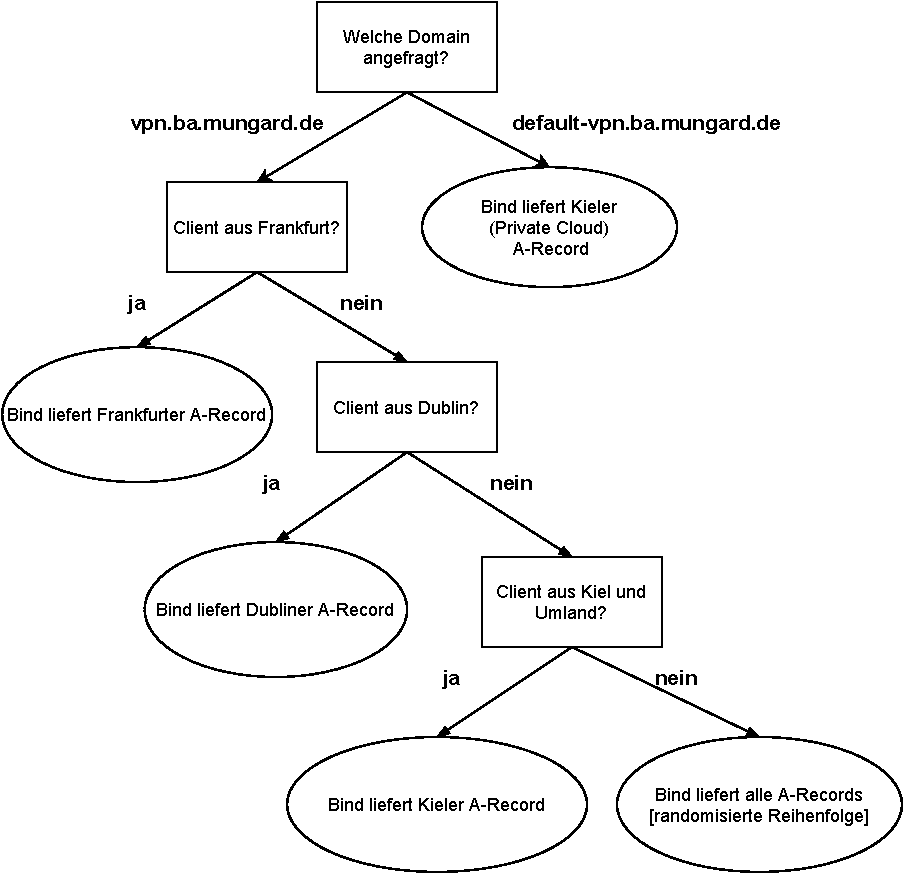
\includegraphics{Figures/entscheidungsbaum_bind_geoip.pdf}
  \caption{Entscheidungsbaum: DNS-Server}
  \label{grafik:Use-Case_2_Entscheidungsbaum_GeoIP}
\end{figure}\FloatBarrier

Fall \ref{server-not-deployed} ist \gls{Client}-seitig gesteuert und kommt dann zum Tragen, wenn der FQDN vpn.ba.mungard.de nicht auflösbar sein sollte (s. Abb. \ref{grafik:Use-Case_2_Entscheidungsbaum_OpenVPN}).

\begin{figure}[h]
  \centering
  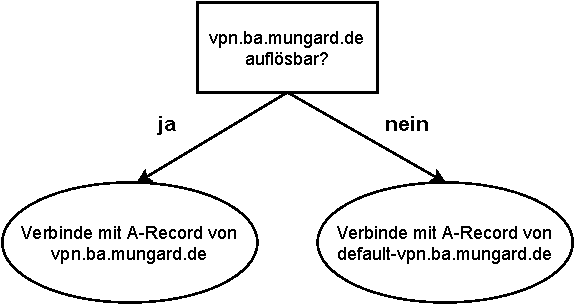
\includegraphics{Figures/entscheidungsbaum_openvpn_config.pdf}
  \caption{Entscheidungsbaum: \gls{Roadwarrior}-VPN}
  \label{grafik:Use-Case_2_Entscheidungsbaum_OpenVPN}
\end{figure}\FloatBarrier

Mit Hilfe des Bind Nameservers ab Version 9.10 ist es möglich, die \gls{GeoIP}-Datenbank des Anbieters MaxMind auszuwerten, um DNS-Anfragen in Abhängigkeit der Absender-IP zu beantworten\cite{bindgeoip2020}. Bei dieser IP handelt es sich typischerweise um die Resolver-IP des \textit{lokalen} Internet-Dienstleisters. Die Annahme für diesen Use-Case ist daher, dass der DNS-Resolver in der gleichen Region wie der \gls{Roadwarrior} angesiedelt ist\label{dns-resolver-region}.\\
Um mit \gls{GeoIP}-Daten der Firma MaxMind arbeiten zu können, muss Bind (Linux-Binary: \texttt{named}) mit einem speziellen Flag (\texttt{-{}-with-maxminddb}) kompiliert werden. Im Ubuntu 20.04 Standardpaket von Bind 9 ist dieses Feature bereits vorhanden (s. Listing \ref{bind-mmdb-compiler-flag}).

%TC:ignore
\begin{listing}[h]
\begin{minted}[breaklines,frame=single]{bash}

$ named -V | grep -o -- '--with-maxminddb'
--with-maxminddb

\end{minted}
\caption{\texttt{named} Compiler-Flags (gefiltert)}
\label{bind-mmdb-compiler-flag}
\end{listing}
%TC:endignore
Der Nameserver muss sowohl extern, also aus dem Internet, als auch intern für verbundene VPN-\gls{Client}s, erreichbar sein. Der Nameserver wird ausschließlich in der Private Cloud gehostet. Es wird von einem \gls{Deployment} eines \textit{secondary} Name-Servers \textit{pro} Standort zur Vereinfachung des \gls{Deployment}s abgesehen. Es sind keine Erkenntnisgewinne dadurch gegeben. Secondary Name-Server halten Kopien aller Zonen des primary Name-Servers vor, welcher für die Verwaltung von Zonendateien zuständig ist \cite[S.517]{Fall2011}.\\
In der Praxis sollte das \gls{Deployment} von \glqq Secondaries\grqq{} aus Redundanzgründen jedoch dringend in Betracht gezogen werden. Außerdem können \glqq verzögerte\grqq{} DNS-Antworten auf Grund sehr großer Entfernungen negative Auswirkungen auf die Usability haben. Da alle Test-Standorte innerhalb von Europa liegen, ist dieser Effekt im Sinne des Proof-of-Concepts vernachlässigbar.\\
Weiterhin müssen Zonen dynamisch editierbar sein, da durch das Terraform-\gls{Deployment} virtuelle Maschinen mit vorher unbekannten IP-Adressen erstellt werden. Diese IP-Adressen müssen mit den Domains der jeweiligen Zonen kombiniert werden. Dies gilt für extern und intern auflösbare Zonen. Für Terraform steht ein Provider \textit{dns} zur Verfügung, der diese dynamischen Updates erlaubt\cite{dnstf2021}.
Das in diesem Kapitel angedeutete Szenario soll wieder per Terraform bereitgestellt werden und setzt direkt auf Use-Case 1 auf. Auf Grund der langen Dauer des \gls{Deployment}s in Use-Case 1 (siehe Kap. \ref{azure-deployment-time}) wird erwogen, Use-Case 2 nicht \glqq komplett\grqq{} auszurollen, sondern Use-Case 1 zu belassen und die Infrastruktur-Komponenten aus Use-Case 2 lediglich hinzuzufügen (vgl. Kap. \ref{accelerate-deployment-use-case-2}).\\
Die OpenVPN-Server sollen auflösbar sein unter der Domain vpn.ba.mungard.de.\\
Als stellvertretender \glqq Applikations-Server\grqq{} soll ein simpler Apache2 pro Standort in einer Ubuntu-VM installiert werden. Dieser soll über die Domain www.intern.ba.mungard.de erreichbar sein.
\subsection{Evaluationskriterien}\label{eval-roadwarrior}
\begin{enumerate}
\item \gls{Roadwarrior}-\gls{Client}s werden simuliert, indem an den entsprechenden Standort (Kiel, Dublin bzw. Frankfurt) eine weitere virtuelle Maschine installiert wird, die VPN-Verbindungen zu den jeweiligen \gls{VPN-Konzentrator}en aufbaut.
\item Ein \gls{Roadwarrior}-\gls{Client} verbindet sich immer mit dem nächstgelegen Standort. Die DNS-Antworten werden per \texttt{dig}- und \texttt{whois}-Kommando verifiziert.
\item Der \gls{Client} hat keine Wahl, mit welchem Standort dieser verbunden wird.
\item Ist ein Cloud-Standort nicht verfügbar (z.B. weil defekt oder nicht bereitgestellt), \textit{muss} der \gls{Client} auf den \textit{default} Standort (Kiel) zurückfallen.
\item Sobald ein \gls{Client} mit einem VPN verbunden ist, muss er die entsprechende interne Server-Ressource ansprechen, die am jeweiligen Standort zur Verfügung steht.
\end{enumerate}

Weitere Evaluationskriterien sind in der Praxis denkbar, spielen im Kontext \textit{Proof-of-Concept}) jedoch keine Rolle.

\chapter{Umsetzung der Use-Cases und Evaluation} \label{Umsetzung der Use-Cases und Evaluation}
Dieses Kapitel beinhaltet die Umsetzung der Use-Cases (\glqq Kerntätigkeiten\grqq{}) und anschließende Evaluation für genannte Kriterien in Kap. \ref{Defintion der Use-Cases} (s. \ref{eval-kriterien-uc1}, \ref{eval-roadwarrior}). Probleme, die in der Umsetzungsphase auftraten, und dazugehörige Lösungsfindung werden gesondert erläutert.

\section{Use-Case 1: Basis Deployment mit Ende-zu-Ende-Konnektivität} \label{Use-Case 1: Basis Deployment}
\subsection{Umsetzung: Kerntätigkeiten}

Im phpIPAM müssen mehrere Netzbereiche reserviert werden. Es werden Netzbereiche benötigt, in denen Maschinen per IPv4 kommunizieren können. Diese Netze werden mit VPC bzw. VNET assoziiert.\\
Für VNET wurde der Netzblock \glqq 10.32.0.0/16\grqq{} und für VPC der Netzblock \glqq 10.33.0.0/16\grqq{} vorreserviert, aus dem kleinere Subnets für die jeweilige Cloud entnommen werden können. Weiterhin ist die Annahme, dass die Private Cloud bereits einen Netzbereich besitzt, in dem Maschinen angesiedelt sind: \glqq 192.168.201.0/24.\grqq{}\\
Es werden \textit{Transfernetzwerke}\label{transfer-azure-aws} benötigt, über die die IPv4-Pakete geschickt werden und die BGP-Präfixe ausgetauscht werden können. AWS sieht hierfür /30-Präfixe aus dem Bereich \glqq 169.254.0.0/16\grqq{} vor \cite{awsvpn2021}, Azure hat eine Range reserviert: \glqq 169.254.21.0\grqq{} -\\ \glqq 169.254.22.255\grqq{} \cite{azurebgp2020}. Als Kompromiss können daher nur Netze aus den Azure-Bereichen genutzt werden, da die Bereiche, die AWS zur Verfügung stellt, größtenteils außerhalb dieser Range liegen. Auch diese Netzbereiche müssen im IPAM vorreserviert werden und für die Transfernetzwerke automatisiert konfiguriert werden.\\
In Listing \ref{apipa-reservation-ipam} wird in phpIPAM nach dem Bereich \glqq TF\_CLOUD\_BGP\_TRANSFER\grqq{}, aus dem alle Transfernetzwerke entommen werden, gesucht. Die Suche passiert per Data Source.\\
Innerhalb des Bereichs wird aus dem vorreservierten Block \glqq Cloud\_Transfer\_BGP\_1\grqq{} ein /30-Netzwerk per resource entnommen. Die Reservierung der Netzblöcke für VPC und VNET erfolgen analog.
%TC:ignore
\begin{listing}[h]
\begin{minted}[breaklines,frame=single]{tf}
//Azure - AWS Transfer
data "phpipam_section" "apipa_main_section" {
  name = "TF_CLOUD_BGP_TRANSFER"
}
data "phpipam_subnet" "apipa_transfer_subnet" {
  section_id = data.phpipam_section.apipa_main_section.section_id
  description_match = "Cloud_Transfer_BGP_1"
} 
resource "phpipam_first_free_subnet" "free_subnet_apipa" {
  parent_subnet_id = data.phpipam_subnet.apipa_transfer_subnet.subnet_id
  subnet_mask = 30
  description = "BGP_AWS_AZURE"
}
\end{minted}
\caption{Reservierung eines /30-Netzwerks in phpIPAM}
\label{apipa-reservation-ipam}
\end{listing}\FloatBarrier
%TC:endignore
Weiterhin werden Pre-Shared-Keys für die Aushandlung der IPsec-Verbindungen benötigt. AWS erzeugt automatisch solche Schlüssel, welche durch die Terraform-Resource \glqq aws\_vpn\_connection\grqq{} zurückgegeben werden. Diese automatisch erzeugten Schlüssel werden daher für die Backbone-Verbindungen AWS $\leftrightarrow$ Azure und AWS $\leftrightarrow$ Private Cloud genutzt. Da Azure diese Schlüssel nicht erzeugt, wurde ein Terraform-Modul geschrieben, welches 24 Zeichen lange Schlüssel erzeugt (s. Lsiting \ref{tf-generate-psk}). Auf Sonderzeichen wird dabei verzichtet. Diese können anschließend genutzt werden für die Backbone-Verbindung Azure $\leftrightarrow$ Private Cloud.
%TC:ignore
\begin{listing}[h]
\begin{minted}[breaklines,frame=single]{tf}
resource "random_password" "random_password" {
  length = 24
  lower = true
  upper = true
  number = true
  special = false
}
output "azure_vyos_tunnel1_psk" {
  value = random_password.random_password.result
  sensitive = true
}
\end{minted}
\caption{Erzeugung eines Pre-Shared-Key in Terraform}
\label{tf-generate-psk}
\end{listing}\FloatBarrier
%TC:endignore
Da, wie bereits erwähnt, für die VyOS-Router keine \textit{native} Terraform-Integration verfügbar ist, wurde zur Konfiguration des Devices eine Vorlage erstellt, welch per CLI Konfigurationen ausrollt.
Die Erzeugung aus der Vorlage erfolgt über die Funktion templatefile()\cite{templatefiletf2021}. Sie erstellt aus einer Template-Datei \underline{vyos\_config.tpl} die Skript-Datei \underline{/tmp/example.sh}. Die Template-Datei wird mit den Variablen \textit{var.aws\_vgw\_ip} und \textit{aws\_tunnel1\_psk} befüllt.
%TC:ignore
\begin{listing}[h]
\begin{minted}[breaklines,frame=single]{tf}
resource "local_file" "vyos_config" {
  filename = /tmp/example.sh
  content = templatefile("${path.module}/include/vyos_config.tpl",
  {
    aws_vgw_ip = var.aws_vgw_ip
    aws_tunnel1_psk = var.aws_tunnel1_psk
  })
}

\end{minted}
\caption{Erzeugung von VyOS-Config-Skript mit templatefile()}
\label{tf-call-tpl-generation}
\end{listing}\FloatBarrier
%TC:endignore
%TC:ignore
Verschiede set-Kommandos werden in Listing \ref{tf-generate-tpl} in das VyOS-Skript eingebettet (Interpreter: \texttt{/bin/vbash}). Die Variablen in Zeilen 9-12 resultieren aus dem Funktionsaufruf (s. Listing \ref{tf-call-tpl-generation}).
\begin{listing}[h]
\begin{minted}[linenos,breaklines,frame=single]{bash}
$ head -n 11 < vyos/include/vyos_config.tpl
#!/bin/vbash
source /opt/vyatta/etc/functions/script-template
configure
#AWS
set vpn ipsec ike-group AWS lifetime '28800'
set vpn ipsec ike-group AWS proposal 1 dh-group '2'
set vpn ipsec ike-group AWS proposal 1 encryption 'aes128'
set vpn ipsec ike-group AWS proposal 1 hash 'sha1'
set vpn ipsec site-to-site peer ${aws_vgw_ip} authentication mode 'pre-shared-secret'
set vpn ipsec site-to-site peer ${aws_vgw_ip} authentication pre-shared-secret ${aws_tunnel1_psk}
set vpn ipsec site-to-site peer ${aws_vgw_ip} description 'VPC tunnel 1'

\end{minted}
\caption{Template für das VyOS-Config-Skript}
\label{tf-generate-tpl}
\end{listing}\FloatBarrier
%TC:endignore
%TC:ignore

Das in \ref{tf-generate-tpl} generierte Shell-Skript wird per \texttt{ssh} auf das Zielsystem (VyOS-Router) kopiert und per Provisioner \textit{remote-exec} ausgeführt.
\begin{listing}[h]
\begin{minted}[breaklines,frame=single]{tf}
resource "null_resource" "vyos_config" {
  connection {
    type = "ssh"
    host = var.vyos_host
    user = var.ssh_user
    private_key = file(var.private_key_file)
  }
  provisioner "file" {
   source = /tmp/example.sh
   destination = var.vyos_script_path
  }
  provisioner "remote-exec" {
    inline = [ "chmod +x ${var.vyos_script_path}", var.vyos_script_path ]
  }
}

\end{minted}
\caption{Kopie per SSH und remote-exec Provisioner}
\label{tf-copy-tpl}
\end{listing}\FloatBarrier
%TC:endignore
\newpage
Folgend werden zentrale Probleme geschildert, die bei der technischen Umsetzung von Use-Case 1 auftraten. Die erarbeiteten Lösungen werden ausführlich erläutert.

\newpage
\subsection{Vertauschung von IPsec-Tunnelparametern}\label{xml-tunnel-parameters}

AWS VPN-Konzentratoren bieten aus Redundanzgründen standardmäßig zwei IPs pro Gegenstelle an. 
%TC:ignore
\begin{listing}[h]
\begin{minted}[breaklines,frame=single]{xml}
<?xml version="1.0" encoding="UTF-8"?>
<vpn_connection id="vpn-096f7fc91dc77cc74">
  [...]
  <ipsec_tunnel>
    <vpn_gateway>
      <tunnel_outside_address>
        <ip_address>18.194.163.131</ip_address>
      </tunnel_outside_address>
      [...]
    </vpn_gateway>
    <ike>
      [...]
      <pre_shared_key>B28VDw7xcqYJZvcWCI7E</pre_shared_key>
    </ike>
    [...]
  </ipsec_tunnel>
  <ipsec_tunnel>
    [...]
    <vpn_gateway>
      <tunnel_outside_address>
        <ip_address>35.157.252.106</ip_address>
      </tunnel_outside_address>
    [...]
    </vpn_gateway>
    <ike>
      [...]
      <pre_shared_key>cHgnL5wZ1vPGTdHhbuLW</pre_shared_key>
    </ike>
    [...]
  </ipsec_tunnel>
</vpn_connection>

\end{minted}
\caption{Die ursprüngliche (gekürzte) XML-Antwort der AWS API}
\label{tf-xml-response-aws}
\end{listing}\FloatBarrier
%TC:endignore
Wie man in Listing \ref{tf-xml-response-aws} sieht, taucht das XML-Element ipsec\_tunnel zwei Mal auf, ist dabei jedoch \textbf{unnummeriert}.
Der Terraform-Provider aws\_vpn\_connection nutzt diese XML-Antwort, um daraus die Rückgabewerte tunnel1\_* und tunnel2\_* zu erzeugen\cite{awsattributestf2021}, die in der weiteren Ausführung von anderen Modulen wiederverwendet werden. Bei einigen Ausführungen wurden diese Elemente Terraform-intern vertauscht: Da nun weder IPsec-Schlüssel noch interne BGP-Peering-Gegenstellen stimmen, kommen weder IPsec-Tunnel noch die BGP-Peering-Sessions hoch. Dieser Bug für den AWS Provider ist in Github seit 2017 dokumentiert\cite{githubbugtf2021}.\\
Mit einem Bash-Skript konnte zumindest ein Workaround gefunden werden, um ein erfolgreiches \gls{Deployment} sicherzustellen. Die Grundannahme ist, dass pro Präfix zwei Pfade auf dem Private Cloud-Router existieren und somit redundant sind (s. Listing \ref{bgp-paths-vyos}). Wenn nur ein Pfad pro Präfix zur Verfügung steht, kam es mit einer hohen Wahrscheinlichkeit zu einer Vertauschung und es muss ein erneutes \gls{Deployment} erfolgen (\texttt{terraform destroy \&\& terraform apply}). Es wird dreimal versucht, eine funktionierende Infrastruktur bereitzustellen, um die APIs der Cloud-Anbieter zu \textit{schonen} und kein Rate-Limiting zu triggern \cite{awsthrottling2021}.
%TC:ignore
\begin{listing}[h]
\begin{minted}[breaklines,frame=single]{bash}
vyos@vyos-cloud:~$ sh ip bgp | grep -A1 -E '10.3[2|3]'
*  10.32.0.0/16     169.254.53.1    100     0   65516 65515 i
*>                  169.254.21.6            0   65515 i
*  10.33.0.0/24     169.254.21.6            0   65515 65516 i
*>                  169.254.53.1    100     0   65516 i

\end{minted}
\caption{Präfixe für AWS und Azure sind redundant sichtbar}
\label{bgp-paths-vyos}
\end{listing}
%TC:endignore
\newpage
Das Beispiel in Abb. \ref{grafik:programmablaufplan_bash_deploy_tf} zeigt den Programmlaufplan des Bash-Skripts \texttt{deploy.sh}. Wenn weniger als zwei Pfade pro Präfix gesehen, findet ein \textit{Re-\gls{Deployment}} statt.

\begin{figure}[h]
  \centering
  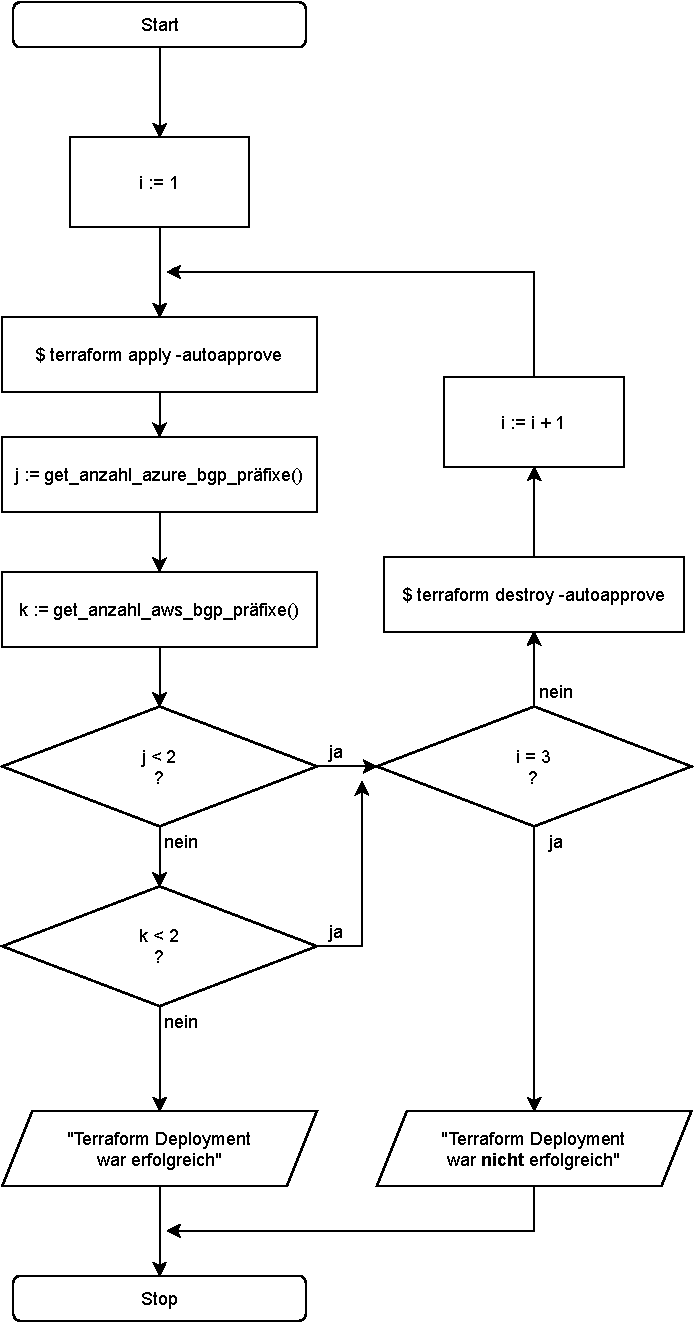
\includegraphics[scale=0.6]{Figures/programmablaufplan_bash_deploy_tf.pdf}
  \caption{Programmablaufplan für das Terraform \gls{Deployment} Skript}
  \label{grafik:programmablaufplan_bash_deploy_tf}
\end{figure}\FloatBarrier
Durch das Bash-Skript konnte die Schwere des Bugs abgemildert werden, um ein funktionierendes Deployment herzustellen. Allerdings führten Re-Deployments zu relativ langen \gls{Deployment}-Zeiten (siehe auch \ref{azure-deployment-time}).\\
Anmerkung: Dieser Bug wurde angeblich noch kurz vor Abgabe dieser Arbeit behoben. Das konnte allerdings nicht mehr verifiziert werden. Es ist im Commit ersichtlich, dass es sich um einen Bug in der internen Sortierfunktion handelt.\cite{awsfixtf2021}
\subsection{Zustandslose VyOS-Konfiguration}
Terraform speichert alle Referenzen auf Infrastrukturkomponenten in der Datei terraform.tfstate (s. Kapitel \ref{tf-provider}). Da es für VyOS keinen vollwertigen Terraform-Provider gibt, wurde mit Templates, die verschiedene \texttt{set}-Kommandos ausführen, gearbeitet.\\
Diese Konfigurationsänderungen sind dadurch völlig zustandlos, da sie nicht invertierbar sind: Terraform kennt nicht die Umkehrung der \texttt{set}-Kommandos, welche benötigt würden, um bei \texttt{terraform destroy} die Konfigurationen am VyOS-Router rückgängig zu machen.

Ein Ansatz wäre gewesen, ein weiteres Template zur Verfügung zu stellen, in dem alle \texttt{set}- durch \texttt{delete}-Kommandos negiert werden.\\
%TC:ignore
\begin{listing}[h]
\begin{minted}[breaklines,frame=single]{bash}
vyos@vyos-cloud# set system time-zone Europe/Berlin
[edit]
vyos@vyos-cloud# delete system time-zone Europe/Berlin
[edit]
\end{minted}
\caption{VyOS: \texttt{delete} negiert das vorherige \texttt{set}-Kommando.}
\label{set-delete-vyos}
\end{listing}\FloatBarrier
%TC:endignore
Per \textit{Destroy-Time Provisioner} würde dieses Template nur bei einem \textit{terraform destroy} genutzt\cite{destroytimeprovtf2021}. Das Problem ist, dass schon bei minimalen Änderungen des Deploy-Templates auch das Destroy-Template angepasst werden muss.
Außerdem sind die IPsec-Konfigurationen relativ umfangreich. Es war zu anzunehmen, dass Relikte aus der Konfiguration übrig bleiben, wenn die Negation aus unbekannten Gründen fehlschlug.
Eine weitere Idee war, mit dem VyOS-Feature \textit{rollback} zu arbeiten. Über eine Commit History werden alle Änderungen an dem System revisionssicher dokumentiert.
%TC:ignore
\begin{listing}[h]
\begin{minted}[breaklines,frame=single]{bash}
vyos@vyos-cloud:~$ show system commit | head -3
0   2021-05-05 09:47:51 by tf via cli
1   2021-05-05 09:25:24 by tf via other
2   2021-05-04 21:17:57 by vyos via cli

\end{minted}
\caption{VyOS Commit History}
\label{commit-history-vyos}
\end{listing}\FloatBarrier
%TC:endignore
So würde man die letzte Revision \textit{vor} der Konfiguration der Backbone-Verbindungen festhalten, um bei einem \texttt{terraform destroy} darauf zurückgehen zu können. Ein Rollback macht einen Neustart erforderlich.
%TC:ignore
\begin{listing}[h]
\begin{minted}[breaklines,frame=single]{bash}
vyos@vyos-cloud# rollback
Possible completions:
  <N>   Rollback to revision N (currently requires reboot)

  Revisions:
    0   2021-05-05 09:47:51 tf by cli
    1   2021-05-05 09:25:24 tf by other
    2   2021-05-04 21:17:57 vyos by cli
    
\end{minted}
\caption{VyOS Rollback auf Revision $N$ nach Neustart}
\label{rollback-cmd-vyos}
\end{listing}\FloatBarrier
%TC:endignore
Es wurden zwei Bash-Skripte geschrieben: \texttt{save\_last\_manual\_commit.sh} speichert die letzte Revision lokal auf dem VyOS-Router, \texttt{apply\_last\_manual\_commit.sh} macht ein Rollback. Terraform speichert per Skript \texttt{save\_last\_manual\_commit.sh} den Zustand vor dem \gls{Deployment} auf dem VyOS-Router (s. Listing \ref{save-last-commit-vyos}).
%TC:ignore
\begin{listing}[h]
\begin{minted}[breaklines,frame=single]{tf}
resource "null_resource" "vyos_config" {
  connection {
    type = "ssh"
    host = var.vyos_host
    user = var.ssh_user
    private_key = file(var.private_key_file)
  }
  [...]
  provisioner "local-exec" {
    command = "${path.module}/bin/save_last_manual_commit.sh"
  }
}

\end{minted}
\caption{Speicherung des letzten Commits vor dem Terraform-Deployment}
\label{save-last-commit-vyos}
\end{listing}\FloatBarrier
%TC:endignore
Nach \textit{terraform apply} liegt auf dem VyOS-Router die Datei \underline{last\_manual\_commit.txt}, die den letzten Zeitstempel vor dem Deployment speichert (s. Listing \ref{save-last-commit-file}).
%TC:ignore
\begin{listing}[h]
\begin{minted}[breaklines,frame=single]{bash}
vyos@vyos-cloud# cat ~tf/last_manual_commit.txt
2021-05-05 09:47:51 by tf via cli
\end{minted}
\caption{Zeitstempel des letzten Commits in Datei \underline{last\_manual\_commit.txt}}
\label{save-last-commit-file}
\end{listing}\FloatBarrier
%TC:endignore
Bei \texttt{terraform destroy} wird das Skript \texttt{apply\_last\_manual\_commit.sh} via Terraform \textit{Destroy-Time Provisioner} ausgeführt, welcher das Rollback mit Hilfe des gespeicherten Zeitstempels auf dem VyOS Router veranlasst (s. Listing \ref{apply-last-commit-vyos}).
%TC:ignore
\begin{listing}[h]
\begin{minted}[breaklines,frame=single]{tf}
resource "null_resource" "vyos_config_destroy" {
  provisioner "local-exec" {
    when = destroy
    command = "${path.module}/bin/apply_last_manual_commit.sh"
  }
}

\end{minted}
\caption{Rollback zur Terraform \glqq Destroy-Time\grqq{}}
\label{apply-last-commit-vyos}
\end{listing}\FloatBarrier
%TC:endignore
\subsection{Lange Laufzeiten für Erstellung von Azure VPN Gateway}\label{azure-deployment-time}
Die Erstellung des Azure VPN Gateways kann bis zu 45 Minuten in Anspruch nehmen\cite{azurevpndeployment2021}. In der Praxis waren es meist etwa 25 Minuten für den Standort \glqq North Europe\grqq{}. Auch das Löschen eines VPN Gateways via \texttt{terraform destroy} dauert bis zu 15 Minuten. Nur wenn dieses Gateway gelöscht wurde, kann ein \textit{Re-\gls{Deployment}} erfolgen, welches vor allem dann notwendig ist, wenn die Vertauschung von IPsec-Parametern (s. Kapitel \ref{xml-tunnel-parameters}) eintrifft.\\
Bei diesem Phänomen handelt es sich nicht um einen Bug im eigentlichen Sinne, macht aber das \gls{Deployment} z.B. für Live-Demonstrationen nicht praktikabel. Da alle weiteren Use-Cases auf diesem Use-Case 1 aufbauen und ebenso in Terraform abgebildet werden sollten, musste eine Lösung gefunden werden, um die \gls{Deployment}-Zeiten zu verkürzen, da jede Änderung des Codes ein (teilweises) Re-\gls{Deployment} notwendig macht (vgl. Kapitel \ref{accelerate-deployment-use-case-2}).
%TC:ignore
\subsection{Evaluation}
Nach dem erfolgreichen \gls{Deployment} wird folgender Status von Terraform zurückgemeldet (s. Listing \ref{tf-base-deployment-ok}).
\begin{listing}[h]
\begin{minted}[breaklines,frame=single]{bash}
Apply complete! Resources: 29 added, 0 changed, 0 destroyed.

Outputs:

aws_subnet_id = "subnet-0192ae38a3a16f584"
[... weitere Output-Variablen ...]
\end{minted}
\caption{Terraform Status nach \gls{Deployment} Use-Case 1}
\label{tf-base-deployment-ok}
\end{listing}\FloatBarrier
%TC:endignore
Die im IPAM reservierten Netze (s. Abb. \ref{grafik:subnet_aws_vpc_reserved}) sind in AWS VPC als Subnets wiederzufinden (s. Abb. \ref{grafik:subnet_aws_vpc_reserved}). Die Prüfung analog für Azure ist ebenso erfolgreich.

\begin{figure}[h]
  \centering
  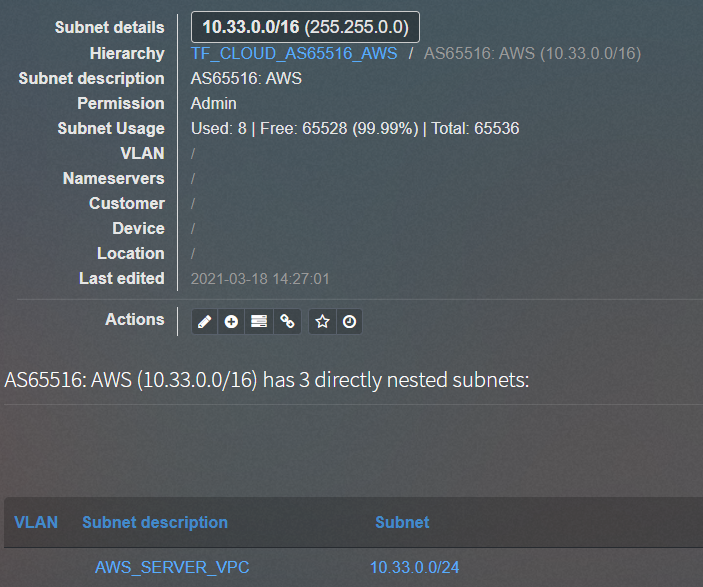
\includegraphics[scale=0.8]{Figures/subnet_aws_ipam_server.png}
  \caption{Reservierung AWS-Subnet in phpIPAM}
  \label{grafik:subnet_aws_vpc_ipam_reserved}
\end{figure}\FloatBarrier

\begin{figure}[h]
  \centering
  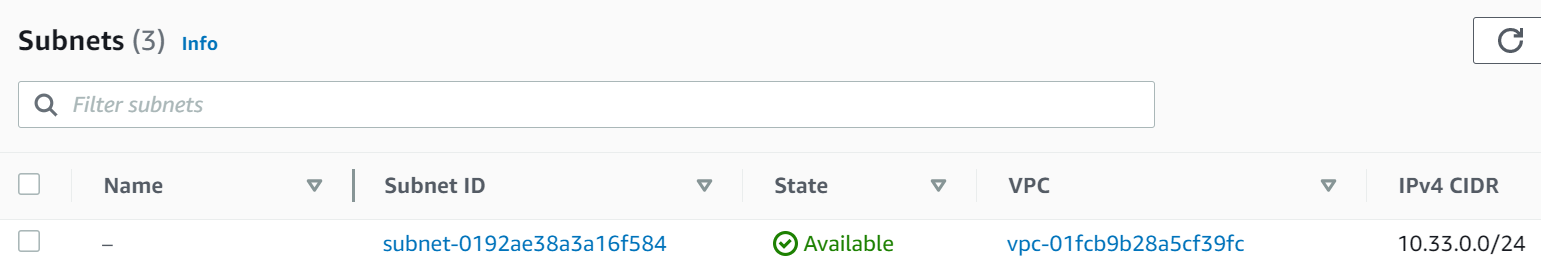
\includegraphics[scale=0.4]{Figures/subnet_aws_reserved_server.png}
  \caption{Das in phpIPAM reservierte Subnet in AWS VPC}
  \label{grafik:subnet_aws_vpc_reserved}
\end{figure}\FloatBarrier
\newpage
Die IPsec Tunnel sind auf dem VyOS-Router konfiguriert und \textit{up} (s. Listing \ref{tf-base-deployment-ipsec-ok}). D.h. Die Tunnel sind aktiv.
%TC:ignore
\begin{listing}[h]
\begin{minted}[breaklines,frame=single]{bash}
vyos@vyos-cloud:~$ show vpn ipsec sa
Connection                     State    Uptime
-----------------------------  -------  --------
[...]
peer-20.67.209.254-tunnel-vti  up       4h43m19s [...]
peer-3.65.181.187-tunnel-vti   up       4h47m26s [...]

\end{minted}
\caption{VyOS IPsec-Tunnel Status}
\label{tf-base-deployment-ipsec-ok}
\end{listing}\FloatBarrier
%TC:endignore
Die Adressen gehören dabei zu Amazon (s. Listing \ref{whois-amazon-public-ip}) bzw. Microsoft.
%TC:ignore
\begin{listing}[h]
\begin{minted}[breaklines,frame=single]{bash}
$ whois 3.65.181.187 | grep -A2 NetRange
NetRange:       3.64.0.0 - 3.79.255.255
CIDR:           3.64.0.0/12
NetName:        AMAZON-FRA

\end{minted}
\caption{Ermittlung der Gegenstelle mit \texttt{whois}}
\label{whois-amazon-public-ip}
\end{listing}\FloatBarrier
%TC:endignore
Außerdem wurden auf dem Cloud-Router die AWS- und Azure-Präfixe via BGP installiert. Pro Präfix sind zwei Pfade vorhanden (s. Listing \ref{bgp-paths-vyos}).

Es wurde pro Cloud eine virtuelle Maschine (Ubuntu) installiert, um die Ende-zu-Ende-Konnektivität zu prüfen. Der Ping in Listing \ref{tf-base-deployment-ping-ok} von VM in AWS VPC $\rightarrow$ VM Azure VNET ist erfolgreich. Analog waren alle weiteren Ping-Tests zwischen den Cloud-Plattformen erfolgreich.
%TC:ignore
\begin{listing}[h]
\begin{minted}[breaklines,frame=single]{bash}
ubuntu@ip-10-33-0-121:~$ ping -c1 10.32.0.4
PING 10.32.0.4 (10.32.0.4) 56(84) bytes of data.
64 bytes from 10.32.0.4: icmp_seq=1 ttl=63 time=25.7 ms

--- 10.32.0.4 ping statistics ---
1 packets transmitted, 1 received, 0% packet loss, time 0ms
rtt min/avg/max/mdev = 25.729/25.729/25.729/0.000 ms
\end{minted}
\caption{Ping-Tests zwischen verschiedenen Cloud-Plattformen}
\label{tf-base-deployment-ping-ok}
\end{listing}\FloatBarrier
%TC:endignore
Es wurden vereinzelte Messungen in verschiedene Richtungen mit dem Werkzeug \texttt{iperf3} gemacht, welches Bandbreitenmessungen ermöglicht. Es zeigt grundsätzlich \glqq ordentliche\grqq{} Bandbreiten (s. Listing \ref{iperf3-vpc-vnet}).

%TC:ignore
\begin{listing}[h]
\begin{minted}[linenos,breaklines,frame=single]{bash}
root@vyos-aws-ovpn-gw:~# iperf3 -c 10.32.0.5
Connecting to host 10.32.0.5, port 5201
[  4] local 10.33.2.93 port 44298 connected to 10.32.0.5 port 5201
[ ID] Interval           Transfer     Bandwidth       Retr  Cwnd
[  4]   0.00-1.00   sec  32.8 MBytes   275 Mbits/sec   45   1.52 MBytes
[  4]   1.00-2.00   sec  41.2 MBytes   346 Mbits/sec    0   1.66 MBytes
[  4]   2.00-3.00   sec  40.0 MBytes   336 Mbits/sec    0   1.78 MBytes
[  4]   3.00-4.00   sec  37.5 MBytes   315 Mbits/sec   17   1.33 MBytes
[  4]   4.00-5.00   sec  33.8 MBytes   283 Mbits/sec    0   1.40 MBytes
[  4]   5.00-6.00   sec  41.2 MBytes   346 Mbits/sec    0   1.45 MBytes
[  4]   6.00-7.00   sec  41.2 MBytes   346 Mbits/sec    0   1.49 MBytes
[  4]   7.00-8.00   sec  43.8 MBytes   367 Mbits/sec    0   1.51 MBytes
[  4]   8.00-9.00   sec  42.5 MBytes   357 Mbits/sec    0   1.52 MBytes
[  4]   9.00-10.00  sec  41.2 MBytes   346 Mbits/sec    0   1.53 MBytes
- - - - - - - - - - - - - - - - - - - - - - - - -
[ ID] Interval           Transfer     Bandwidth       Retr
[  4]   0.00-10.00  sec   395 MBytes   332 Mbits/sec   62             sender
[  4]   0.00-10.00  sec   394 MBytes   330 Mbits/sec                  receiver
\end{minted}
\caption{Bandbreitenmessung AWS VPC $\rightarrow$ Azure VNET}
\label{iperf3-vpc-vnet}
\end{listing}\FloatBarrier
%TC:endignore
Man sieht allerdings an Zeile 18, dass TCP Retransmissions (\glqq Retr 62\grqq{}) stattgefunden haben. Es ist wahrscheinlich, dass ein \textit{Flaschenhals} existiert, Paketverluste konnten mit diversen Ping-Messungen (s. Listing \ref{tf-base-deployment-ping-ok}) nicht festgestellt werden.\\
Es werden Bandbreiten, insofern sich nicht ein deutlicher negative Auswirkungen wahrgenommen werden, in dieser Arbeit nicht tiefergehend untersucht (s. Kapitel \ref{abgrenzung}). Ein Ausblick zu Bandbreitenoptimierung wird im Ausblick gegeben (s. Kapitel \ref{ausblick}). Es wurde an dieser Stelle mit einem Floodping lediglich untersucht, ob sich ein deutlicher Paketverlust bemerkbar macht (s. Listing \ref{floodping}).
%TC:ignore
\begin{listing}[h]
\begin{minted}[breaklines,frame=single]{bash}
root@vyos-azure-ovpn-gw:~# /bin/ping -s 1200 -c 1000 -f 10.33.2.93
PING 10.33.2.93 (10.33.2.93) 1200(1228) bytes of data.

--- 10.33.2.93 ping statistics ---
1000 packets transmitted, 1000 received, 0% packet loss, time 13370ms
rtt min/avg/max/mdev = 25.968/28.533/173.755/10.763 ms, pipe 11, ipg/ewma 13.384/27.159 ms
\end{minted}
\caption{Floodping Azure $\rightarrow$ AWS}
\label{floodping}
\end{listing}\FloatBarrier
%TC:endignore

Um die Redundanz zu des Backbones zu testen, wurden von allen Teilnehmern zu allen Teilnehmern Ping-Tests gemacht und währenddessen eine Verbindung getrennt. Da ein Präfix über zwei Pfade zu sehen ist, ist die Erwartung, dass ein Backup-Pfad genutzt wird (s. Listing \ref{grafik:Use-Case-1_Basis_Deployment_missing_link}).\\

\begin{figure}[h]
  \centering
  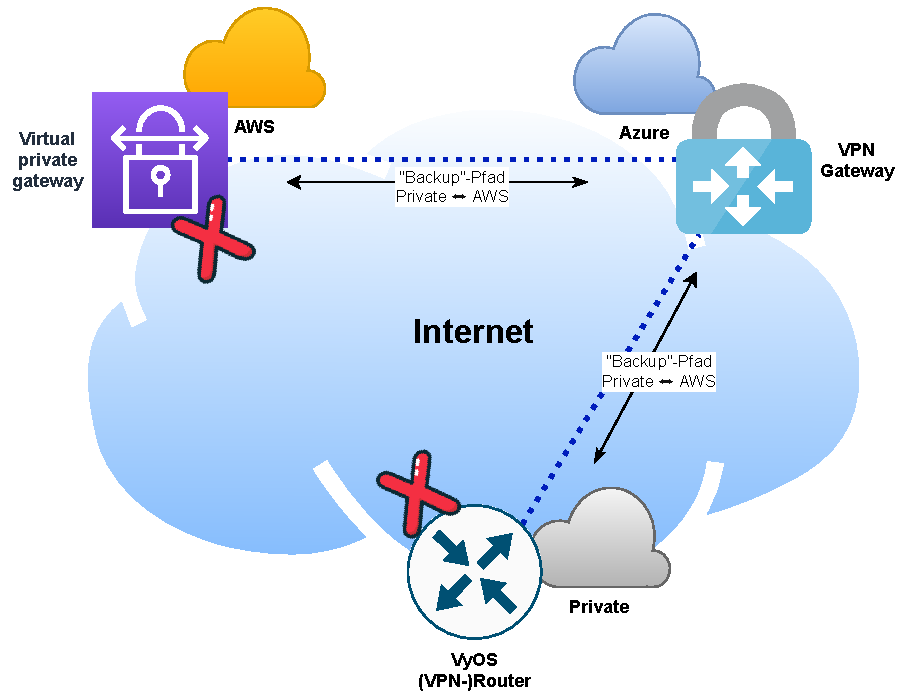
\includegraphics{Figures/Use-Case-1_Basis_Deployment_missing_link.pdf}
  \caption{Backbone mit einer fehlenden Verbindung zwischen Private Cloud und AWS}
  \label{grafik:Use-Case-1_Basis_Deployment_missing_link}
\end{figure}\FloatBarrier

Man kann in Listing \ref{tf-base-deployment-ping-ok-missing-link} sehr gut erkennen, dass das BGP eine Konvergenzzeit erfordert, bis die Pakete über einen anderen Pfad laufen. \textit{ping} versendet in der Standardkonfiguration im Interval von einer Sekunde ICMP-Echo-Request-Pakete. Daraus lässt sich schlussfolgern, dass die Verbindung in Listing \ref{tf-base-deployment-ping-ok-missing-link} etwa 44 Sekunden unterbrochen war.\\
Weiterhin hat sich die Round-Trip-Time von ~20 ms auf ~62 ms erhöht. Dies ist eine logische Konsequenz, da Pakete nun längere Wege (\textit{mehr Hops}) zurücklegen müssen. Alle Ping-Tests waren trotz Kappen einer Verbindung erfolgreich. Man muss dabei allerdings Paketverluste während der Konvergenzzeit hinnehmen.
%TC:ignore
\begin{listing}[h]
\begin{minted}[breaklines,frame=single]{bash}
root@www:~# ping 10.33.0.121
PING 10.33.0.121 (10.33.0.121) 56(84) bytes of data.
[...]
64 bytes from 10.33.0.121: icmp_seq=15 ttl=61 time=19.9 ms
64 bytes from 10.33.0.121: icmp_seq=16 ttl=61 time=24.3 ms
64 bytes from 10.33.0.121: icmp_seq=17 ttl=61 time=19.6 ms
64 bytes from 10.33.0.121: icmp_seq=18 ttl=61 time=19.7 ms 
--- Kappen einer Verbindung nach ICMP Sequenznummer 18 ---
--- Recovery zu ICMP Sequenznummer 62 via Backup-Pfad ----
64 bytes from 10.33.0.121: icmp_seq=62 ttl=61 time=67.4 ms
64 bytes from 10.33.0.121: icmp_seq=63 ttl=61 time=62.2 ms
64 bytes from 10.33.0.121: icmp_seq=64 ttl=61 time=62.5 ms
64 bytes from 10.33.0.121: icmp_seq=65 ttl=61 time=62.4 ms
[...]
\end{minted}
\caption{Ping-Tests zwischen den Cloud-Plattformen mit Kappen einer Backbone-Verbindung}
\label{tf-base-deployment-ping-ok-missing-link}
\end{listing}\FloatBarrier
%TC:endignore
Alle Evaluationskriterien (siehe Kapitel \ref{eval-kriterien-uc1}) wurden somit erfüllt und der Use-Case konnte erfolgreich umgesetzt werden.

\section{Use-Case 2: Road Warrior} \label{Use-Case 2: Road Warrior}
%Anforderung: Ende-zu-Ende-Erreichbarkeit! Für z.B. Endpoint Scanning
%Gleiches Profil für alle VPN-Konzentratoren

\subsection{Umsetzung: Kerntätigkeiten}

%GeoIP
%Terraform DNS Update
%Bind Split-DNS

In AWS und Azure wurden via Terraform die virtuellen Maschinen VyOS aus den jeweiligen Marketplaces installiert.
Es wurden für die Cloud-Standorte AWS und Azure analog zu Use-Case 1 Templates erstellt, um den Client-VPN-Konzentrator zu installieren. In der Terraform Ressource azurerm\_linux\_virtual\_machine wird das richtige VyOS-Image aus dem Cloud-Marketplace referenziert über source\_image\_reference und lässt dieses installieren. Einige dieser Markeplace-Images bieten verschiedene Support- und Lizenz-Verträge an. Über den \textit{plan \{\}}-Kontext wird der passende Contract ausgewählt (hier: \glqq Standard support\grqq{}). Ähnlich ist für die AWS-Instanz vorzugehen.

\begin{lstlisting}[label=tf-azure-vyos-machine-image,caption=Mit der Terraform-Ressource wird das passende VyOS-Image gesucht und installiert.]
resource "azurerm_linux_virtual_machine"  "azurerm_linux_virtual_machine" {
  name = "vyos-test"
  location = var.rg_location
  resource_group_name = var.rg_name
  admin_username = "vyos"
  size = "Standard_B1s"
  network_interface_ids = [ azurerm_network_interface.azurerm_network_interface.id ]
  os_disk {
    caching = "ReadWrite"
    storage_account_type = "Premium_LRS"
  }
  admin_ssh_key {
    username   = "vyos"
    public_key = file("~/terraform/.cred_mgmt/_push/authorized_keys/id_rsa_automation.pub")
  }
  source_image_reference {
    publisher = "sentriumsl"
    offer = "vyos-1-2-lts-on-azure"
    version = "latest"
    sku = "vyos-1-2-crux"
  }
  plan {
    name = "vyos-1-2-crux"
    product = "vyos-1-2-lts-on-azure"
    publisher = "sentriumsl"
  }
}
\end{lstlisting}

Konfiguriert wurden die virtuellen Maschinen wieder über ein Terraform-Template. Das Public/Private-Schlüsselpaar wurde vorab erstellt, von der pfSense-PKI signiert und mit dem Zertifikat auf dem Terraform-Server gespeichert. Während des Terraform-Deployments wird Private Key und Zertifikat per Terraform Provisioner auf das Zielsystem kopiert. Sie werden in der Config dann via set interfaces openvpn vtun0 tls cert-file / key-file referenziert. In der Praxis sollte darauf verzichtet werden, das Schlüsselmaterial \glqq auf einem anderen System vorzulagern \grqq{}: ein privater Schlüssel nur auf dem Server erzeugt und gespeichert werden, auf dem dieser final genutzt wird. Optimalerweise wäre dies zur Laufzeit der Terraform-Deployments. Zur Vereinfachung des Use-Cases wurde auf diesen Schritt verzichtet. Eine Möglichkeit zur automatisierten Erzeugung von vertrauenswürdigen Zertifikaten ist das Simple Certificate Enrollment Protocol (SCEP)\cite[S.554]{Schmeh2013}.

Für den sich verbindenden VPN-Client sind diverse Konfigurationen hinterlegt: Domain-Name, (interner) Name-Server und Routen, die über den VPN-Konzentrator erreicht werden können.
Weiterhin wird ein MSS-Clamping vorgenommen, um IP-Fragmentierung von TCP-Applikationen möglichst zu verhindern.\\
Das Subnetz, in dem die OpenVPN-Clients terminiert werden, wird wieder dynamisch aus dem IPAM alloziert (s. set interfaces openvpn vtun0 server subnet).

\begin{lstlisting}[label=vpn-c2s-server-config,caption=Terraform Template für VyOS OpenVPN-Server in AWS]
set interfaces openvpn vtun0 openvpn-option "--mssfix 1350"
set interfaces openvpn vtun0 server domain-name 'intern.ba.mungard.de'
set interfaces openvpn vtun0 server name-server '192.168.201.1'
#"dynamic" routes?
set interfaces openvpn vtun0 server push-route '10.32.0.0/16'
set interfaces openvpn vtun0 server push-route '10.33.0.0/16'
set interfaces openvpn vtun0 server push-route '192.168.201.0/24'
set interfaces openvpn vtun0 server subnet ${aws_vpn_clients_subnet}/${aws_vpn_clients_subnet_mask}
set interfaces openvpn vtun0 tls ca-cert-file '/config/auth/BA_CA_2021.crt'
set interfaces openvpn vtun0 tls cert-file '/config/auth/vpn-server-aws.ba.mungard.de.crt'
set interfaces openvpn vtun0 tls dh-file '/config/auth/dh2048.pem'
set interfaces openvpn vtun0 tls key-file '/config/auth/vpn-server-aws.ba.mungard.de.key'
\end{lstlisting}

Die drei Cloud-Standorte wurden in diesem Proof-of-Concept verteilt über verschiedenen Regionen: Dublin (Azure), Frankfurt (AWS), Kiel (Private Cloud). Es werden drei Roadwarrior-Clients simuliert, die ebenso am jeweiligen Standort stehen. Dazu wurden weitere VMs an den Cloud-Standorten hochgefahren: Sie wurden völlig isoliert von dem restlichen Deployment installiert und sich nicht Teil der internen Infrastruktur. Zugang zu internen Ressourcen wird nur über eine erfolgreiche Authentifizierung am VPN-Konzentrator gewährleistet.

\begin{lstlisting}[label=ext-ip-addr-roadwarrior,caption=Der simulierte Roadwarrior-Client ist nicht Teil der Netzwerke 10.32.0.0/16 bzw. 10.33.0.0/16]
ubuntu@vpn-client-azure:~$ ip -brief -4 address show | grep -v lo
eth0             UP             10.42.0.4/24
\end{lstlisting}

Internet-Traffic ist möglich, Zugriff auf interne Ressourcen ist nicht möglich: 192.168.201.1 ist eine IP-Adresse der Private Cloud.

\begin{lstlisting}[label=internet-access-roadwarrior,caption=Der Roadwarrior-Client kann auf das Internet zugreifen, jedoch nicht auf interne Ressourcen ohne VPN-Einwahl]
#Internet-Traffic
ubuntu@vpn-client-azure:~$ ping -c 1 8.8.8.8
PING 8.8.8.8 (8.8.8.8) 56(84) bytes of data.
64 bytes from 8.8.8.8: icmp_seq=1 ttl=112 time=0.987 ms

--- 8.8.8.8 ping statistics ---
1 packets transmitted, 1 received, 0% packet loss, time 0ms
rtt min/avg/max/mdev = 0.987/0.987/0.987/0.000 ms

#Interne Adresse ist nicht erreichbar 
ubuntu@vpn-client-azure:~$ ping -c 1 192.168.201.1
PING 192.168.201.1 (192.168.201.1) 56(84) bytes of data.

--- 192.168.201.1 ping statistics ---
1 packets transmitted, 0 received, 100% packet loss, time 0ms
\end{lstlisting}

Die MaxMind GeoIP-Datenbank wurde auf dem DNS-Server installiert und in der Bind-Konfiguration referenziert:

\begin{lstlisting}[label=bind-geoip-directory,caption=.]
$ grep -E 'options|geoip-directory|^};' < named.conf.options
options {
        geoip-directory "/usr/share/GeoIP";
};
\end{lstlisting}

Dadurch wurde ermöglicht, GeoIP-Daten in einer Access Control List (ACL) zu nutzen und verschiedene Fälle zu definieren. Die ACL heißt in diesem Falle \glqq dublin\grqq{} und erlaubt Zugriffe aus der Stadt Dublin bzw. Zugriff für den TSIG-Key db-vpn.ba.mungard.de. Dieser Key wird benötigt, um Zonen-Updates machen zu können und ist im entsprechenden Terraform-Modul hinterlegt.

\begin{lstlisting}[label=acl-geoip-bind,caption=.]
acl "dublin" {
        geoip city Dublin;
        key "db-vpn.ba.mungard.de.";
};
\end{lstlisting}

Weiterhin existiert ein \textit{View} \glqq Dublin\grqq{}, in dem die ACL und Zonen-Daten zusammengeführt werden. Mit \textit{allow-update} werden Zonen-Updates explizit und ausschließlich für genannten TSIG-Key erlaubt.

\begin{lstlisting}[label=view-geoip-bind,caption=.]
view "dublin" {
        match-clients { dublin; };
        zone "ba.mungard.de" {
                type master;
                file "/etc/bind/ba_zones/db.geo.ba.mungard.de-dublin";
                allow-update { key "db-vpn.ba.mungard.de."; };
        };
};
\end{lstlisting}

In der Zonen-Datei für Dublin befindet sich vor Terraform-Deployment nur ein A-Record \textit{default-vpn}. Dies ist der A-Record, der als Fallback dient. Gemäß Evaluationskriterien muss ein Roadwarrior-Client auf die Private Cloud zurückfallen, wenn bisher kein Deployment stattgefunden hat. Die öffentlich auflösbare Zone lautet \textit{ba.mungard.de}.

\begin{lstlisting}[label=zone-dublin-before-deployment,caption=Die Zone ba.mungard.de vor dem Terraform-Deployment.]
$ grep -A1 "ORIGIN ba.mungard.de" < /etc/bind/ba_zones/db.geo.ba.mungard.de-dublin
$ORIGIN ba.mungard.de.
default-vpn             A       195.244.254.197
\end{lstlisting}

Die Konfigurationen für Frankfurter und Kieler Clients wurden analog vollzogen.

Analoges Vorgehen mit Split-View-DNS intern, nur kein GeoIP

Binärer Entscheidungsbaum Bind / OpenVPN

match-all wenn weder Frankfurt, Dublin oder Kiel...





%OpenVPN Client Config

\subsection{Probleme und Lösungsfindung}
%VyOS Images finden? az CLI, AWS Suche funktioniert nicht
%Lizenzen muss zugestimmt werden -> manuell!!!!
%Statische Routen innerhalb VPC nicht more specific -> Transit Gateway
%Import von Remote State, um Azure VPN Gateway zu verkürzen... Eigentlich ziemlich coole Idee von mir... :)
%Die richtigen Images für die VyOS-Maschinen der jeweiligen Cloud-Marketplaces auf Terraform zu übertragen, erwies sich als nicht trivial...
%mmdb.py damit man nicht "blind" ist...
\subsection{Evaluation}
%dig für "next hop"
\chapter{Schlussbetrachtung} \label{Fazit und Ausblick}
%Anforderung: Ende-zu-Ende-Erreichbarkeit! Für z.B. Endpoint Scanning
%Gleiches Profil für alle VPN-Konzentratoren

\section{Fazit}

In dieser Arbeit konnte erfolgreich demonstriert werden, dass eine sichere und isolierte Hybrid Cloud-Vernetzung ohne den Einsatz von proprietären Herstellerlösungen möglich ist. Robuste und offen dokumentierte Technologien wie IPsec, DNS oder BGP, welche im Internet schon seit Jahrzehnten genutzt werden, haben auch in \glqq modernen\grqq{} Cloud-Umgebungen weiterhin ihre Berechtigung.\\
Im Allgemeinen konnten die Vorerfahrungen des Autors aus dem \textit{klassischen} Netzwerkbereich gewinnbringend genutzt werden, um sie auf Ideen und Technologien des (hybriden) Cloud-Networkings zu übertragen: Am Ende des Tages werden auch in dieser Disziplin Pakete von A nach B verschickt et vice versa. Cloud-Ingenieure der \textit{Big Player} AWS und Azure werden nicht bei jeder erdenklichen Möglichkeit das Rad neu erfinden.\\
Es reicht aber auch nicht, sich ausschließlich auf das vorhandene Skill-Set zu berufen. Es haben eben nicht mehr alle Paradigmen aus der \glqq alten Welt\grqq{} ihre Gültigkeit: Technologien kamen dazu, zum Teil wurden alte Zöpfe abgeschnitten. So sind OSI-Layer 1 und 2 für den Netzwerk-Administrator in der Cloud gewissermaßen nicht existent und spielen keine Rolle mehr. Im Gegenzug muss dieser sich jedoch mit neuen Werkzeugen beschäftigen. Das hier genutzte Automatisierungswerkzeug Terraform ist nur eines unter vielen.\\
%Silos wie sie auch bei NetUSE der Fall sind...
Silodenken, bei dem Netzwerk, Security, Datenbanken, etc. in Einzeldisziplinen aufgeteilt werden, ist nicht mehr zeitgemäß, da diese Komponenten im Cloud-Umfeld noch viel enger vermascht sind. Auch die Entkoppelung von der \glqq wahren\grqq{}, physischen Infrastruktur und die dadurch unterstützte Annahme, dass durch eine \glqq Cloud-Magie\grqq{} alles problemlos und für alle Ewigkeiten funktioniert, kann sich dabei als zu fahrlässig herausstellen. So kann (und will) man gar nicht mehr wissen, \glqq welches Bit über welchen Draht im Rechenzentrum läuft\grqq{}, aber eine gute technische Ressourcenplanung und das Durchdenken von Fail-Over-Szenarien sind nach wie vor unentbehrliche Prozesse. Dies hat der Brand im Straßburger Rechenzentrum des Cloud-Providers OVH nochmals deutlich vor Augen geführt\cite{ChristofKerkmann2021}.\\
So konnte mit Use-Case 1 demonstriert werden, wie ein verteilter Internetdienst über Cloud-Grenzen hinweg existieren und dadurch redundant ausgelegt werden kann. Ein Re-Routing von Paketen erfolgt, falls eine Verbindung zwischen Cloud-Standorten wegfällt. Es lassen sich dabei noch weitere VPN-Verbindungen zu Gegenstellen bereitstellen, um die Redundanz und Bandbreite nochmals zu erhöhen (siehe \ref{ausblick}).\\
In Use-Case 2 konnte erfolgreich gezeigt werden, wie geobasiertes DNS genutzt werden kann, um Verbindungen mit niedrigen Latenzen zu gewährleisten. Weiterhin ist es möglich, Infrastruktur neu zu provisionieren und daraufhin direkt per DNS erreichbar zu machen.\\ 
Die in der Arbeit aufgezeigten Use-Cases können mit Hilfe von Terraform und IPAM automatisiert ausgerollt und wieder zurückgebaut werden. In der Praxis, bei der bei Kunden keine \glqq grüne Wiese\grqq{} vorherrscht, kann u.U. nicht auf dieses Tooling zurückgegriffen und es muss im Einzelfall betrachtet werden, welche Schnittstellen und Werkzeuge bereits genutzt werden bzw. sinnvoll erscheinen. Grundlegend lässt sich sagen, dass sich viele Themen mit Fokus Cloud in irgendeiner Form automatisieren lassen. Public Clouds sind grob umschrieben große \glqq Baukasten-Systeme\grqq{} mit diversen Kombinationsmöglichkeiten.\\
Dabei spielt das eigentliche Tooling nur eine untergeordnete Rolle: wichtig ist im Sinne des Kunden eine Kostensenkung durch fehlerarme und optimierte Prozesse. Bevor Prozesse aber automatisiert abgebildet werden können, bedürfen sie einer genauen Erfassung mit gleichzeitiger Formulierung von messbaren (Kosten-)Kriterien.% Ein kompletter Umstieg auf Cloud-Computing inkl. Automatisierungs-Layer bedeutet dabei nicht pauschal die \glqq beste\grqq{} Lösung.\\

Sollte eine Hybrid Cloud-Strategie in Erwägung gezogen werden, muss man sich bewusst sein, dass man technologisch oftmals mit dem \textit{kleinsten gemeinsamen Vielfachen (kgV)} arbeitet. Dieses Projekt war insofern eine dankbare Aufgabe, als die Public Cloud-Provider AWS und Azure offene Technologien für VPN und Routing anbieten. Würde jedoch nur eine Plattform bspw. keine BGP-Unterstützung haben, hätte sich das kgV verändert: Änderungen der Topologie oder ein kompletter Verzicht auf dynamisches Routing hätten in Betracht gezogen werden müssen. Kleinere aber lösbare Probleme offenbarten sich bereits bei der Auswahl des richtigen Transfernetzes für das BGP-Peering (siehe \ref{transfer-azure-aws}) oder der Auswahl des VPN-Konzentrators für Roadwarrior-VPN (siehe \ref{uc1-vorauswahl}).\\
Hersteller von SD-WAN Lösungen versuchen diese Probleme zu umgehen, indem mehr oder weniger \textbf{alle} Netzwerk-Logiken in virtuelle Maschinen ausgelagert werden. Nachteile wurden mit Vendor Lock-In und somit fehlender Interoperabilität bereits genannt. Weiterhin ist dabei die Annahme, dass alles so bleibt wie zum Zeitpunkt des \gls{Deployment}s. Jedoch ist Cloud technologisch ein \textit{moving target}: APIs oder notwendige Technologien können sich jederzeit ändern oder abgekündigt werden\cite{Yegge2020}. Gehen Hersteller dann schnellstmöglich auf Änderungen bei den Cloud-Providern ein? Können Bugfixes dann problemlos eingespielt werden, ohne die Produktion zu gefährden?\\ 
Die Gefahr, dadurch einen Single-Point-Of-Failure ins Netzwerk zu integrieren, ist hoch, wenn man bedenkt, dass vergleichbare Lösungen meist ohne den Einsatz von \glqq Proxies\grqq{} erreicht werden können und direkt von den Cloud-Providern unterstützt werden.


%Industriedruck...
%
%Die Hoffnung ist, dass die Standards von AWS und Azure direkt supportet werden...
%AWS Azure machen Änderungen wenn unten drunter... SPOF?
%Außerdem beschäftigt man sich nicht mit Cloud...



%Das hätte auch für das interne Routing sicherlich Konsequenzen gehabt... (das was am Ende auch SD-WAN Anbieter machen...) aber auch hier (s. Transfernetzwerk...) Dies kann je nach Definition des Scopes unterschiedliche Auswirkungen haben.
%
%Spezielle Building Blocks... nicht erreichbar für andere Teilnehmer, nicht vorhanden in anderen Clouds...
%
%dass alle Buildings Blocks, die genutzt werden, möglichst generisch nutzbar sein müssen. Spezielle

%MPLS LINK
%2. Satz in Einleitung
%https://steve-yegge.medium.com/dear-google-cloud-your-deprecation-policy-is-killing-you-ee7525dc05dc
%Bei SD-WAN geht es z.B. darum, verschiedene (Cloud-)Standorte miteinander zu vernetzen, ohne auf teure Anschlüsse wie MPLS angewiesen zu sein. Durch geeignete Abstraktionsschichten soll ähnlich wie in der Arbeit eine Ende-zu-Ende-Konnektivität über Standorte ermöglicht werden. 
%https://aws.amazon.com/marketplace/search?searchTerms=sd-wan
%Viele Hersteller haben die Zeichen der Zeit erkannt und versprechen, den Umstieg auf Cloud zu erleichtern und warten mit einem großen Produktportfolio auf. Eine Gefahr, neben dem bereits angesprochenen Vendor Lock-In, besteht für den Kunden allerdings bei solchen Lösungen darin, dass Cloud-Computing stetig im Wandel ist - im Gegensatz zum klassischen Betrieb eines Rechenzentrums. APIs oder Technologien können abgekündigt werden. Gehen die Hersteller dann schnellstmöglich auf Änderungen ein? Können neue Features und Bugfixes dann eingespielt werden, ohne die Produktion zu gefährden? Wohlgemerkt kann eine Abkündigung ebenso Tools wie Terraform treffen. Optimalerweise ohne Änderungen am Code zu machen.   
%Alter Wein aus neuen Schläuchen

%Wohlgemerkt kann dies auch die hier vorgestellten Automatisierungstools treffen, Terraform hat eine große, wachsende Community. Bei Problemen ist man alleine auf den Hersteller angewiesen
%ist der falsche Ansatz / Portierung von alt nach neu kann auch gefährlich sein... das holt einen ein... Freischaltungen??
%vielleicht wirds vorher schon in Terraform gefixt
%z.B (s. ...) (Workarounds mit TG, Route Table, Next Hop Routing...). Kleinster gemeinsamer Nenner...

\section{Ausblick}\label{ausblick}
%EDNS Client Subnet https://datatracker.ietf.org/doc/html/rfc7871
Wie bereits in der Abgrenzung geschrieben, sollte in dieser Arbeit wenig auf (mögliche) Bandbreiten eingegangen werden, da diese von zu vielen Faktoren beeinflusst werden kann:
\begin{itemize}
    \item Sind die virtuellen Maschinen und VPN Building Blocks performant genug, um die verfügbaren Bandbreiten auszunutzen?
    \item Sind die Verschlüsselungsparameter der Tunnel optimal gewählt?
    \item Unterscheiden sich Bandbreiten zwischen verschiedenen Protokollen (UDP \textit{versus} TCP bspw.) eklatant?
    \item Ermöglichen Cloud-Plattformen Optimierungen wie z.B. TCP-Offloading?
    \item Wird auf einer Verbindung fragmentiert? Wie wirken sich verschiedene MTU-Parameter aus?
    \item Sind die Cloud-Standorte (Dublin und Frankfurt) Routing-technisch \textit{zu weit} voneinander entfernt?
    %https://aws.amazon.com/premiumsupport/knowledge-center/transit-gateway-ecmp-multiple-tunnels/
    %https://docs.microsoft.com/en-us/azure/vpn-gateway/vpn-gateway-highlyavailable
    \item Wie kann sich Equal Cost Multipath (ECMP) auf die verfügbare Bandbreite auswirken? Funktioniert ECMP richtungsunabhängig?
\end{itemize}
Grundsätzlich hat sich im Laufe dieser Arbeit gezeigt, dass die Verbindungen, auch durch die zusätzliche Redundanz des Backbones, stabil sind. Weiterhin war \textit{subjektiv} die Performance gut, wenn zum Beispiel über den Tunnel auf entfernten Systemen gearbeitet wurde per SSH. Wie vereinzelte Messungen (siehe \ref{iperf3-vpc-vnet}) zeigen, existiert wahrscheinlich zwischen AWS und Azure ein Flaschenhals. Hohe Paketverluste, die dies rechtfertigen würden, sind nicht zu messen.
Um genauere Aussagen diesbezüglich treffen zu können, wäre eine weitere Ausarbeitung in Form einer Bachelor-/Master-Arbeit vorstellbar. Dort könnte z.B. nach Definition von Performance-Kriterien typischer Anwendungen untersucht werden, wie sich Variationen in oben genannten Punkten auf Bandbreiten auswirken. Jitter, Latenz und Paketverlust wären weitere Parameter, die man untersuchen könnte. Als Basiswert könnten Service-Level-Agreements von AWS und Azure herangezogen werden.\\
Es könnte ein geeignetes Tooling entwickelt werden, um Standorte dauerhaft zu messen und ggf. temporär aus einer Topologie herauszunehmen, sollten Kriterien nicht mehr erfüllbar sein. Durch geeignete Automatisierungsmechanismen müssten verbliebene User auf andere Standorte \glqq umgelenkt\grqq{} werden.\\
Weiterhin wurde in der Abgrenzung angedeutet, dass diese Arbeit Use-Cases für kleine bis mittelgroße Skalierungen herausstellen wird. Während die in dieser Arbeit verwendeten VPN-Konzentratoren der Public Cloud-Provider \textit{bis zu} 1,25 Gbit/s Bandbreite (pro VPN-Verbindung) zusichern, sind es bei AWS Direct Connect \cite{awsdc2020} und Azure ExpressRoute \cite{Washam2014} bis zu 100 Gbit/s. Dies sind dedizierte Layer-2-Verbindungen vom eigenen Rechenzentrum bis zum Rechenzentrum eines Public Cloud-Providers.\\
Diese Verbindungen sind in der Theorie ausfallsicherer, da die Pakete zwischen den Standorten nicht über das Internet geroutet, sondern mit der Unterstützung des Internet Service Providers direkt zwischen den Rechenzentren \textit{Layer-2 gebridget} werden. Außerdem lassen sich hier Services wie Bidirectional Forwarding Detection (BFD) nutzen, um deutlich schnellere BGP-Konvergenzzeiten als in dieser Arbeit (vgl. \ref{tf-base-deployment-ping-ok-missing-link}) zu erreichen\cite{azurebfd2018}.
An dieser Stelle könnte angesetzt werden, um mit einer weiteren Arbeit zu untersuchen, inwiefern ein Hybrid Cloud-Setup mit AWS Direct Connect bzw. Azure ExpressRoute automatisiert konfiguriert werden könnte. Auch eine Mischung aus VPN und Direct Connect / ExpressRoute wäre vorstellbar:
\begin{itemize}
    \item Ließe sich ein \textit{Backbone} ausschließlich per AWS Direct Connect und Azure ExpressRoute analog zu dieser Arbeit aufbauen?
    \item Ist es möglich, direkt zwischen AWS und Azure zu bridgen?
    \item Wie sind mögliche Ausfallszenarien? Wäre ein Re-Routing über einen anderen Pfad ebenso gegeben, wenn eine Leitung ausfällt?
    \item Ist ein Mischbetrieb mit VPN (IPsec), Direct Connect und ExpressRoute möglich bzw. sinnvoll? Funktioniert dann noch dynamisches Routing (BGP)?
\end{itemize}
DNS war in dieser Arbeit das zentrale Protokoll, um Roadwarrior mit Hilfe von GeoIP zum nächstgelegen Standort zu lenken. Die Grundannahme war dabei, dass der DNS-Resolver in der Nähe des Roadwarriors installiert ist, da lediglich die (letzte) Resolver-IP beim autoritativen Nameserver ankommt (siehe \ref{dns-resolver-region}). Es existiert seit 2016 ein \textit{Informational RFC}, welcher dieses Problem mit der \textit{EDNS}-Option \textit{Client Subnet} versucht zu lösen\cite{rfc7871}. Sie könnte zukünftig hilfreich sein, um den ursprünglichen Standort nach einer Kaskadierung von DNS-Anfragen oder NAT zu erhalten. Die Option wurde in der Arbeit nicht berücksichtigt, da eine breite Unterstützung bei in der Praxis genutzten DNS-Resolvern zum Zeitpunkt der Arbeit noch nicht gegeben war.\\ 
Cloud Computing offenbart viele Felder, in denen weitere Ausarbeitungen gemacht werden können und es ist auch beruflich ein immer wichtiger werdendes Themenfeld:
Eine Umfrage unter IT-Freelancern aus dem Jahr 2021 zeigt, dass nach ihrem Verständnis die Themen Automatisierung, Cloud Computing und Security die größten Chancen haben, trotz Corona-Krise projektiert zu werden\cite{SOLCOMGmbH2021}. Alle drei Themen wurden \glqq naturgemäß\grqq{} bis zu einem gewissen Grad in dieser Arbeit behandelt und es zeigt noch mal deutlich, dass thematische Überlagerungen zukünftig kaum noch zu verhindern und eher als gegenseitige Antreiber zu verstehen sind.



%Wegen enger Vermaschung (s.o.) alles möglich





\iffalse
% Dabei besitzt die Azure-VM nur einen CPU-Kern. Es wurden meist kleine Maschinentypen gewählt:

%\begin{minted}[breaklines,frame=single]{bash}
%root@vyos-azure-ovpn-gw:~# grep -E 'processor|model name' < /proc/cpuinfo
%processor       : 0
%model name      : Intel(R) Xeon(R) Platinum 8171M CPU @ 2.60GHz
%\end{minted}

Natürlich halten solche \textit{subjektiven} Aussagen keiner wissenschaftlichen Auseinandersetzung stand und eine weitere Ausarbeitung wäre notwendig. Dort könnte z.B. nach Definition von Performancekriterien typischer Anwendungen untersucht werden, wie sich Variationen in vorher genannten Punkten auf Bandbreiten auswirken. Jitter, Latenz und Paketverlust wären weitere Parameter, die man untersuchen könnte. Weiterhin könnte untersucht werden, wie ein geeignetes Tooling entwickelt werden kann, um Standorte dauerhaft zu messen und ggf. herunterzufahren, sollten Kriterien nicht erfüllbar sein

Performancekriterien typischer Anwendungen mit $n$ Benutzern definiert und daraufhin untersucht, wie Variationen in den vorher genannten Punkten zu einer Verbesserung bzw. Verschlechterung führen.
%ECMP / Redundanz

und es wird auf die SLAs von AWS und Microsoft zu den Themen verwiesen.
Es gibt viele weitere Guides... für Härtung und Bandbreiten MTU usw... eigene BA
%Monitoring pro Cloud-Standort -> im Zweifel abreißen mit Terraform
%Keine Bandbreiten gemessen in Use-Case 1 und 2: Dafür zu viele Variablen: eigener Standort, Hardware etc. -> Verweis auf SLAs, iperf3
%BFD

Härtungsmaßnahmen und wie sich Parameter optimieren lassen
Bandbreitenmessungen oder Benchmarking einiger typischer Anwendungen, evtl. mit Benutzerumfragen...
Wie ließe sich das Ganze mit Direct Connect / ExpressRoute umsetzen?
BYOIP
\fi
%\section{Use-Case 3: Server-zu-Server} \label{Use-Case 3: Server-zu-Server}
%%\include{Chapters/05_Evaluation}
%%\include{Chapters/06_Fazit_und_Ausblick}
%\chapter{Example}
\label{ch:example}

!!! Please delete this chapter after finishing your work !!!

\section{Settings}

To add your name and the title of your work, please use the ``Settings.tex'' file!
Additionally, switch there between German and English version.

\section{How to Make Sections and Subsections}

Use section and subsection commands to organize your document. \LaTeX{} handles all the formatting and numbering automatically. Use ref and label commands for cross-references.

\subsection{How to Make Lists}

You can make lists with automatic numbering \dots

\begin{enumerate}
\item Like this,
\item and like this.
\end{enumerate}
\dots or bullet points \dots
\begin{itemize}
\item Like this,
\item and like this.
\end{itemize}
\dots or with words and descriptions \dots
\begin{description}
\item[Word] Definition
\item[Concept] Explanation
\item[Idea] Text
\end{description}

\section{Section}

You have to write text between each headline.

\section{Citation}

This part describes the three types of citations which are possible:

\section{Direct Citation}

The maximum for a direct citation is a ${1/2}$ page.

\begin{quotation}
	Overview first, zoom and filter, then details-on-demand
	\autocite{shneiderman_eyes_1996}
\end{quotation}

\section{Floating Text Citation}

\textcite{shneiderman_eyes_1996} defined the Visual Information Seeking Mantra as ``Overview first, zoom and filter, then details-on-demand''.

\section{Indirect Citation}

Some text which summarizes a paper or a book chapter. This could take several lines.
Find attached a citation of a website~\autocite{kaley_match_2018}.

\newpage
\section{Figures}

To place a figure use the following code example

\begin{figure}[ht!]
  \centering
  \includegraphics[width=1\columnwidth]{Figures/Example}
  \caption{Interactive data exploration with multiple devices.}
  \label{fig:example}
\end{figure}




\begin{figure}[h]
    \centering
    \subfigure[Figure A]{
    	\label{fig:a}
        \includegraphics[width=60mm]{Figures/Example}
     }
	\subfigure[Figure B]{
    	\label{fig:b}
        \includegraphics[width=60mm]{Figures/Example}
     }
    \caption{Wearables worn for experiments 1, 2, and 3.}\label{fig:figure2}
\end{figure}

Refer to a figure in the following forms:\\
If you take a look at Figure~\ref{fig:example} ...\\
... text text (see Figure~\ref{fig:example}) ...

\section{Listings}
\begin{lstlisting}[caption=A bit of source code., label=lst:test]
if( true == questions )
{
    std::cout << "Let me google it for you";
}
else
{
    std::cout << "Great";
}
\end{lstlisting}

Now lets take a look at Listing~\ref{lst:test}.


\section{Table}

\begin{table}[ht!]
  \caption{My caption with a very useful description. die kann auch etwas länger sein und über mehrere Zeilen gehen und so weiter.}
  \label{my-label}
  \begin{tabular}{llr}
    \hline
    \multicolumn{2}{c}{Item} &            \\ \cline{1-2}
    Animal     & Description & Price (\$) \\ \hline
    Gnat       & per gram    & 13.65      \\
               & each        & 0.01       \\
    Gnu        & stuffed     & 92.50      \\
    Emu        & stuffed     & 33.33      \\
    Armadillo  & frozen      & 8.99       \\ \hline
  \end{tabular}
\end{table}

For the fast generation of tables from Excel use \url{http://www.heise.de/download/excel2latex.html}

\section{Equations}

\LaTeX{} is great at typesetting equations. Let $X_1, X_2, \ldots, X_n$ be a sequence of independent and identically distributed random variables with $\text{E}[X_i] = \mu$ and $\text{Var}[X_i] = \sigma^2 < \infty$, and let

$$S_n = \frac{X_1 + X_2 + \cdots + X_n}{n}$$

This was a equation without a label.
      
\begin{equation}
S_n = \frac{1}{n}\sum_{i}^{n} X_i
\label{eq:test}
\end{equation}

This is the reference to equation~\ref{eq:test}.      

denote their mean. Then as $n$ approaches infinity, the random variables $\sqrt{n}(S_n - \mu)$ converge in distribution to a normal $\mathcal{N}(0, \sigma^2)$.



\pagestyle{plain} 

%Literaturverzeichnis
\newpage
\bibliographystyle{unsrt}
\bibliography{biblatex}

\listoffigures

\end{document}























